% !TeX encoding = UTF-8
% !TeX program  = xelatex

\documentclass[12pt,a4paper,openany]{book} 

%==== Packages ==========================================================
\usepackage{titlesec}
\usepackage[typeblock=golden]{stb-titlepage}   
\usepackage{hyperref}
\usepackage[table]{xcolor}
\hypersetup{
    colorlinks,
    citecolor=black,
    filecolor=black,
    linkcolor=black,
    urlcolor=black
}

\usepackage{pdfpages}
\usepackage{graphicx}
\usepackage{float}
\usepackage{booktabs}
\usepackage{array}
\usepackage{lscape}
\usepackage{rotating}
\usepackage{pdflscape} % For landscape pages
\usepackage{adjustbox}
\usepackage{geometry}
\usepackage{multirow}

\usepackage{graphicx} % Ensure you have this package for image handling
\usepackage{subcaption} % Required for the subfigure environment


%==== Math setup =====================================================
\usepackage{amsmath}% Advanced math (before fonts)

%==== Font setup =====================================================
\usepackage{iftex}
\ifxetex
    \usepackage[math-style=TeX,
                bold-style=TeX,
               ]{unicode-math}
    \setmainfont{Cambria}% Unicode fonts (Win)                
    \setsansfont[Scale=MatchLowercase]{Calibri}
    \setmonofont[Scale=MatchLowercase]{Consolas}
    \setmathfont{Cambria Math}
    \defaultfontfeatures{Ligatures=TeX}
    \let\bm\symbfit
\else
    \usepackage[utf8]{inputenc}% Unicode file format
    \usepackage{textcomp}% Additional text symbols
    \usepackage[T1]{fontenc}% Type 1 outline fonts
    \usepackage{bm}% Bold math fonts
\fi
\normalfont

%==== Units and numbers ==============================================
\usepackage{siunitx}% Unit, number and angle output
    \sisetup{detect-all = true, detect-family = true}
    \sisetup{output-decimal-marker = {.} ,
             group-separator = {\,},
             number-unit-product = {\,},
             inter-unit-product = \mathord{\cdot},
             exponent-product = \mathord{\times},
             separate-uncertainty = true}
         
%==== Ref's, Bib's and Nomencl =======================================
\usepackage{stb-nomencl}% List of symbols 
    \renewcommand*{\UnitLabel}[1]{~[\,\unit{#1}\,]}
\usepackage{stb-bib}% Bibliography (natbib internally)
    \bibliographystyle{stb-bib-eng-a}
    \renewcommand\bibfont{\small}
    \renewcommand\bibsection{\chapter{\bibname}}

%==== Tables + Graphics + Color =====================================
\usepackage{array}% Extended table defs 
    \setlength{\extrarowheight}{2pt}
\usepackage{longtable}% Tables can break over pages
\usepackage[font=small]{caption}% Customize captions  
\usepackage[table]{xcolor}% Color setup + colortbl 

\setlength\parindent{0pt}
    
%==== Extra defs for template ========================================
\makeatletter
%---- TOC entries and case
    \renewcommand\contentsname{Table of contents}
    \renewcommand\listfigurename{List of figures}
    \renewcommand\listtablename{List of tables}
    \renewcommand\bibname{List of references}
    
    \renewcommand\tableofcontents{\chapter*{\contentsname}\@starttoc{toc}}
    \renewcommand\listoffigures{\chapter{\listfigurename}\@starttoc{lof}}
    \renewcommand\listoftables{\chapter{\listtablename}\@starttoc{lot}}

%---- Plagiarism signatures
    \newcommand\tstrut[1][4ex]{\rule{0pt}{#1}}
    \newcommand\tdots[1][5cm]{\makebox[#1]{\dotfill}}

%---- Summary head line
    \newcommand\sumheading{%
        \rowcolor[gray]{.9}%
        \centering\arraybackslash%
        \bfseries\normalsize}

%==== User Defs ======================================================
%
% Please insert user defined commands here
% and NOT in the document itself!
%
%
\makeatother

%==== Title Page =====================================================
\title{\textbf{Development of a Rotary Climbing Wall}\\[2ex]
       \large Mechatronic Project 478\\Final Report Draft\\[2ex]}                   
\author{\Large Author: Jonathan van der Riet\\ 
        \large 23583290 \\[5ex]
        \Large Supervisor: Dr Michael Owen}                
\address{Department of Mechanical and Mechatronic Engineering\\
        Stellenbosch University \\
        Private Bag X1, Matieland 7602, South Africa.}
\date{2024/03/15}                             
\Copyright{2024}{Stellenbosch University.\\ All rights reserved.}

%==== Title Format ===================================================
\usepackage{titlesec}
\titleformat{\chapter}[display]
{\normalfont\huge\bfseries}{\chaptertitlename\ \thechapter}{20pt}{\Huge}   
\titlespacing*{\chapter}{0pt}{-50pt}{20pt}
\titlespacing*{\section}{0pt}{15pt}{10pt}

%==== Main Document ==================================================
\setcounter{secnumdepth}{3}
\setcounter{tocdepth}{2}
\raggedbottom
\begin{document}  

\frontmatter%---------------------------------------------------------                    
\maketitle 

\chapter*{Plagiarism Declaration}

I have read and understand the Stellenbosch University Policy on Plagiarism and the definitions of plagiarism and self-plagiarism contained in the Policy [Plagiarism: The use of the ideas or material of others without acknowledgement, or the re-use of one's own previously evaluated or published material without acknowledgement or indication thereof (self-plagiarism or text-recycling)].

I also understand that direct translations are plagiarism, unless accompanied by an appropriate acknowledgement of the source. I also know that verbatim copy that has not been explicitly indicated as such, is plagiarism.

I know that plagiarism is a punishable offence and may be referred to the University's Central Disciplinary Committee (CDC) who has the authority to expel me for such an offence.

I know that plagiarism is harmful for the academic environment and that it has a negative impact on any profession.

Accordingly, all quotations and contributions from any source whatsoever (including the internet) have been cited fully (acknowledged); further, all verbatim copies have been expressly indicated as such (e.g. through quotation marks) and the sources are cited fully.

I declare that, except where a source has been cited, the work contained in this assignment is my own work and that I have not previously (in its entirety or in part) submitted it for grading in this module/assignment or another module/assignment.
I declare that I have not allowed, and will not allow, anyone to use my work (in paper, graphics, electronic, verbal or any other format) with the intention of passing it off as his/her own work.

I know that a mark of zero may be awarded to assignments with plagiarism and also that no opportunity will be given to submit an improved assignment.
\vspace{1.5cm}

\vspace{1cm}

\begin{table}[H]
\centering
\small % Further reduce font size in the table if needed
\setlength{\tabcolsep}{4pt} % Reduce column padding for more compact table
\begin{tabular}{|p{0.7\textwidth}|p{0.3\textwidth}|}
\hline
& \\
Student Number & Signature \\ \hline
& \\
Initials and Surname & Date \\ \hline
\end{tabular}%
\end{table}

\newpage

\section*{AI Use Declaration}

\begingroup
\small % Reduce font size for the entire declaration

\begin{enumerate}
    \setlength\itemsep{0.5em} % Reduce spacing between items
    \item I am convinced and can support my claim that my assessment product is an indication of my own learning, knowledge, skills, and understanding.
    \item Where I have used AI tools for enhancing my own creation of ideas and words, I acknowledge that I have to declare it.
    \item Where I have used AI tools for generating new ideas, words, code, image-prompts for other AI image-generating tools, or structure and even presentations (or other AI tools that can be used as assistants to the knowledge-building and representing process), I have declared and documented the use of such tools and am prepared to talk about the process I used and what it contributed to my learning and insights.
    \item I am aware that the lecturer can ask me to demonstrate my learning, for example, by explaining the choices I made in terms of approach, content used, literature selected, conclusions drawn, etc., through an additional assessment, such as an oral exam.
    \item I understand that if I am not able to agree to the above points, there is a chance that my academic behavior will be deemed unethical and might lead to a disciplinary case being brought against me on the grounds of cheating or plagiarism, and that the standard procedures for such behavior will be followed.
    \item As per the Disciplinary Code of SU (par. 10.2.1 and 10.2.2), I understand that I take responsibility for the integrity of my work, which includes the obligation to ask for clarification from an academic member of staff if I am unsure of anything, and that I strictly adhered to all instructions received in the course of the academic assessment by relevant and authorized staff (whether the instruction is in oral or written format).
    \item I understand that when I am not able to document and declare my use of AI tools, this behavior will be deemed as cheating in examinations and assessments (Disciplinary Code 1.1~c.), as I referred to "unauthorized notes, books, electronic devices, or other reference material."
\end{enumerate}

\vspace{1cm}

\begin{table}[H]
\centering
\small % Further reduce font size in the table if needed
\setlength{\tabcolsep}{4pt} % Reduce column padding for more compact table
\begin{tabular}{|p{0.7\textwidth}|p{0.3\textwidth}|}
\hline
& \\
Student Number & Signature \\ \hline
& \\
Initials and Surname & Date \\ \hline
\end{tabular}%
\end{table}

\endgroup

\section*{Executive summary}
\noindent
\rowcolors{2}{blue!5}{white}
\begin{longtable}{|p{\dimexpr \linewidth-2\tabcolsep-2\arrayrulewidth}|}
\hline%------------------------------------------------------------
\sumheading  Title of Project \\
\hline%------------------------------------------------------------
Development of a Rotary Climbing Wall \\[1ex]

\hline%------------------------------------------------------------
\sumheading  Objectives \\
\hline%------------------------------------------------------------
To design and prototype a rotary climbing wall to enable continuous and long-duration climbing, facilitating effective endurance training indoors.\\[1ex]

\hline%------------------------------------------------------------
\sumheading  What is current practice and what are its limitations? \\
\hline%------------------------------------------------------------
Current indoor climbing practices involve static walls with limited routes, which restrict continuous climbing and endurance training due to spatial constraints.  \\[1ex]

\hline%------------------------------------------------------------
\sumheading  What is new in this project? \\
\hline%------------------------------------------------------------
The project introduces a rotating wall mechanism that would function similarly to a vertical treadmill, allowing for uninterrupted climbing and customizable difficulty levels. \\[1ex]

\hline%------------------------------------------------------------
\sumheading  If the project is successful, how will it make a difference? \\
\hline%------------------------------------------------------------
The successful implementation of this project will enable training devices such as this to be more accessible at a lower price.\\[1ex]

\hline%------------------------------------------------------------
\sumheading  What are the risks to the project being a success? Why is it expected to be successful? \\
\hline%------------------------------------------------------------
Risks involve the project becoming too expensive and being unable to be completed or viably built in the time available or within the allocated budged. 
\\[1ex]

\hline%------------------------------------------------------------
\sumheading  What contributions have/will other students made/make? \\
\hline%------------------------------------------------------------
This research project will serve to contribute to Stellenbosch University's knowledge and experience when it comes to rock climbing training techniques and equipment.
 \\[1ex]

\hline%------------------------------------------------------------
\sumheading  Which aspects of the project will carry on after completion and why? \\
\hline%------------------------------------------------------------
Further research may continue in optimizing the wall's design, exploring commercial production possibilities.\\[1ex]

\hline%------------------------------------------------------------
\sumheading  What arrangements have been/will be made to expedite continuation? \\
\hline%------------------------------------------------------------
 Documentation of design and development processes will be created in enough detail that the production demands and marketing potential can be assessed. \\[1ex]

\hline%------------------------------------------------------------
\end{longtable}


\newpage
\section*{ECSA Outcome Self-Assessment}

\begin{table}[H]
\centering
\label{tab:ecsa-outcome-self-assessment}
\resizebox{\textwidth}{!}{%
\begin{tabular}{|>{\raggedright\arraybackslash}p{0.2\linewidth}|p{0.5\linewidth}|>{\raggedright\arraybackslash}p{0.25\linewidth}|}
\hline
\textbf{ECSA Outcome} & \textbf{Description} & \textbf{Addressed in Sections} \\ \hline
ELO 1: Problem Solving & Demonstrate competence to identify, assess, formulate, and solve convergent and divergent engineering problems creatively and innovatively. & 4, 5 \\ \hline
ELO 2: Application of Scientific and Engineering Knowledge & Demonstrate competence to apply knowledge of mathematics, basic science, and engineering sciences from first principles to solve engineering problems. & 4, 5, Appendices: A, B, C, D \\ \hline
ELO 3: Engineering Design & Demonstrate competence to perform creative, procedural, and non-procedural design and synthesis of components, systems, engineering works, products, or processes. & 5 \\ \hline
ELO 5: Engineering Methods, Skills, and Tools & Demonstrate competence to use appropriate engineering methods, skills, and tools, including those based on information technology. & 3, 4, 5, 6 \\ \hline
ELO 6: Professional and Technical Communication & Demonstrate competence to communicate effectively, both orally and in writing, with engineering audiences and the community at large. & Project Proposal, Progress Report, Progress Presentation, Final Report, Final Presentation, Video, Weekly meetings \\ \hline
ELO 8: Individual, Team, and Multidisciplinary Working & Demonstrate competence to work effectively as an individual, in teams, and in multidisciplinary environments. & All elements of the project \\ \hline
ELO 9: Independent Learning Ability & Demonstrate competence to engage in independent learning through well-developed learning skills. & 2, 3, 4, 7, Appendices: A, B, C, D, E, F \\ \hline
\end{tabular}%
}
\end{table}


%\chapter*{Acknowledgements}




% Use \chapter*{} before TOC
\tableofcontents
% Use \chapter{} after TOC

\listoffigures
\listoftables
%\chapter{List of symbols}
% Use stb-nomenclature + siunitx

\begin{Nomencl}[1cm]
\NomGroup{Constants}%-----------------------------------------------
    \item[$L_0 = $] \qty{300}{mm}

\NomGroup{Variables}%-----------------------------------------------
    \item[$\mathit{Re}_\mathrm{\,D}$]
                       \UnitLine{Reynolds number (diameter)}{~}
    \item[$x$]         \UnitLine{Coordinate                }{m}
    \item[$\ddot{x}$]  \UnitLine{Acceleration              }{m/s^2}\\
    
    \item[$\theta$]    \UnitLine{Rotation angle            }{rad}
    \item[$\tau$]      \UnitLine{Moment                    }{N.m}

\NomGroup{Vectors and Tensors}%-------------------------------------
    \item[$\overrightarrow{\bm{v}}$] Physical vector, see equation ...

\NomGroup{Subscripts}%----------------------------------------------
    \item[$\mathrm{a}$] Adiabatic
    \item[$a$]          Coordinate

\end{Nomencl}

\begin{Nomencl}[1cm]
\NomGroup{Abreviations}%-----------------------------------------------
    \item[DEM] Discrete Element Method
    \item[FEA] Finite Element Analysis

\end{Nomencl}


\mainmatter%----------------------------------------------------------
\numberwithin{figure}{chapter}
\numberwithin{table}{chapter}

\chapter{Introduction}

\section{Background}
Climbing as a human activity has been around for many hundreds of years, with the first development in specialized tools seen in the 15th century. Rock and mountain climbing were primarily necessity-driven until the mid-19th century when technological advancements allowed climbing to evolve into a more standardized sport. Accidents decreased with improved gear and standardized equipment. \\\\
In the last decade, rock climbing has seen a surge in participants, leading to increased demand for climbing gear from companies like Black Diamond and Mammut. With climbing’s inclusion in the 2020 and 2024 Summer Olympics, there is a growing need for innovative training methodologies and equipment advancements to support athletes in achieving peak performance \citep{Consuegra-2023}.

\begin{figure}[ht]
    \centering
    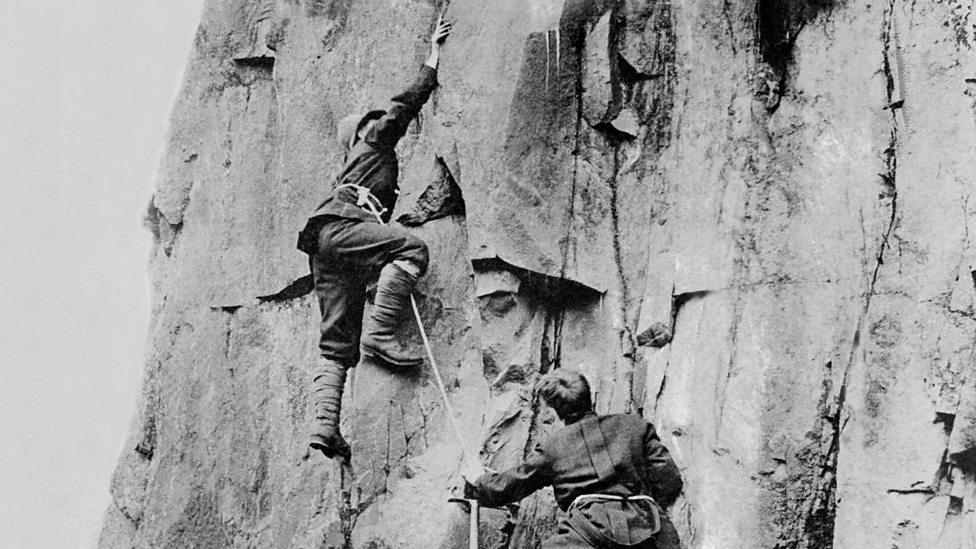
\includegraphics[width=0.75\linewidth]{figs/early-climbing.jpg}
    \caption{Early days of rock climbing}
\end{figure}

\section{Objectives}
The primary goal of this project is to conceptualize, design, and prototype a rotary climbing wall that revolutionizes endurance training for rock climbers. By providing a continuous rotating surface, this design simulates varying difficulties and overhang conditions, enhancing the indoor training experience for climbers.

\section{Motivation}
Indoor climbing facilities, particularly in South Africa, face spatial limitations that restrict the ability to train for endurance. Few climbing gyms offer high walls, limiting training opportunities for long-duration climbs. The development of a rotary climbing wall addresses this by providing an endless climbing surface, similar to a treadmill, enabling climbers to train on extended routes without the need for extensive vertical space.

\section{Problem Definition}
The primary challenge in rock climbing endurance training is the limitation of vertical space in indoor climbing gyms, particularly in regions like South Africa where facilities with high walls are scarce. Climbing endurance is a key component of performance, and current bouldering facilities, with walls of 4-5 meters, are insufficient for long-duration endurance training. \\\\
This project aims to solve this problem by developing a rotary climbing wall that offers a continuous climbing surface and simulates different difficulty levels and overhang conditions. The wall's rotating mechanism addresses the vertical space issue and provides climbers with the ability to train for endurance within a constrained space.

\section{Design Methodology}
The design methodology follows a systematic \textit{design, build, and test} approach, with the aim of addressing the problem outlined above. The methodology is divided into two main phases: conceptual design and detailed design.

\subsection{Phase I: Conceptual Design}
\begin{itemize}
    \item \textbf{Identification of Customer Needs:} Based on the problem definition, customer needs were identified to ensure the design aligns with the functional requirements of climbers who seek endurance training solutions.
    \item \textbf{Problem Definition:} The problem, as discussed in the previous section, focuses on the need for a continuous climbing surface to overcome vertical space limitations in traditional indoor climbing gyms.
    \item \textbf{Gathering Information:} A thorough review of technical articles, patents, and market solutions was conducted to inform the design. This is presented in Chapter \ref{chap:technology_review}.
    \item \textbf{Concept Generation:} Several design concepts were generated using creative brainstorming techniques. These concepts are detailed in Chapter \ref{chap:concept_design}.
    \item \textbf{Evaluation of Concepts:} The generated concepts were evaluated based on feasibility, cost, performance, and scalability.
    \item \textbf{Concept Integration:} The most suitable concept was selected and further refined into a comprehensive system design that addresses both functional and performance requirements.
    \item \textbf{Design Review:} A formal review of the final concept was conducted to ensure all requirements were met before transitioning to the detailed design phase.
\end{itemize}

\subsection{Phase II: Detailed Design}
\begin{itemize}
    \item \textbf{Design Verification:} The design was verified using structural and performance analysis, including Finite Element Method (FEM) simulations, to ensure it met safety and performance standards.
    \item \textbf{Detailed Engineering Drawings:} Engineering drawings were created to specify the dimensions, tolerances, and materials needed for manufacturing the rotary climbing wall.
\end{itemize}

\section{Use of Artificial Intelligence}
This report was composed in LaTeX, with AI assistance limited to spelling and grammar checks and enhancing the flow of certain paragraphs. Additionally, AI was used to support figure and table formatting in LaTeX but was not involved in the design, construction, or testing of the rotating climbing wall.


\chapter{Climbing Performance: Physiology and Training}
\label{chap:climbing_performance}

\section{Key Physiological Factors in Climbing}

Climbing is a complex sport that relies on of a combination of strength, power, endurance, and technique. The physiological attributes of strength, power, and endurance will be discussed here.

\subsection{Strength}
The concept of strength in climbing primarily focuses on the ability to exert a force consistently over a period of time, which is crucial for maintaining grip on climbing holds. This concept is further explained in an article by \citep{MaddyCope-2022} which mentions that when it comes to climbing, the upper body and finger flexors are two of the stand-out areas. \\\\
Key measures of climbing strength include the 2 Rep Max (2RM) pull-up and the 7-second maximum load hang tests, designed to assess a climber's static pulling power and grip strength. It is important to note that in this context, strength does not have a “race” or “explosive” element to it. The tests mentioned above focus on the capacity to sustain force without the necessity for velocity.\\\\
Effective strength training in climbing can be achieved by performing exercises that promote maximum strength with low repetitions \citep{Consuegra-2023}.

\subsection{Power}
The concept of power is slightly more complex, as it involves force and velocity. Specifically, power refers to the ability to exert force (or apply strength) explosively (at high rates). This results in forced applied being greatly increased for a short period of time.\\\\
Power is especially relevant when it comes to big, dynamic movements such as performing a dyno\footnote{A 'dyno' is when the climber makes a dynamic movement that uses momentum to get to the next hold. \citep{lafabriqueverticale_2022}} or similar movement.\\\\
Training power in climbing involves incorporating dynamic or explosive movements, such as campus board exercises, which are designed to improve both the speed and force of muscle contractions \citep{Consuegra-2023}.

\subsection{Endurance}
Endurance in climbing focuses on the climber's ability to sustain muscle activity over an extended period of time. A climber's endurance capability is essential when it comes to completing/sustaining performance on longer routes, as well as keeping performance levels from dropping throughout a climbing day. As outlined in \citep{Consuegra-2023}, endurance is categorized into power endurance, which involves high-intensity efforts over shorter timeframes, and muscular endurance, focusing on sustaining a sub-maximum effort over extended periods of time.\\\\
Endurance training involves interval climbing and repetitive route sessions, designed to enhance the climber's ability to improve metabolic efficiency at sub-maximum levels \citep{Consuegra-2023}.\\\\
\subsection{Training Guidelines and Methodologies}
The table below, as adapted from \citep{bechtel_endurance_2024}, presents various training methodologies categorized according to their focus on specific physiological aspects:
\begin{table}[H]
\centering
\caption{Climbing Training Categories}
\label{tab:climbing-training}
\begin{tabular}{@{}>{\raggedright\arraybackslash}p{2.5cm} 
                  >{\raggedright\arraybackslash}p{2cm} 
                  >{\raggedright\arraybackslash}p{1.5cm}>{\raggedright\arraybackslash}p{3cm} 
                  >{\raggedright\arraybackslash}p{4cm}@{}}
\toprule
\textbf{Training Goal} & \textbf{Duration} & \textbf{Number of Moves} & \textbf{Primary Focus} & \textbf{Primary Method of Training} \\ \midrule
Strength and Power    & 1-8 seconds      & 1-5                     & Single moves and boulder problems    & Hangboard, system wall, bouldering  \\
Power Endurance       & 9-120 seconds    & 6-30                    & Short routes and long boulders       & 2-3 problem links, traverse into problems, rhythm intervals \\
Muscular Endurance& 2 min to 10 min  & 30-150                  & Routes 40-90 feet in length          & 4-6 problem links, links on time interval, longer gym routes \\
\end{tabular}
\end{table}
\noindent
\\

\section{Climbing Disciplines and Associated Physiological Attributes}
According to \citep{brozek_climbing_2023}, there are three main disciplines involved in Competitive Sport Climbing, each requiring a unique set of skills to master. While competition holds significant relevance when it comes to training, the passion for outdoor climbing remains strong among many. To this end, Outdoor Lead Climbing and Bouldering have also been added here.\\\\
The flow diagram presented below delineates the primary physiological attributes associated with the main climbing disciplines. The diagram's line weights are adjusted to reflect the relative importance of each attribute, as informed by the data in Table \ref{tab:climbing-training}.

\begin{figure}[H]
    \centering
    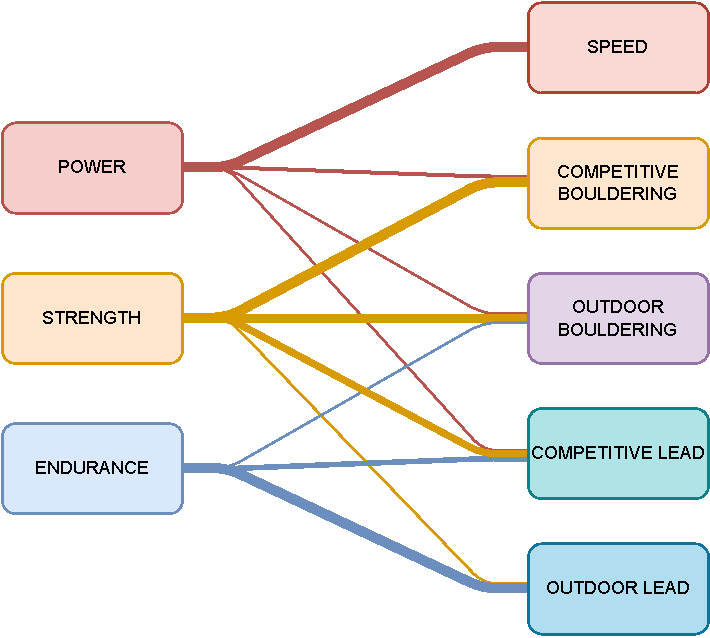
\includegraphics[width=0.9\linewidth]{figs/disciplines_physical.pdf}
    \caption{Physiological Attributes With Relation to Climbing Discipline Flow Diagram}
    \label{attribs-disc-flow}
\end{figure}
\noindent
The following breakdown of each discipline is adapted from \citep{bechtel_endurance_2024}

\subsection{Speed Climbing}
\begin{itemize}
    \item Goal: Climb to the top of the set route in the fastest possible time
    \item Wall: 15m with 5° overhang
    \item Time restriction: N/A. Current record as of 12 April 2024 is 4.79s, held by USA’s Sam Watson \citep{Fast2024}
    \item Skills in order of relevance: Power
\end{itemize}
In speed climbing, the main goal is to climb a standardized route on a  15m wall in the quickest possible time. In competition, two competitors race head to head with the first person to make it to the top, granted the victory. As the route is always the same, this aspect of the competition can be practised ahead of time. Safety is ensured by the participant wearing a harness attached to an automatic belay device. Because of the short duration of the event, power is the dominant attribute and endurance is not especially important.
\begin{figure}[H]
    \centering
    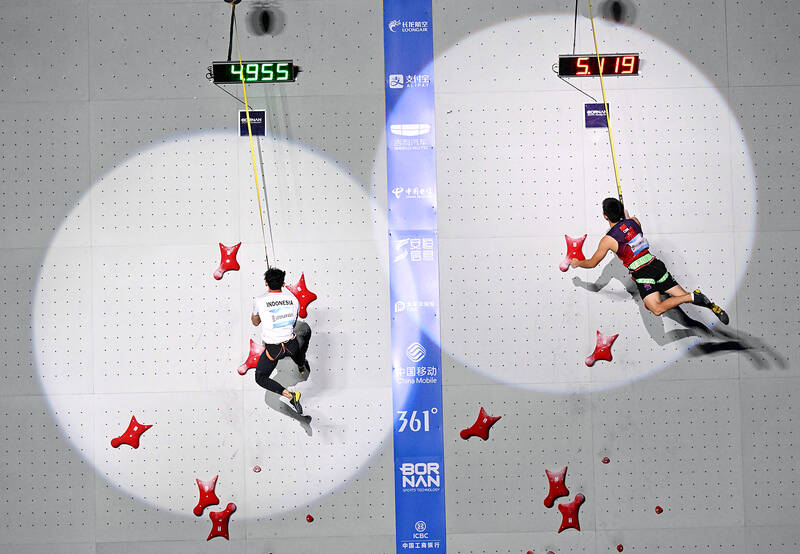
\includegraphics[width=0.9\linewidth]{figs/speed_climbing.jpg}
    \caption{Two speed climbers descend after reaching the top. \citep{Taipei_Times_2023}}
\end{figure}

\subsection{Competitive Bouldering}
\begin{itemize}
    \item Goal: To climb as many problems\footnote{In general, a boulder problem is a sequence of holds in a gym or outdoors that a climber has to navigate in order to reach the top.} as possible in the fewest possible moves
    \item Wall: 4m
    \item Time restriction: Four minutes for each problem
    \item Relevant Physiological Attributes: Strength, Power
    \end{itemize}
    Bouldering focuses on difficult problems of short duration / length. Participants climb without ropes, but mats or “bouldering pads” are placed beneath the climber for dismounting. Usually, boulder problems are overhanging and powerful, requiring a large amount of strength and power to complete.
    \begin{figure}
        \centering
        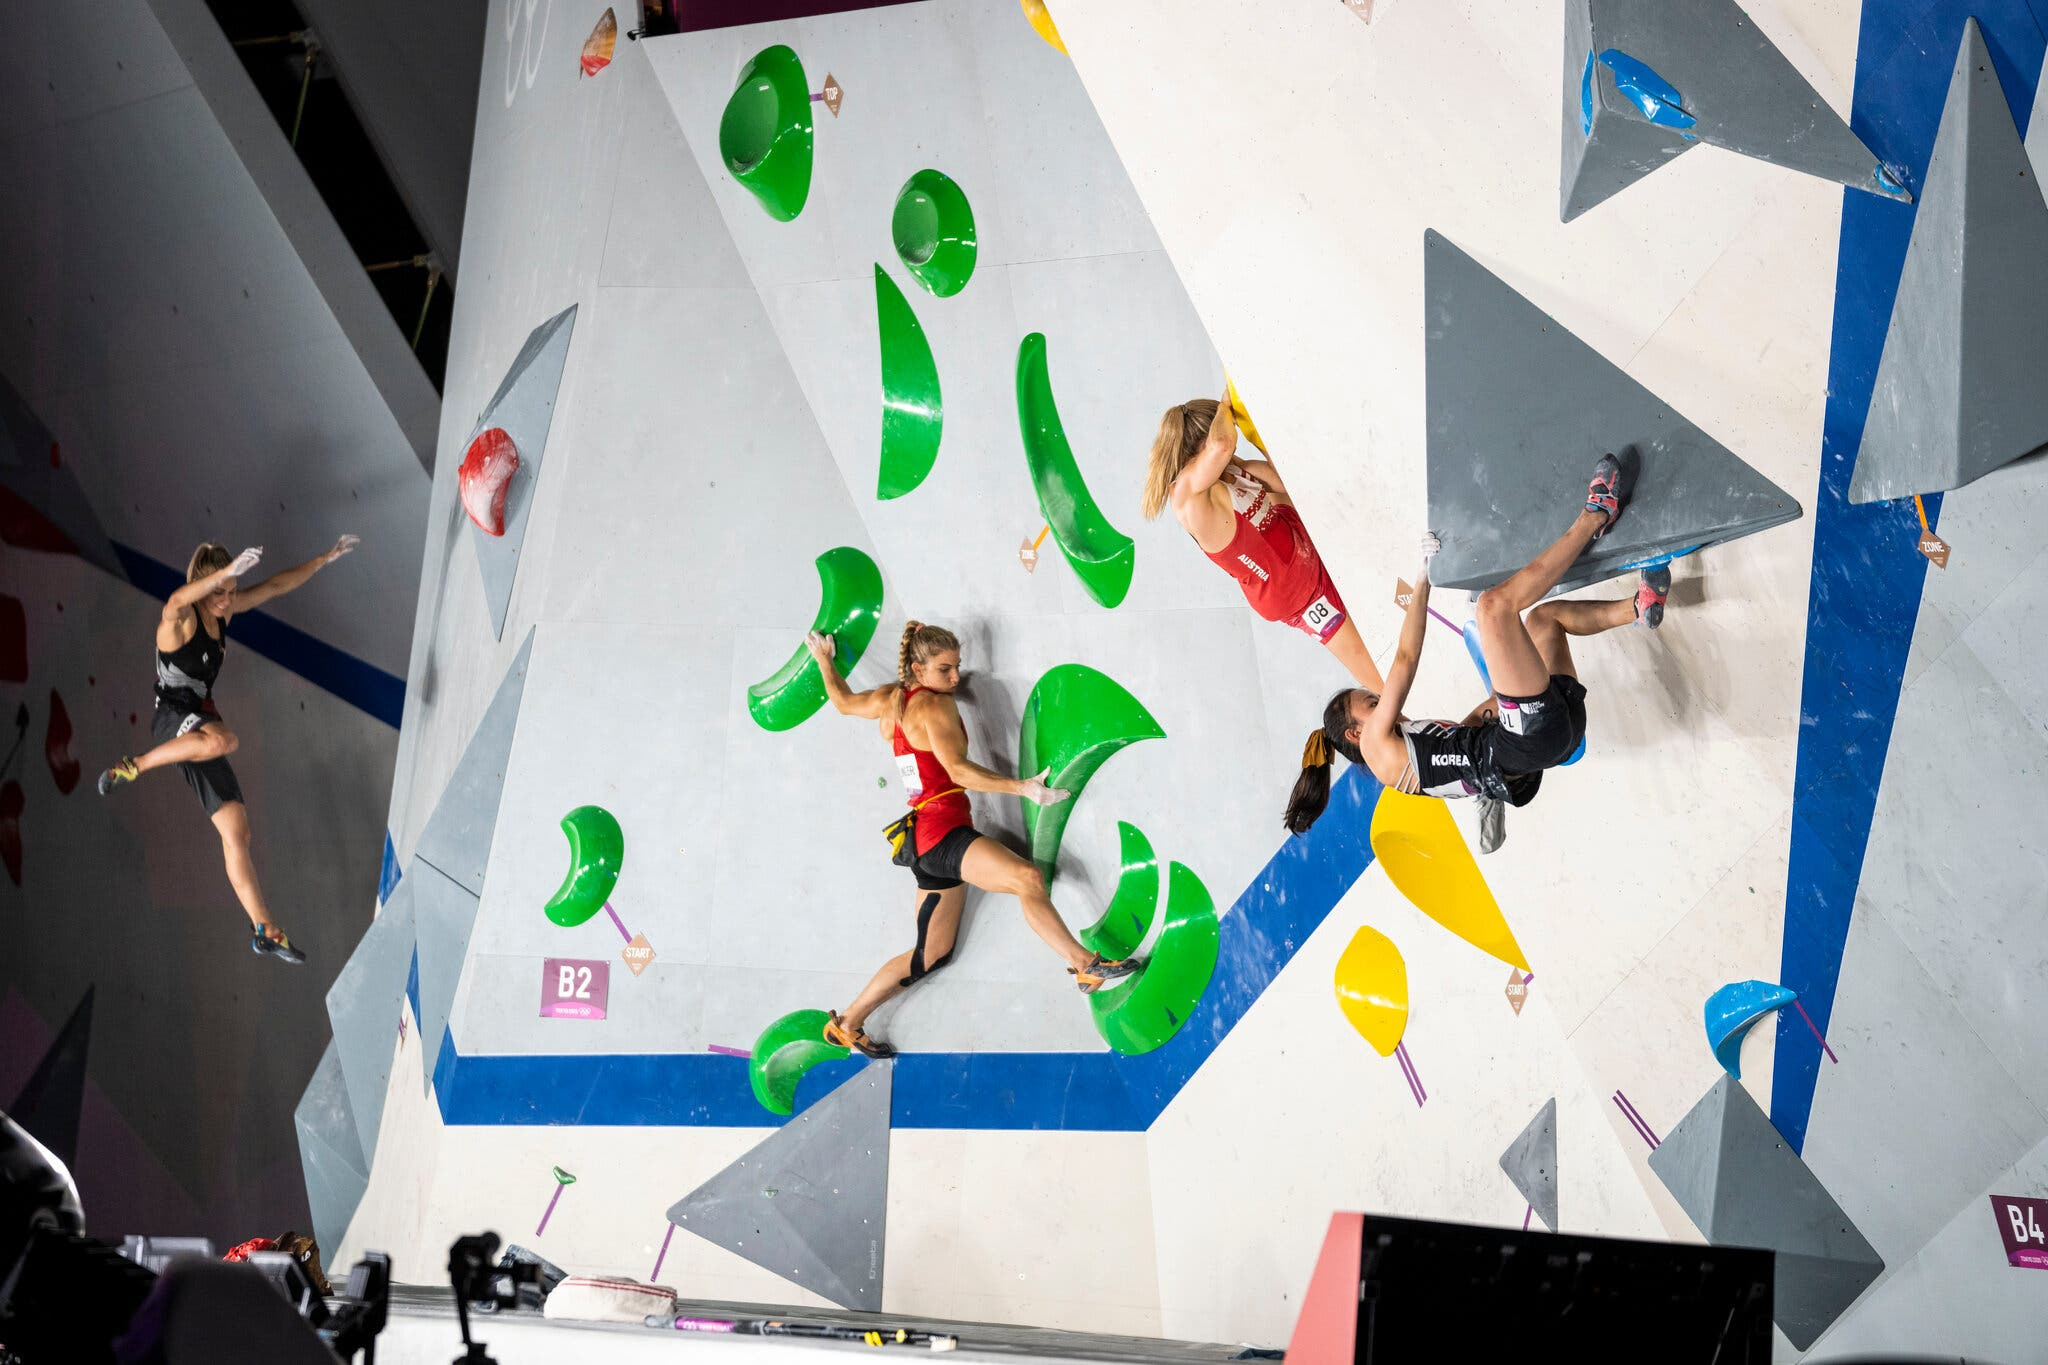
\includegraphics[width=0.9\linewidth]{figs/comp_bouldering.jpg}
        \caption{Bouldering at the 2020 Tokyo Olympics \citep{Branch_2021}}
    \end{figure}
\subsection{Outdoor Bouldering}
\begin{itemize}
    \item Goal: Similar to competitive bouldering but there is no time limit
    \item Wall: Varying height, incline
    \item Time restriction: N/A
    \item Relevant Physiological Attributes: Strength, Power, Endurance
    \end{itemize}
    Outdoor bouldering has no specified time limit. Climbers will attempt boulder problems of varying hight (generally below 4m), incline (usually overhanging) and difficulty for times varying from a few minutes (collectively) to many hours in a day. If many boulder problems are to be completed in a day, endurance will be of some importance.
    \begin{figure}[H]
        \centering
        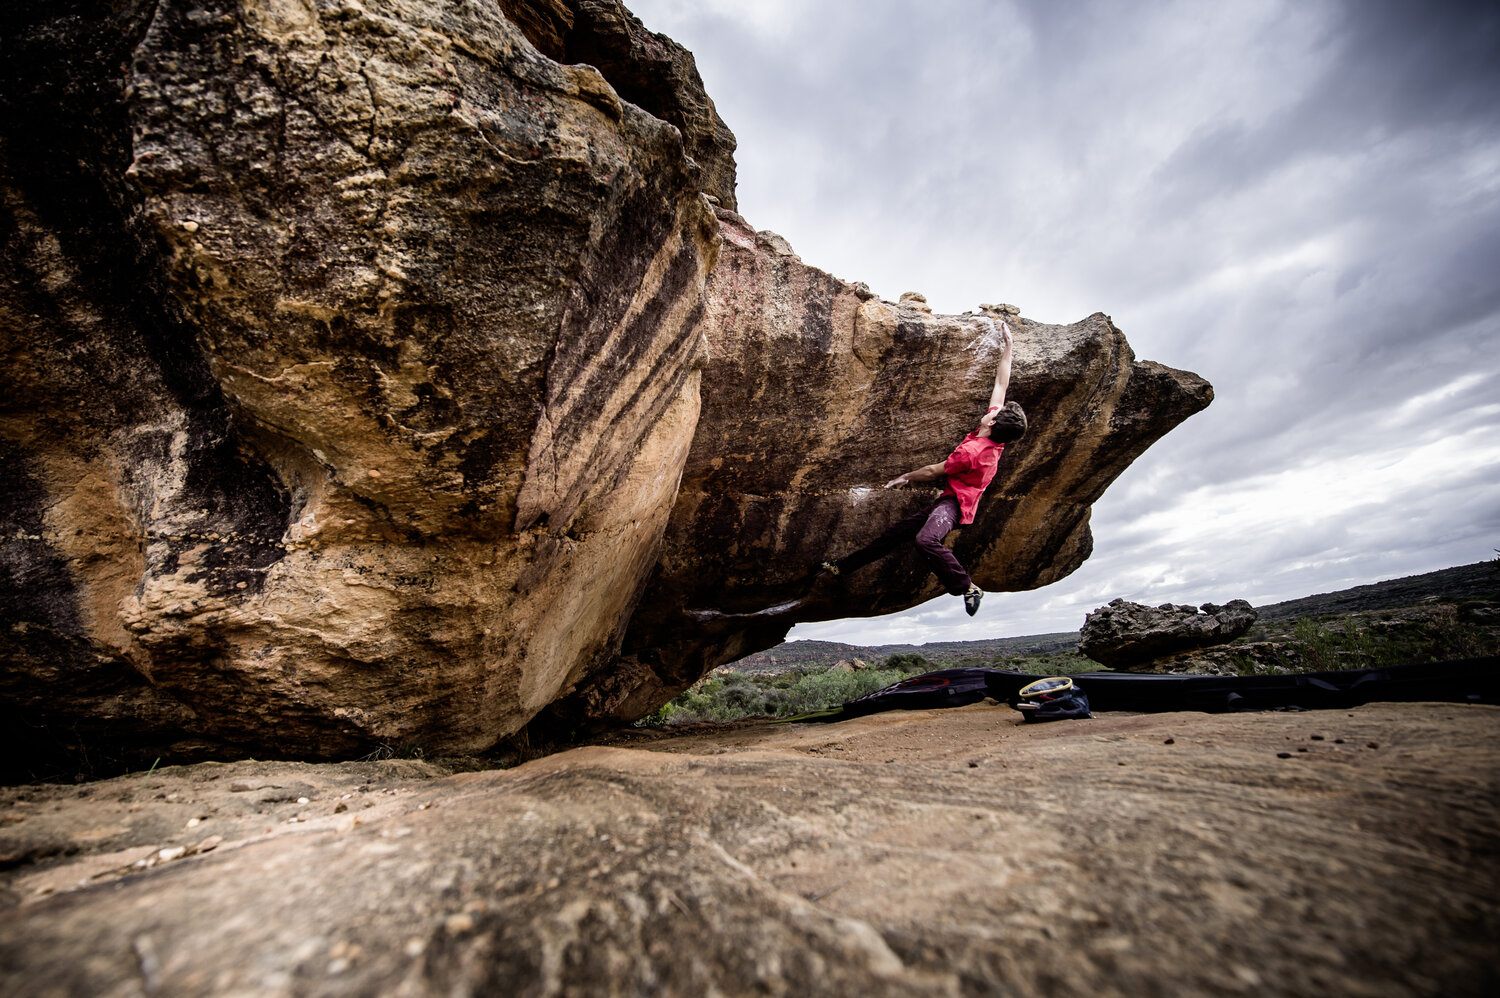
\includegraphics[width=0.9\linewidth]{figs/outdoor_bouldering.jpg}
        \caption{David Naude boudering outdoors, Rocklands, South Africa. \citep{Simon_2020}}
    \end{figure}

\subsection{Competitive Lead Climbing}
\begin{itemize}
    \item Goal: Climb as high as possible within time limit
    \item Wall: 15m with at least 7m overhang (overhang slope may vary on different sections of the route)
    \item Time restriction: Six minutes
    \item Skills in order of relevance: Endurance, Strength, Power
\end{itemize}
The aim when it comes to lead climbing, is for the athlete to climb as high as possible within six minutes. In the case that more than one competitor reaches the top, the person who got there the quickest is deemed the winner. Climbers make use of a rope which they must clip to anchor points along the route as they ascend. This clipping, combined with the increasing wall difficulty increases, and the fact that the walls are climbed without having been seen before by the climber, requires that the climbers pause at certain points to figure out their next move. Since the timeframe for this discipline is less than 6 minutes, the climber will mainly rely on strength endurance.
\begin{figure}[H]
    \centering
    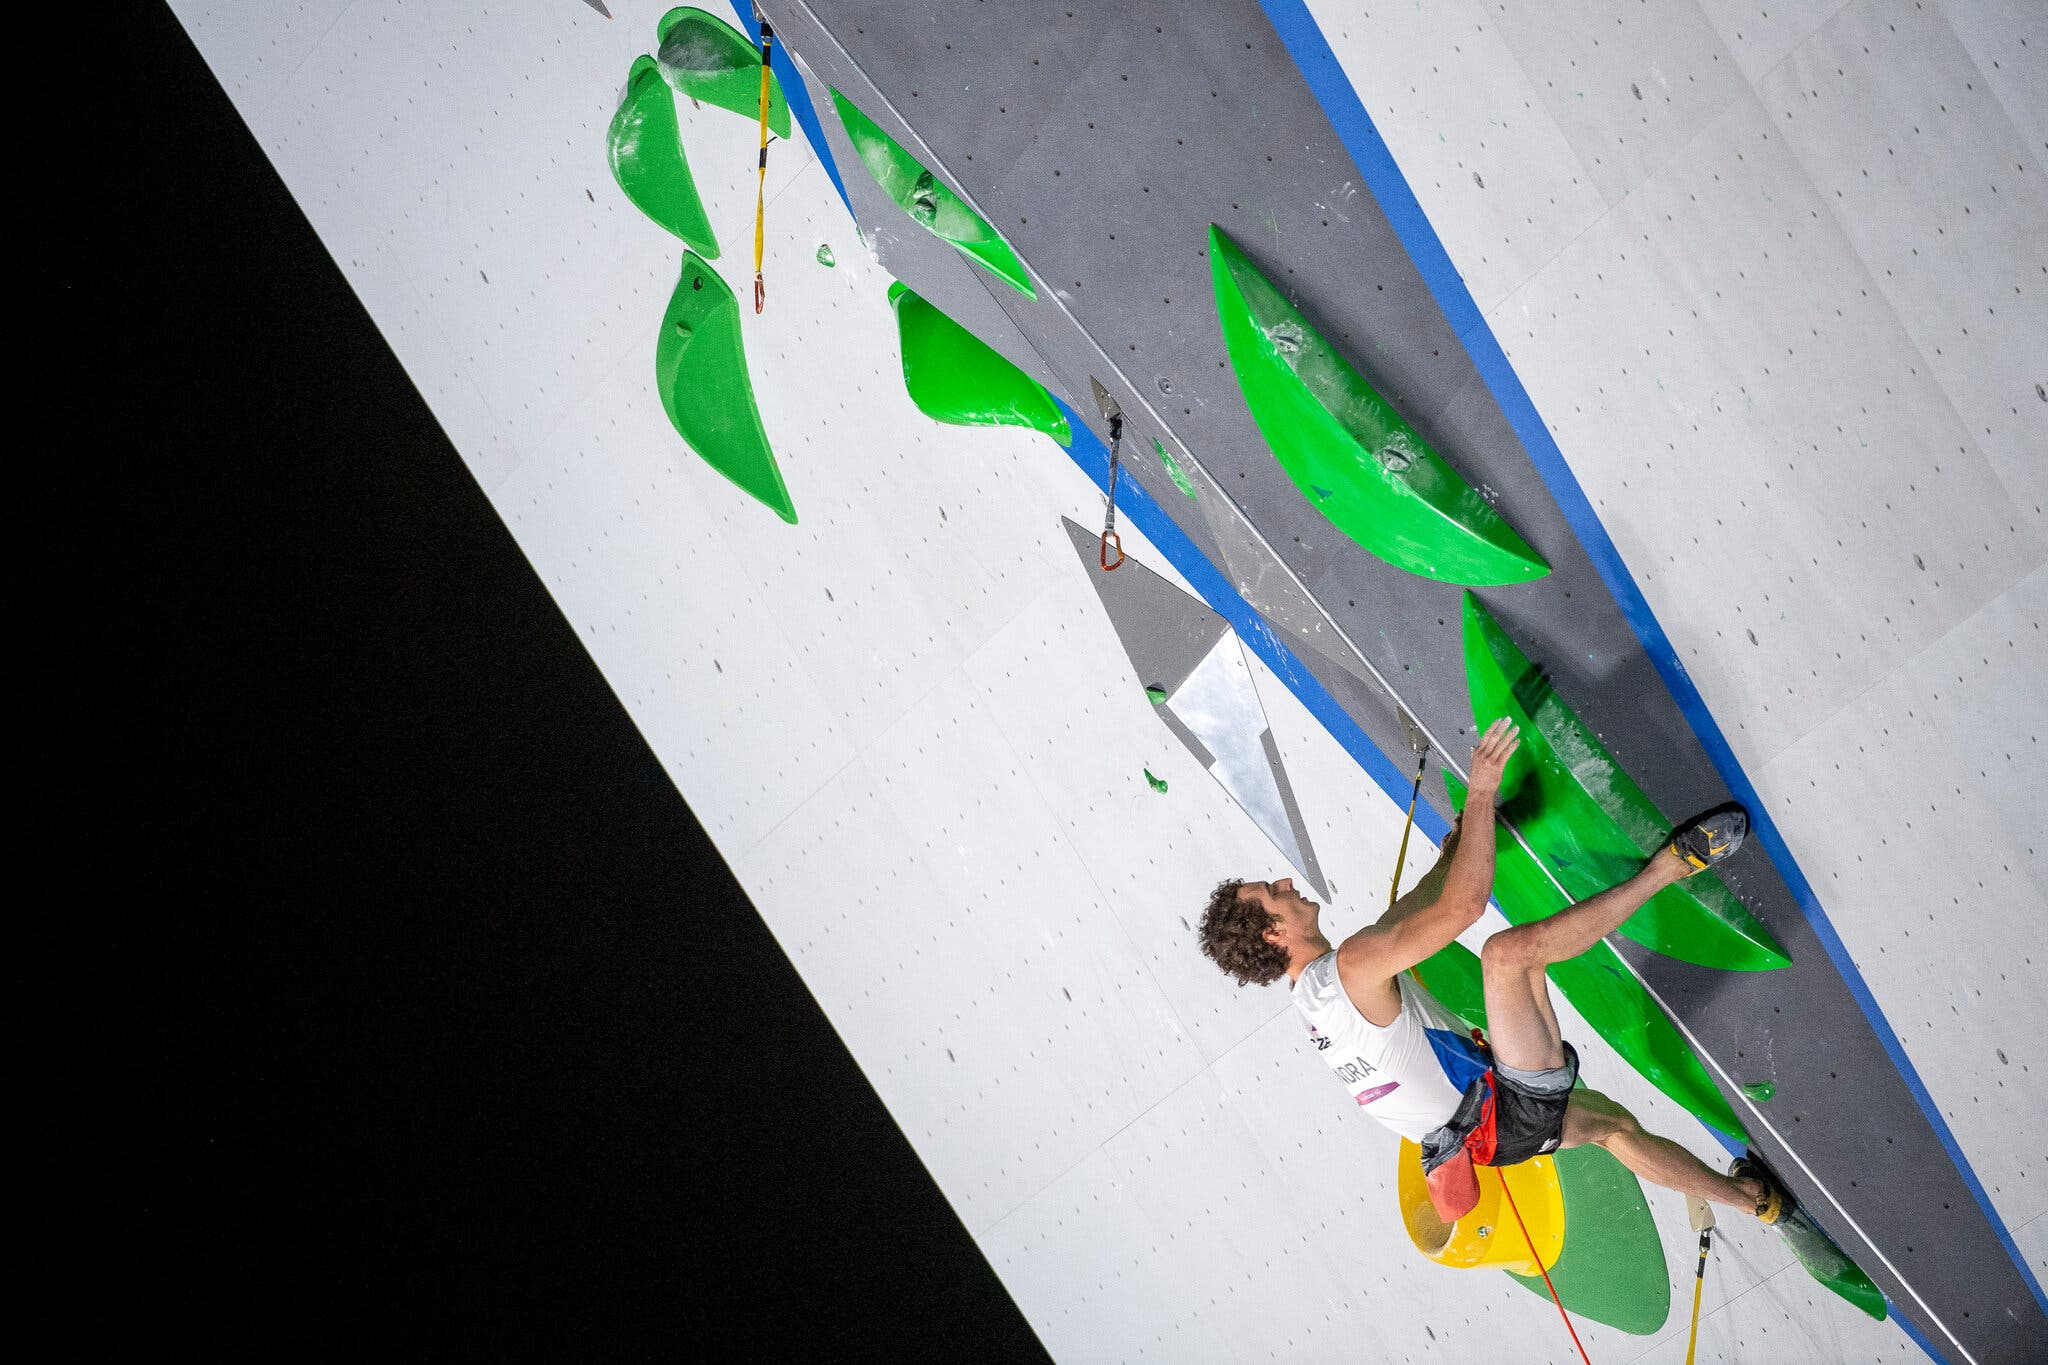
\includegraphics[width=0.9\linewidth]{figs/comp_lead.jpg}
    \caption{Adam Ondra competing in the lead portion of the 2020 Tokyo Olympics. \citep{Branch_2021}}
\end{figure}

\subsection{Outdoor Lead Climbing}
\begin{itemize}
    \item Goal: Similar to competitive lead, but there is no time limit.
    \item Wall: Varying height, incline
    \item Time restriction: N/A
    \item Skills in order of relevance: Endurance, Strength, Power
\end{itemize}
Outdoor lead climbing has no specified time limit. Climbers will attempt routes of varying height, incline, and difficulty for durations spanning from a few minutes to (collectively) several hours in a day of climbing. Here, muscular endurance is much more important.
\begin{figure}[H]
    \centering
    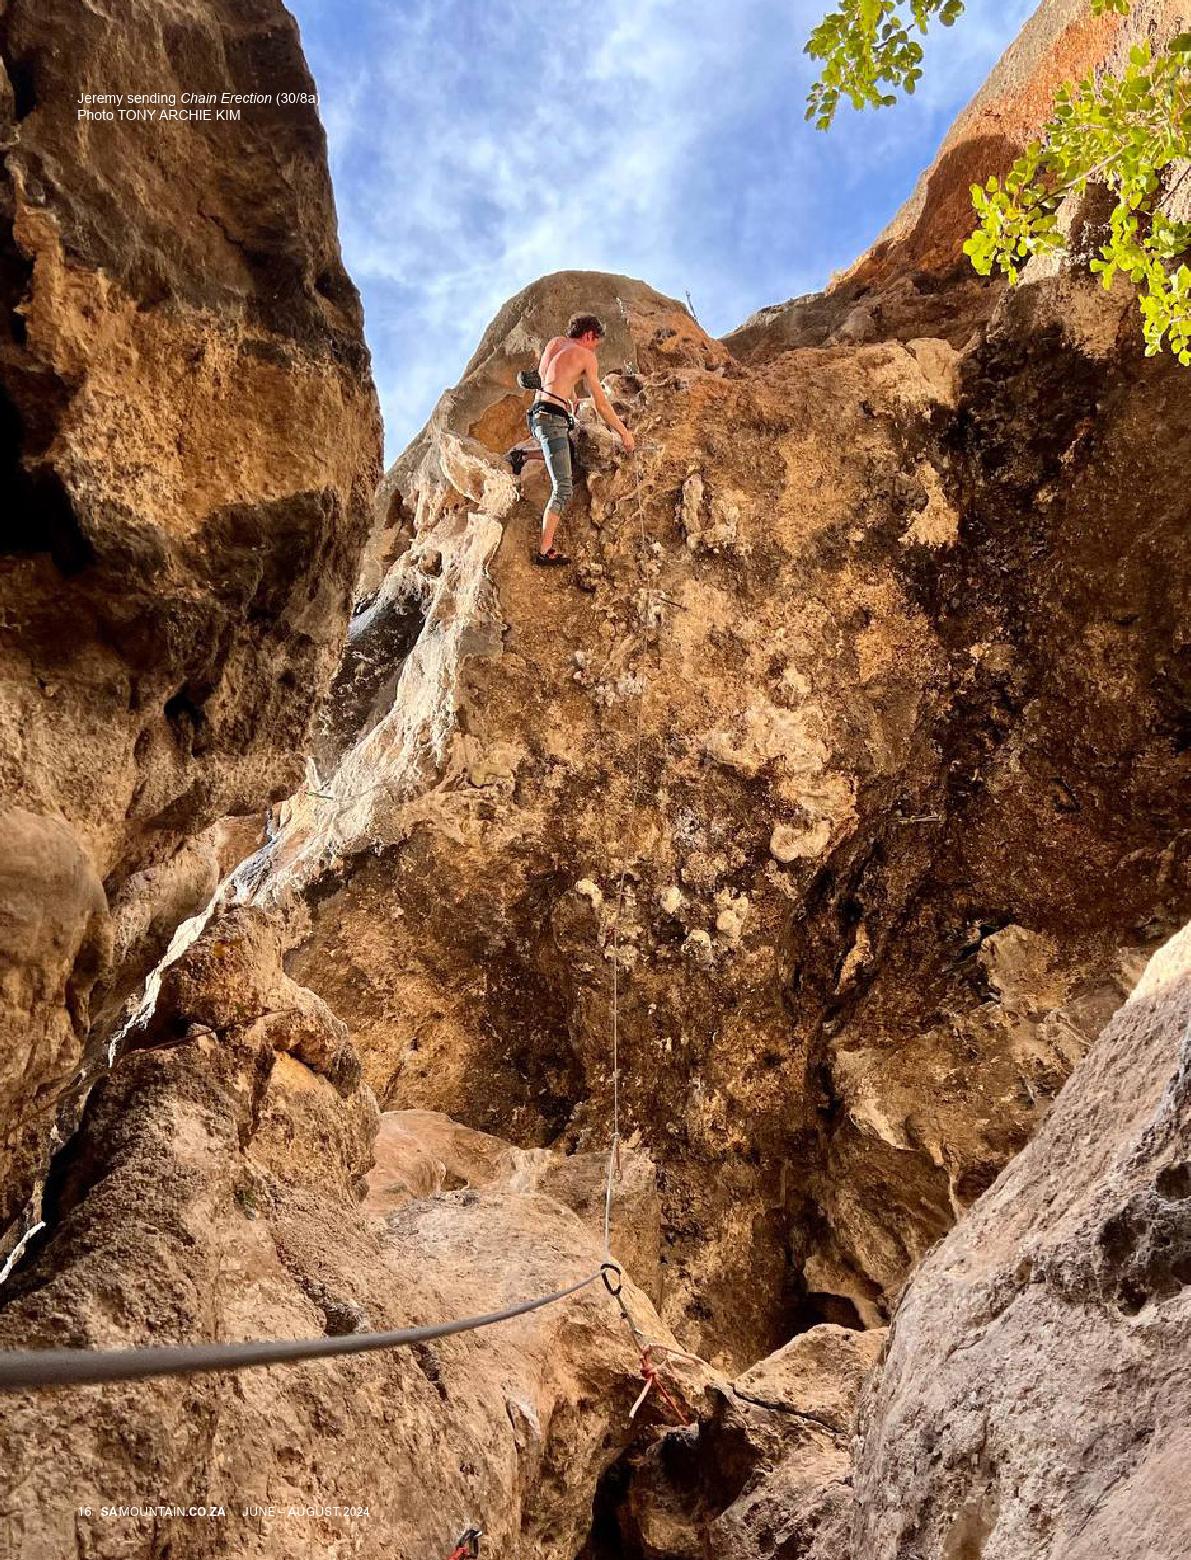
\includegraphics[width=0.9\linewidth]{figs/outdoor_lead.png}
    \caption{Jeremy van der Riet sending Chain Erection (30/8a). Photo by Tony Archie Kim. Source: SA Mountain Magazine, June-August 2024}
\end{figure}




\chapter{Technology Review}
\label{chap:technology_review}

\section{Overview of Patented Climbing Wall Technologies}

The US Patent US5919117A entitled: 'Climbing Training Apparatus' \cite{US5919117A} describes the device as being “a movable climbing training wall surface defined by a continuous belt rotatably disposed about a pivotable frame and controllably actuated to rotate at a selected speed”.\\
The patent was filed on 1999-07-06 and subsequently expired on 2017-01-29. It is now classified as Expired - Fee Related.\\\\
A similar patent US005125877A entitled: 'Simulated Climbing Wall' \cite{US5125877A} also describes a rotating climbing device. This patent is also expired.\\\\
There is thus currently no commercial restriction on rotating climbing apparatus and simulated climbing walls and this project is therefore able to proceed with development of a rotary climbing wall.

\section{Analysis of Current Climbing Wall Models}
The rotating climbing wall market currently offers a range of products, from higher-end systems equipped with extensive features as well as more economic systems with fewer functionality. \\\\
After evaluating the current systems available, the list below outlines the main functions currently available on the market:

\begin{itemize}
    \item Adjustable Speed
    \item Adjustable Incline
    \item Automatic pause/continue rotation
    \item Can operate without electricity
    \item Monitor Results
    \item Automatic Climbing modes/difficulty
\end{itemize}

\subsection{Xclimbpro Rotating Climbing Wall} (\url{https://xclimbpro.com/})
\begin{figure}[H]
    \centering
    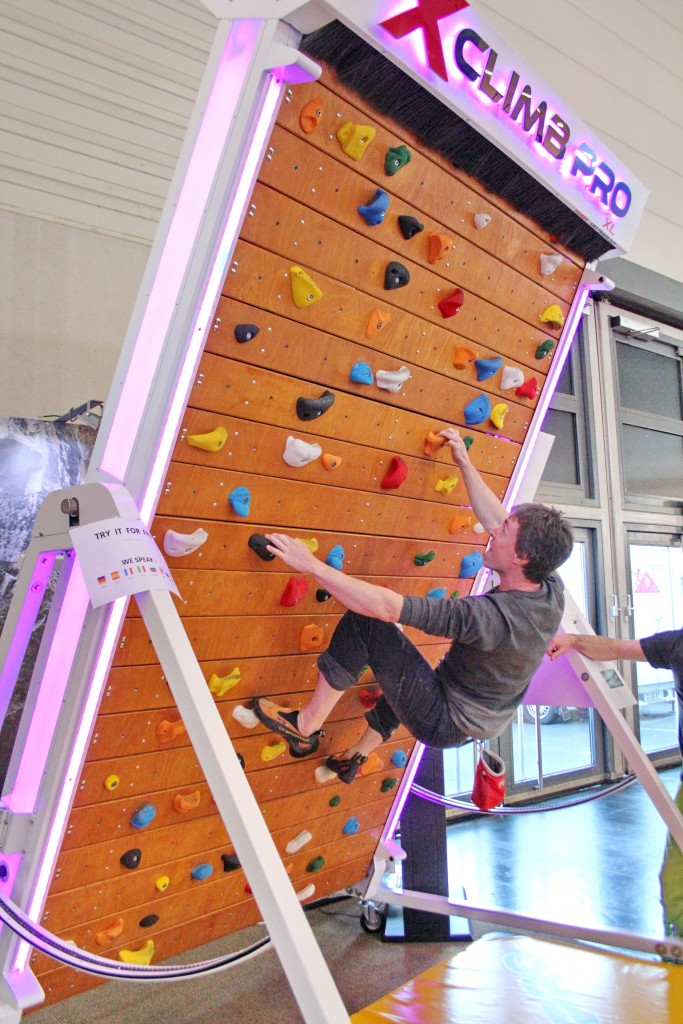
\includegraphics[width=0.6\linewidth]{figs/Xclimbpro.jpg}
    \caption{Xclimbpro Rotating Climbing Wall}
\end{figure}
    \begin{itemize}
        \item Features adjustable speed and can operate without electricity, offering an optional 12V adapter.
        \item Offers versatility in installation, being wall-mountable or movable with optional casters.
        \item Models include:
        \begin{itemize}
            \item Model S: Compact and budget-friendly.
            \item Model M: Features increased width and angle adjustment from +35° to -35°.
            \item Model L: Offers larger dimensions for all skill levels.
            \item Model XL: Stands 3.5m tall, accommodating 2-3m climbers with a -35° inclination.
        \end{itemize}
    \end{itemize}

\subsection{Climbstation Climbing Wall}
(\url{https://www.climbstation.com/})
\begin{figure}[H]
    \centering
    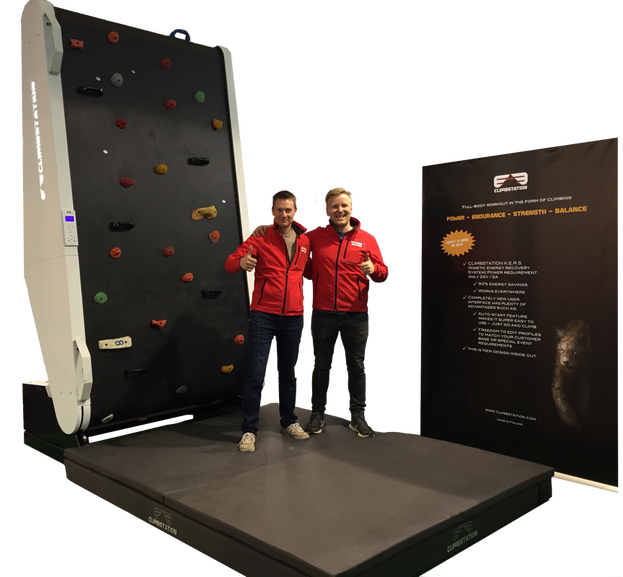
\includegraphics[width=0.9\linewidth]{figs/climbstation.png}
    \caption{Climbstation Climbing Wall}
\end{figure}
    \begin{itemize}
        \item The operational size is 330 cm in height by 190 cm in width and 380 cm in length.
        \item Allows for adjustable climbing surface angles from +15° to -45°.
        \item Achieves the highest climbing speed of 25 meters per minute.
        \item Includes 70 standard handholds, 
        \item Powered by a 24-30V / 2A / 50-60Hz source.
        \item Key functions and features include Terrain Editor, Restore Function, Climb Data and Payment System Support, Unlimited Climbing Options, and Monitoring of Results.
    \end{itemize}

\subsection{TreadWall}
(\url{https://treadwallfitness.com/})
\begin{figure}[H]
    \centering
    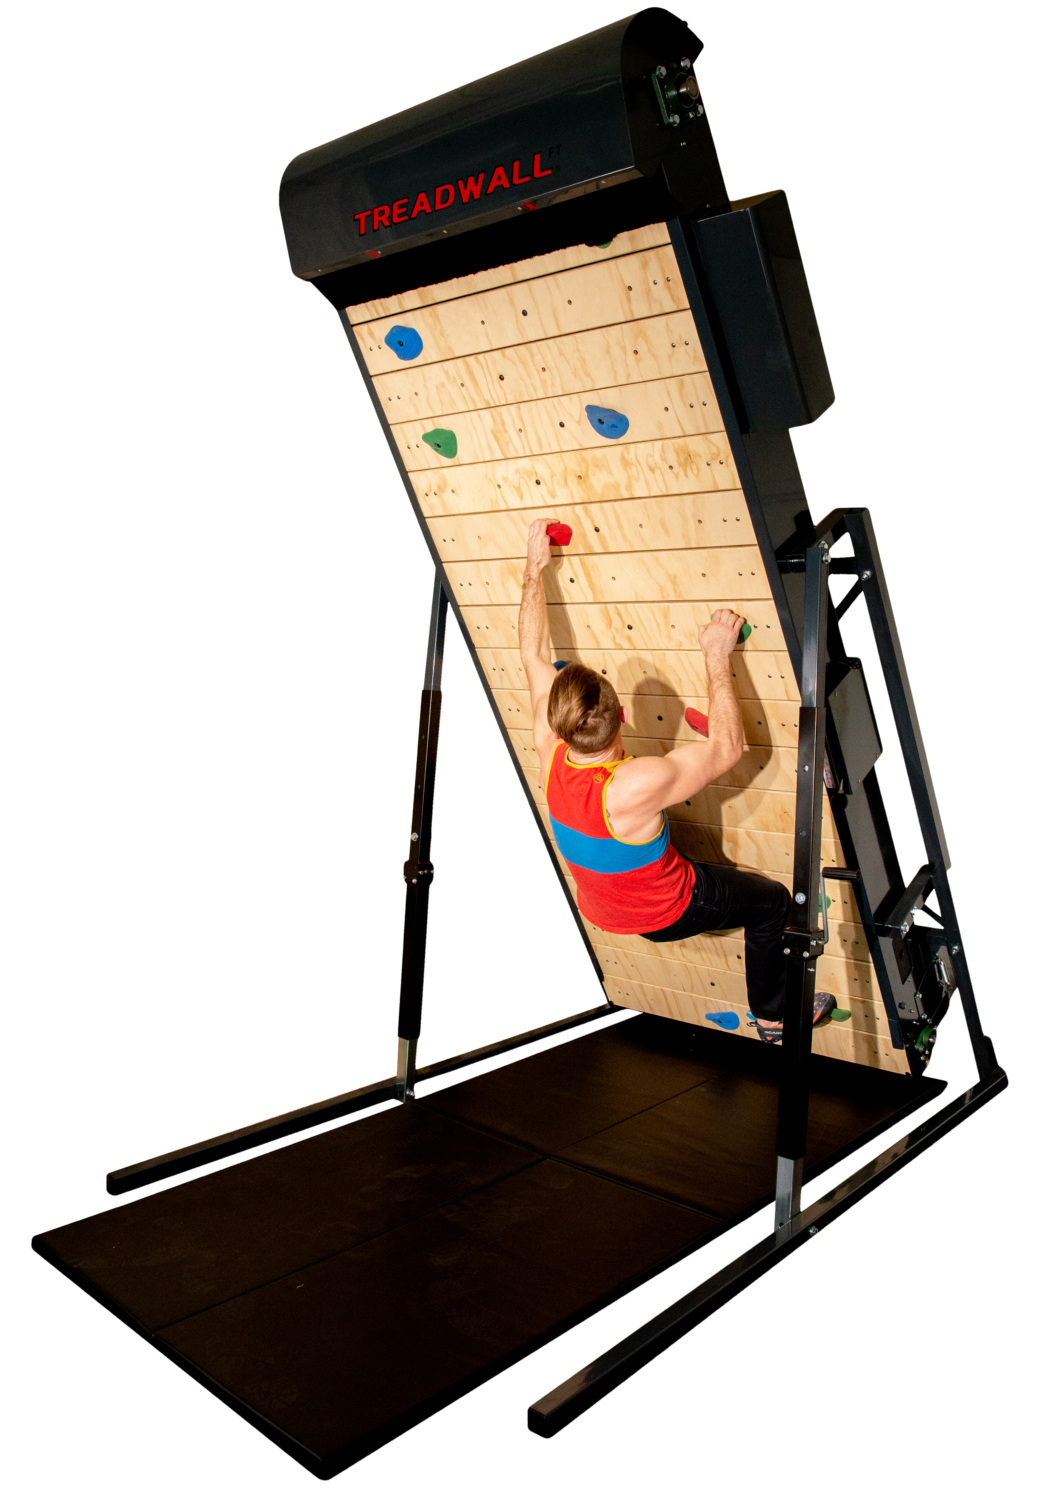
\includegraphics[width=0.5\linewidth]{figs/treadwall_kore4.png}
    \caption{Treadwall Kore4}
\end{figure}
    \begin{itemize}
        \item Features adjustable speed and some models can operate without electricity.
        \item Features adjustable inclination, with certain models adjusting this automatically and others manually.
        \item Automatically pauses when climber's weight on bottom rung.
        \item 180 possible hold placements
        \item Features electronic display that measures speed, distance,  time, and calories.
        \item Models include:
        \begin{itemize}
            \item V4: Base model without incline ability.
            \item Kore4: Budget model for home use. Features incline ability.
            \item S4: Larger model for gym use. All features available.
            \item Max6: Flagship model with a 3.1m height and 1.83m width. All features available
        \end{itemize}
        
    \end{itemize}

\section{Detailed Product Comparisons}
The table below provides a comprehensive summary of the functionalities available in each product.

\begin{table}[H]
\centering
\caption{Comparison of Climbing Wall Models}
\label{tab:climbing_wall_comparison}
\resizebox{\textwidth}{!}{%
\begin{tabular}{|p{0.12\linewidth}|p{0.08\linewidth}|p{0.08\linewidth}|p{0.1\linewidth}|p{0.1\linewidth}|p{0.1\linewidth}|p{0.12\linewidth}|p{0.2\linewidth}|p{0.1\linewidth}|}
\hline
System & Width [m] & Height [m] & Incline & Adjust\newline Speed & Monitor & Extra\newline Functions & Construction\newline Material & Price \\
\hline
XClimb\newline Pro S & 1.5 & 2.82 & No & Yes & No & No & Steel/Wood & R230000 \\
\hline
XClimb\newline Pro XL & 2 & 3.48 & Auto& Yes & No & No & Steel/Wood & R278000 \\
\hline
Climb\newline Station & 1.9 & 3.3 & Auto& Auto & Yes & Advanced Control\newline Panel & Aluminium & N/A \\
\hline
Treadwall V4 & 1.22 & 2.97 & No & Manual & Yes & auto-stop & Steel/Wood & R202000 \\
\hline
Treadwall Kore4/11 & 1.22 & 2.75 & Manual & Manual & Yes & auto-stop & Steel/Wood & R140600 \\
\hline
Treadwall S4/12 & 1.22 & 3.1 & Manual & Manual & Yes & auto-stop & Steel/Wood & R218000 \\
\hline
Treadwall Max6/12 & 1.83 & 3.1 & Manual & Manual & Yes & auto-stop & Steel/Wood & R227200 \\
\hline
\end{tabular}
}
\end{table}

\section{Selection of Features for Proposed Climbing Wall Design}
In order to effectively train the three core physiological pillars of climbing—strength, power, and endurance—the design of the rotary training device must feature adjustable speed and inclination. While additional functionalities such as automatic adjustments for speed and inclination during use, along with metrics for tracking distance climbed and calories burned, may enhance usability, they are not essential for this prototype.\\\\
From the analysis presented in Table \ref{tab:climbing_wall_comparison}, as well as general design overview, a few unique concepts for each sub-system were derived.




\chapter{Concept Design}
\label{chap:concept_design}

\section{Introduction}

This chapter presents a detailed outline of the design process for a rotating climbing surface, emphasizing the mechanical design principles integrated with electronic and computer system engineering. The project's primary aim is to design and manufacture a rotating climbing surface capable of providing a facility for extended-duration indoor climbing.

\section{Problem Definition}
\label{sec:problem_definition}

This project aims to develop a rotating climbing surface capable of rotating at a constant, user-defined speed and adjustable incline. The system must exhibit precise control over both speed and incline, as well as incorporate safety measures for user safety.

Key aspects of the project include the design and implementation of robust mechanical and electronic systems to facilitate smooth operation, integrating sensor technologies for accurate speed and inclination detection, and developing an intuitive and simplistic user interface for seamless interaction.

The rotating climbing surface should also adhere to stringent safety guidelines to mitigate potential hazards associated with operation. This encompasses utilizing calculations and simulations to ensure structural integrity, as well as a series of load tests that will need to be passed.

\section{Stakeholder Requirements}

The stakeholder requirements define the intended services of the system and the restrictions on achieving them.

\begin{table}[H]
\centering
\caption{Stakeholder Requirements}
\label{tab:stakeholder-requirements}
\begin{tabular}{|>{\centering\arraybackslash}p{0.12\linewidth}|>{\raggedright\arraybackslash}p{0.17\linewidth}|>{\raggedright\arraybackslash}p{0.5\linewidth}|>{\centering\arraybackslash}p{0.11\linewidth}|}
\hline
\textbf{Number}  & \textbf{Stakeholder} & \textbf{Description} & \textbf{Priority} \\
\hline
SR1  & End-user & Simulate continuous climbing & Must Have \\
SR2  & End-user & Incline adjustment for different difficulty levels & High \\
SR3  & End-user & User-adjustable speed control to accommodate various training intensities & Must Have \\
SR4  & End-user, Safety Officer & Durable and safe construction to withstand continuous use & High \\
SR5  & End-user, Safety Officer & Emergency stop feature for immediate halting of the wall for user safety & Must Have \\
SR6  & End-user & Large enough surface for comfortable climbing experience & High \\
SR7 & Investor, Customer & Affordability & Medium \\
\hline
\end{tabular}
\end{table}

\section{Engineering Requirements}

The stakeholder requirements given in the previous section were expressed by the design team as functional requirements (FRs) in Table \ref{tab:functional-requirements} and performance requirements (PRs) in Table \ref{tab:performance-requirements}. Where relevant, the number of the stakeholder requirement that the engineering requirement was derived from is indicated in the right-hand column. FRs give the actions that the system being designed must do, as seen by the stakeholders. Internal or derived functions are considered in later sections. The PRs are measures of how well the system should perform its functions.

\begin{table}[H]
\centering
\caption{Functional Requirements}
\label{tab:functional-requirements}
\begin{tabular}{|c|p{0.6\linewidth}|>{\centering\arraybackslash}p{0.2\linewidth}|}
\hline
\textbf{FR Number} & \textbf{Description} & \textbf{Related Stakeholder Requirement} \\
\hline
FR1 & Speed control and adjustment & SR1, SR3 \\
FR2 & Incline control and adjustment & SR2 \\
FR3 & Simplistic user interface & SR3, SR5 \\
FR4 & Safety mechanisms & SR5 \\
FR5 & Size compliance & SR6 \\
FR6 & Load compliance & SR6 \\
\hline
\end{tabular}
\end{table}

\begin{table}[H]
\centering
\caption{Performance Requirements}
\label{tab:performance-requirements}
\begin{tabular}{|c|p{0.4\linewidth}|c|c|c|c|}
\hline
\textbf{PR} & \textbf{Description} & \textbf{Target} & \textbf{Range} & \textbf{Unit} & \textbf{Related FR} \\
\hline
PR1 & Maximum rotation speed & 25 & 0--25 & m/min & FR1 \\
PR2 & Maximum negative inclination angle & -45 & -30 to -45 & degrees & FR2 \\
PR3 & Maximum positive inclination angle & +15 & +10 to +20 & degrees & FR2 \\
PR4 & Emergency stop halt time & $<$1 & $<$2 & seconds & FR4 \\
PR5 & Load capacity of climbing wall & 100 & 0--100 & kg & FR6 \\
PR6 & Climbing surface width & 1.5 & 1.4--1.6 & m & FR5 \\
PR7 & Climbing surface height & 2.9 & 2.5--3.1 & m & FR5 \\
\hline
\end{tabular}
\end{table}

\section{Subsystem Identification and Selection}
\label{sec:concept_selection}

Based on the specified requirements and specifications of the rotating climbing surface, several key subsystems are crucial for the design and implementation of the system.

\subsection{Subsystem Identification}

\begin{enumerate}
    \item \textbf{Inclination Adjustment System:} Allows the inclination of the rotating climbing surface to be adjusted to vary difficulty levels.
    \item \textbf{Braking System:} Responsible for controlling the rate of rotation, thus controlling the speed of the climbing surface. The speed should be constant and smooth.
    \item \textbf{Rotating Surface:} The physical surface that rotates, allowing climbing holds to be mounted on it.
    \item \textbf{Control System and User Interface:} Serves as the connection between the user's preferences and the control of inclination and speed. It must be intuitive and user-friendly, enabling clear adjustment control over the necessary parameters.
    \item \textbf{Safety System:} Able to cut power to all high-power electronics and allow rotation to come to a rapid stop as soon as the emergency stop button is activated. The system should also ensure that all electronics and moving parts are enclosed.
\end{enumerate}

\subsection{Functional Decomposition}

The functional requirements detailed previously outline the actions the rotating climbing wall system must perform from the stakeholders' perspective. In this section, these requirements are further decomposed to identify the internal functions the system must execute. Figure~\ref{fig:functional-decomp} illustrates the flow of energy, information, and materials to and from the functions that consume, generate, or transform these flows within the rotating climbing wall system.

\begin{figure}[H]
    \centering
    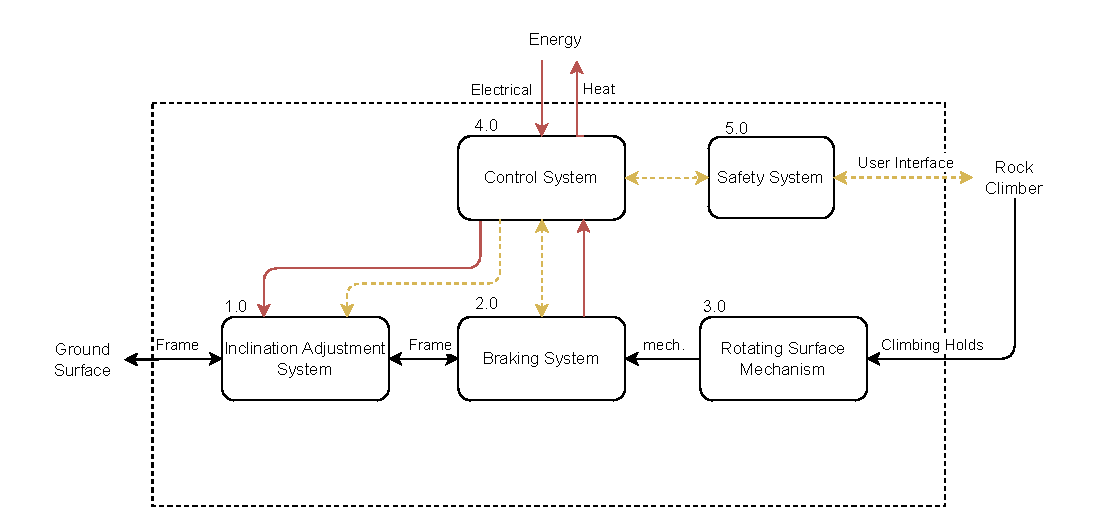
\includegraphics[width=1\linewidth]{figs/concept_design/Functional_Decomp_Flow.pdf}
    \caption{Top-Level Functional Decomposition}
    \label{fig:functional-decomp}
\end{figure}

\section{Concept Development}

\subsection{Inclination Adjustment System}

The inclination adjustment system allows for altering the climbing angle of the wall, making it more beginner-friendly with less steep angles or more challenging with overhangs for advanced climbers and intense training sessions. This subsystem addresses FR2 (Incline control and adjustment) and PR2 and PR3 from the performance requirements.

\subsubsection{Concept Generation}

\paragraph{IAS1: Linear Actuation}

This concept uses linear actuators connected to the frame of the climbing wall to adjust its angle. The actuators can be controlled electronically, allowing for precise and automated inclination adjustments through a user interface. Basic calculations (see Appendix~\ref{calcs:linear-actuator}) were performed which indicate that very high-force actuators would be needed for this sub-system, making it an expensive choice.

\begin{figure}[H]
    \centering
    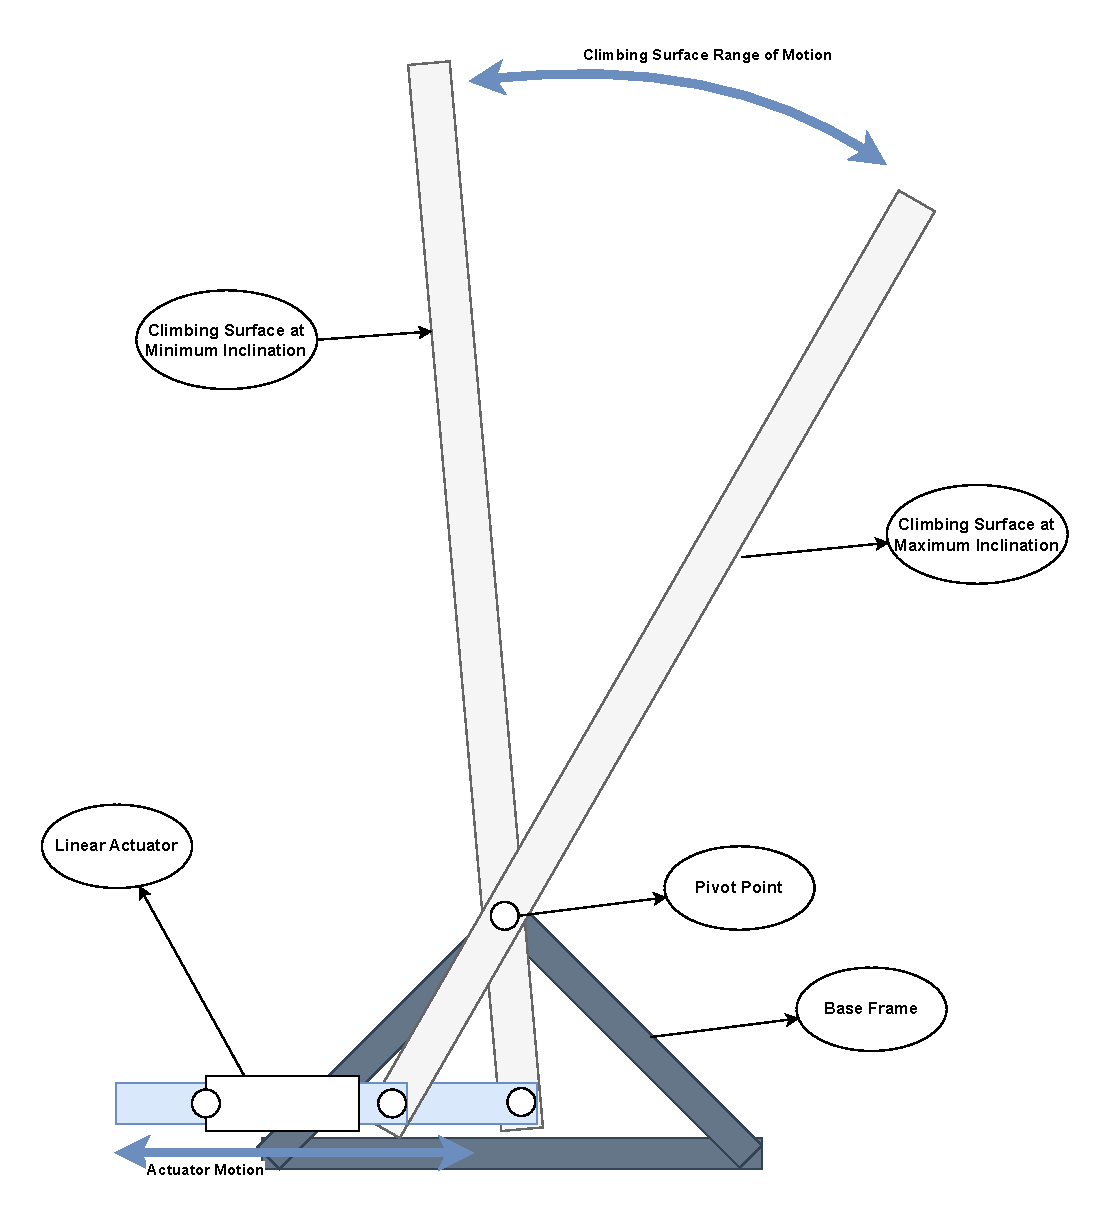
\includegraphics[width=0.6\linewidth]{figs/concept_design/Linear_Actuator_Concept.pdf}
    \caption{Linear Actuator Concept Sketch}
    \label{fig:linear-actuator-concept}
\end{figure}

\textbf{Advantages:}
\begin{itemize}
    \item Precise and automated control over inclination.
    \item Fairly safe method of inclination.
    \item Fairly simple design.
\end{itemize}

\textbf{Disadvantages:}
\begin{itemize}
    \item Higher cost due to actuators.
    \item Decreased range of motion due to actuator movement limitations.
\end{itemize}

\paragraph{IAS2: Hand-Crank Inclination}
This manual method incorporates a large curved rack fastened to the base frame and a hand-crank powered pinion driving the angle adjustment of the rest of the system.

\begin{figure}[H]
    \centering
    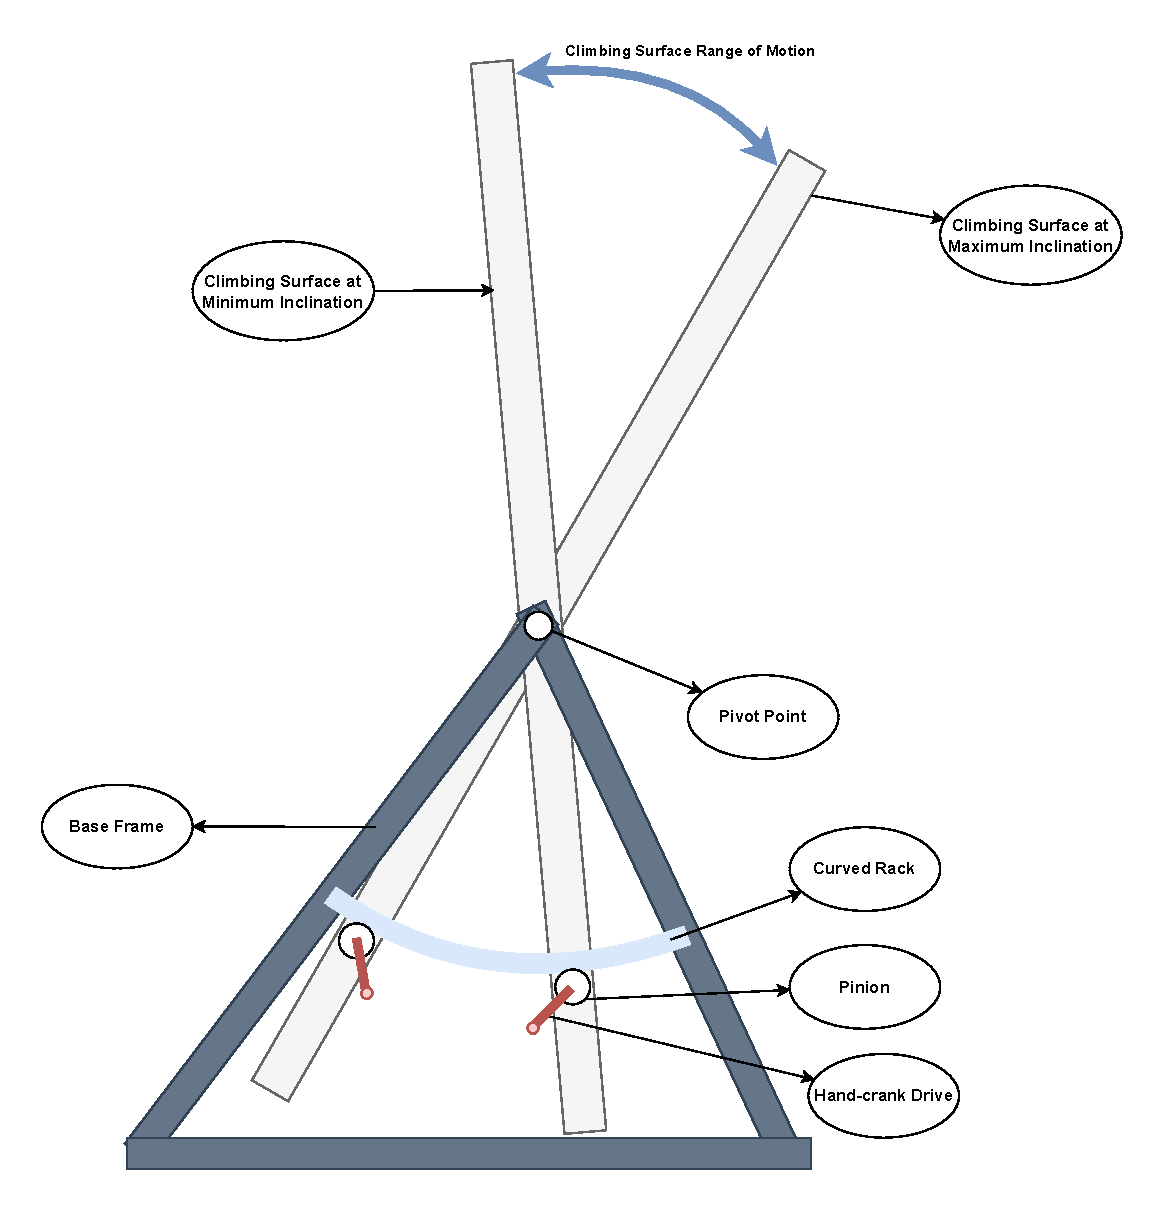
\includegraphics[width=0.6\linewidth]{figs/concept_design/Handcrank_Concept.pdf}
    \caption{Hand-Crank Inclination Concept Sketch}
    \label{fig:handcrank-concept}
\end{figure}

\textbf{Advantages:}
\begin{itemize}
    \item Low cost and simplicity.
\end{itemize}

\textbf{Disadvantages:}
\begin{itemize}
    \item Requires manual effort, which may be inconvenient.
    \item Lacks precision and repeatability of training inclination angle.
    \item Safety concerns due to operator being very near the machine. Potential for spinning handle if operator loses control.
    \item Extra mechanism/pin required to lock angle in place.
\end{itemize}

\paragraph{IAS3: Worm Gear Automatic Inclination}

This concept is very similar to the manual adjustment concept with the addition of a motor-driven worm gear mechanism to adjust the inclination. The worm gear provides self-locking capabilities, preventing unintended movement, and allows for precise electronic control.

\begin{figure}[H]
    \centering
    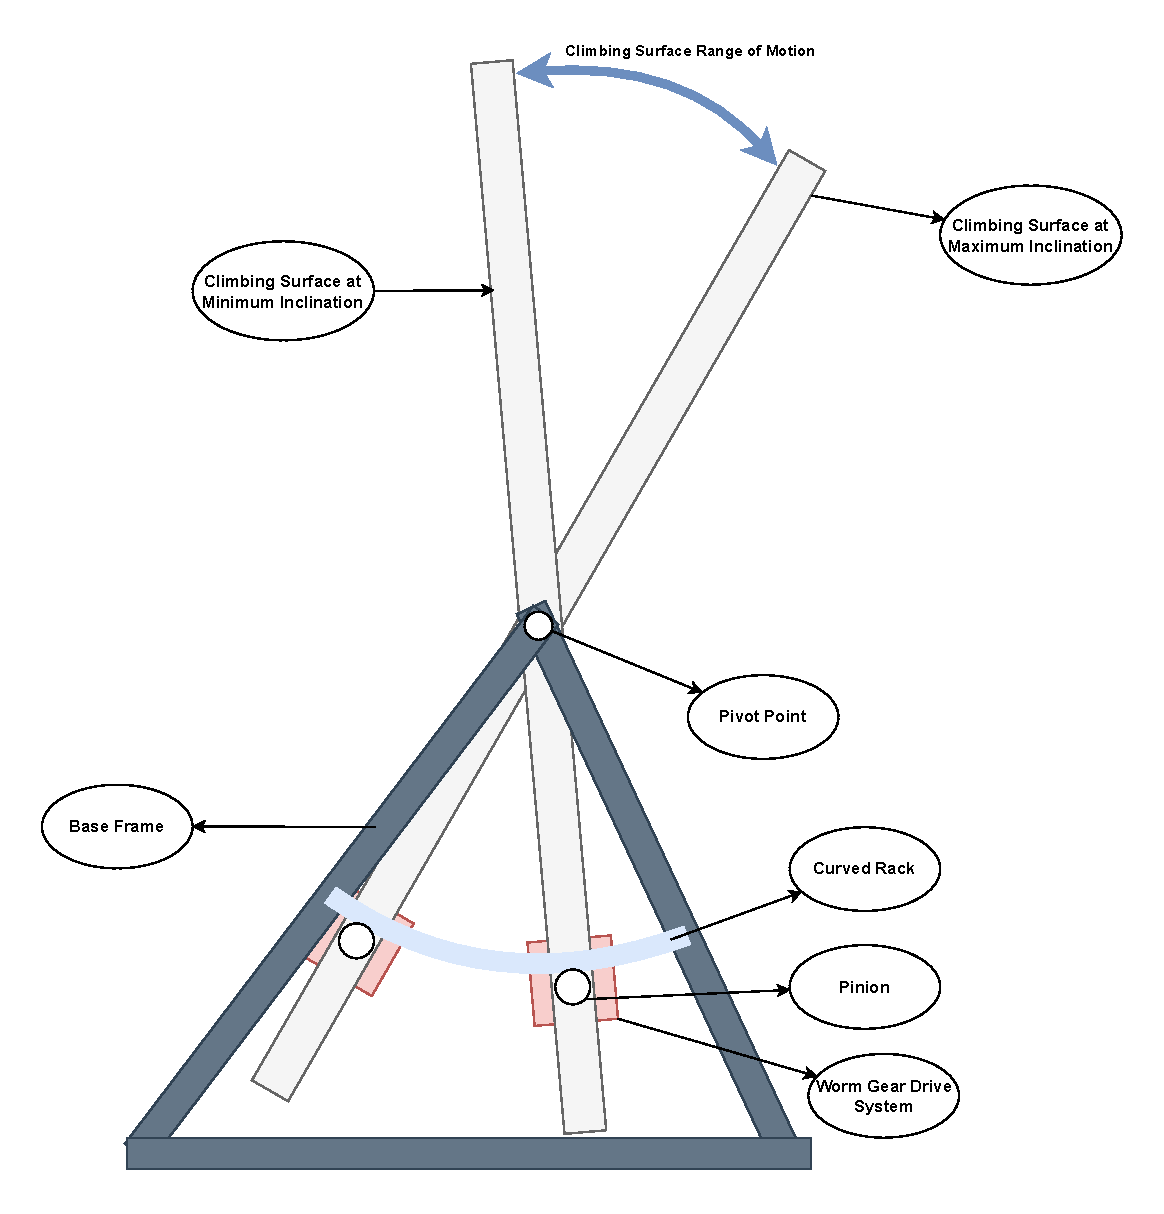
\includegraphics[width=0.6\linewidth]{figs/concept_design/WormGear_Concept.pdf}
    \caption{Worm Gear Automatic Inclination Concept Sketch}
    \label{fig:wormgear-concept}
\end{figure}

\textbf{Advantages:}
\begin{itemize}
    \item Precise control with electronic integration.
    \item Self-locking mechanism enhances safety.
\end{itemize}

\textbf{Disadvantages:}
\begin{itemize}
    \item Moderate cost due to mechanical components and motor.
    \item Increased complexity compared to manual systems.
    \item Increased maintenance as worm gear should be kept aligned and lubricated.
\end{itemize}

\subsubsection{Concept Evaluation and Selection}

\paragraph{Decision Matrix}

\begin{table}[H]
    \centering
    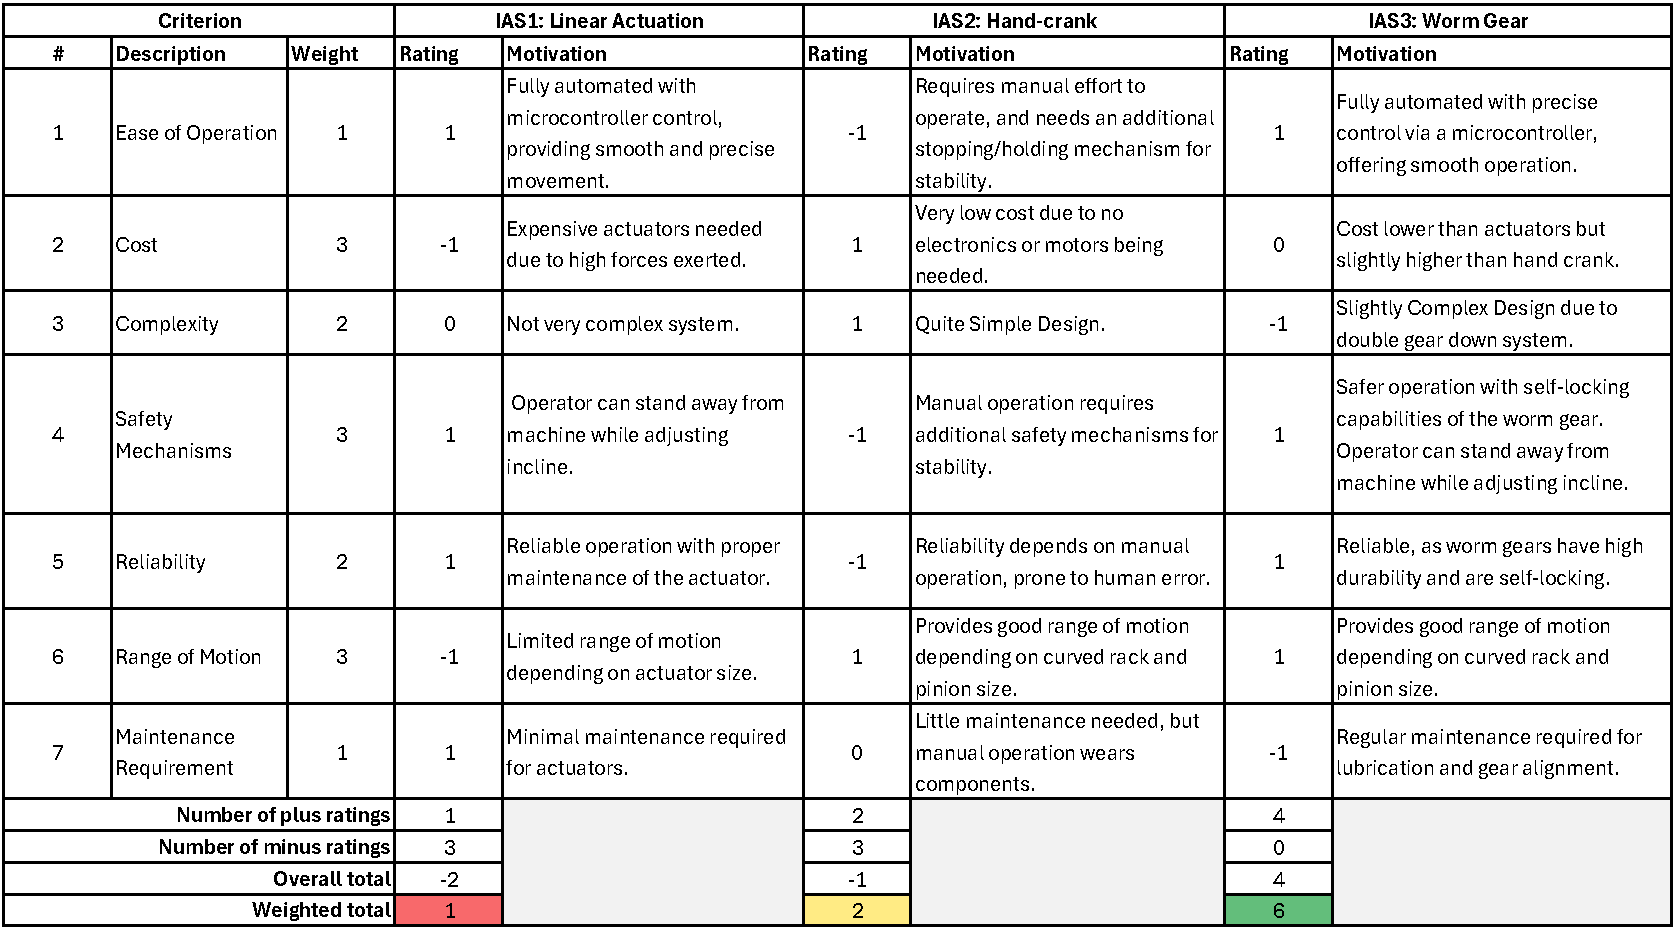
\includegraphics[width=1\linewidth]{tables/IAS_dec_matrix.pdf}
    \caption{Inclination Adjustment System Decision Matrix}
    \label{tab:ias_decision_matrix}
\end{table}

\paragraph{Selection Justification}

Based on the weighted totals, IAS3 (Worm Gear Automatic Inclination) is the preferred concept. It offers precise control, inherent safety due to its self-locking mechanism, and high reliability, all of which are critical for the system's performance and user safety.

\subsection{Braking System}

\subsubsection{Introduction}

The braking system is responsible for controlling the rate of rotation, ensuring the climbing surface moves at a constant and smooth speed. This subsystem addresses FR1 (Speed control and adjustment) and PR1 from the performance requirements.

\subsubsection{Concept Generation}

\paragraph{BS1: Hydraulic Braking System}

This concept uses a hydraulic motor/pump operating in reverse to provide resistance against the rotation. The hydraulic fluid flows through a manually adjustable flow control valve, such as a needle valve, to regulate the speed.

\begin{figure}[H]
    \centering
    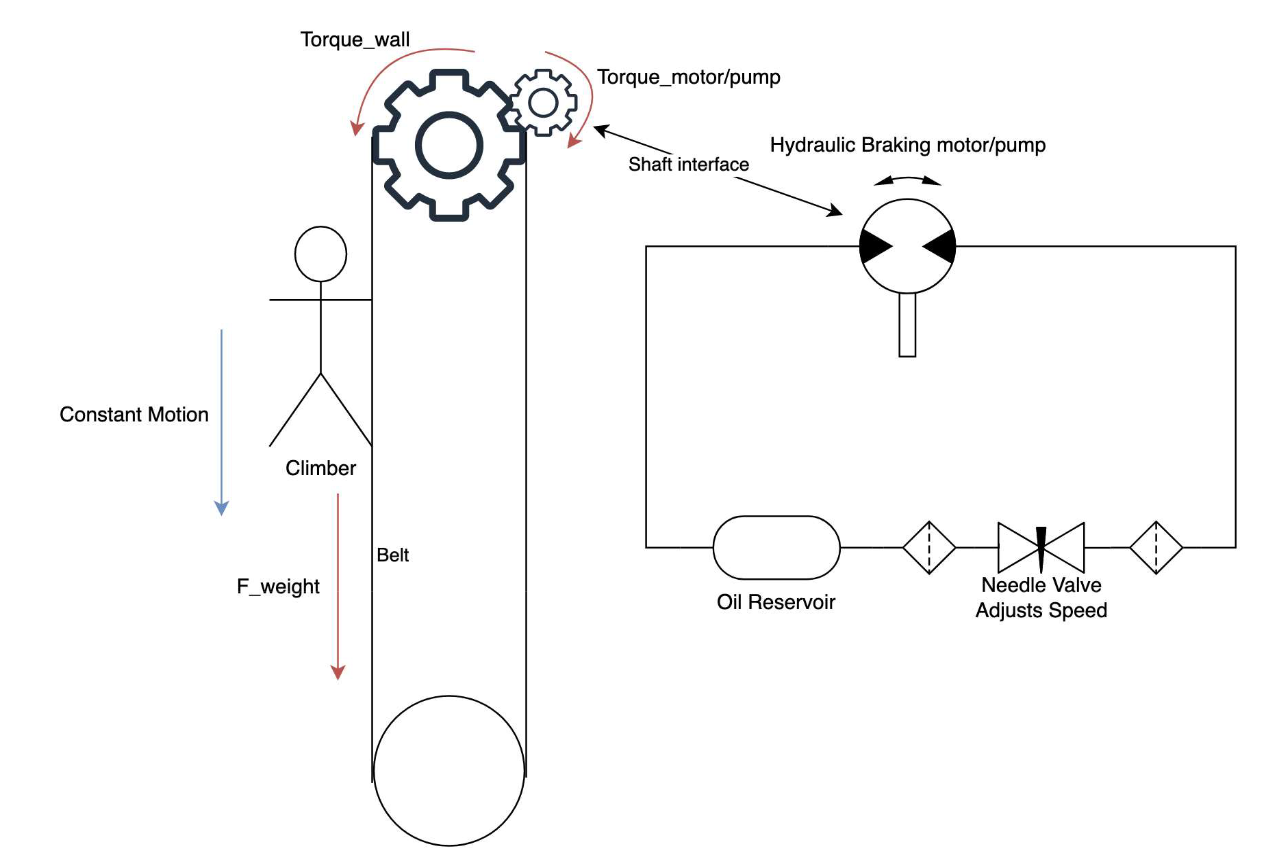
\includegraphics[width=0.6\linewidth]{figs/concept_design/hydraulic_brake_concept.png}
    \caption{Hydraulic Braking System Concept Sketch}
    \label{fig:hydraulic-brake-concept}
\end{figure}

\textbf{Advantages:}
\begin{itemize}
    \item Does not require electronic components to operate.
    \item Robust and durable components.
\end{itemize}

\textbf{Disadvantages:}
\begin{itemize}
    \item Lacks precise speed control (will change speed depending on weight of person).
    \item Manual adjustments required for speed changes.
    \item Potential for leaks and maintenance issues.
    \item Expensive overall system.
\end{itemize}

\paragraph{BS2: Disk Braking System}

This concept adapts an off-the-shelf disk brake system from a motorcycle or mountain bike, controlled automatically to maintain constant rotational speed. Sensors monitor the current speed, and a PID controller adjusts the brake caliper to achieve the desired speed.

\textbf{Advantages:}
\begin{itemize}
    \item Inexpensive and straightforward design.
    \item Utilizes readily available components.
\end{itemize}

\textbf{Disadvantages:}
\begin{itemize}
    \item Potential overheating of brake pads and disk due to continuous use.
    \item Wear and tear leading to frequent maintenance.
    \item Limited precision in speed control.
\end{itemize}

\textbf{Heat Analysis:}

A lumped sum analysis and heat simulation in Fusion 360 were performed to evaluate the thermal performance of the disk brake system (see \ref{calcs:brake-disk-heat}). The results indicated that the brake pads and disk would reach unsafe temperatures after extended use, compromising safety and functionality. This thermal limitation makes BS2 unsuitable for continuous operation required in this application.

\paragraph{BS3: Electromagnetic Braking System}

This concept uses an electric motor and driver to provide electromagnetic braking. The system employs a braking resistor to dissipate the energy generated by the climber-induced rotation.

\textbf{Advantages:}
\begin{itemize}
    \item Precise electronic control over speed irrespective of climber's weight.
    \item Ability to automatically adjust speed to match the speed of the climber.
    \item Smooth and consistent braking performance.
    \item Low maintenance with no physical contact components.
\end{itemize}

\textbf{Disadvantages:}
\begin{itemize}
    \item Slightly higher initial cost due to motor and control systems.
\end{itemize}

\subsubsection{Concept Evaluation and Selection}

\paragraph{Decision Matrix}

\begin{table}[H]
    \centering
    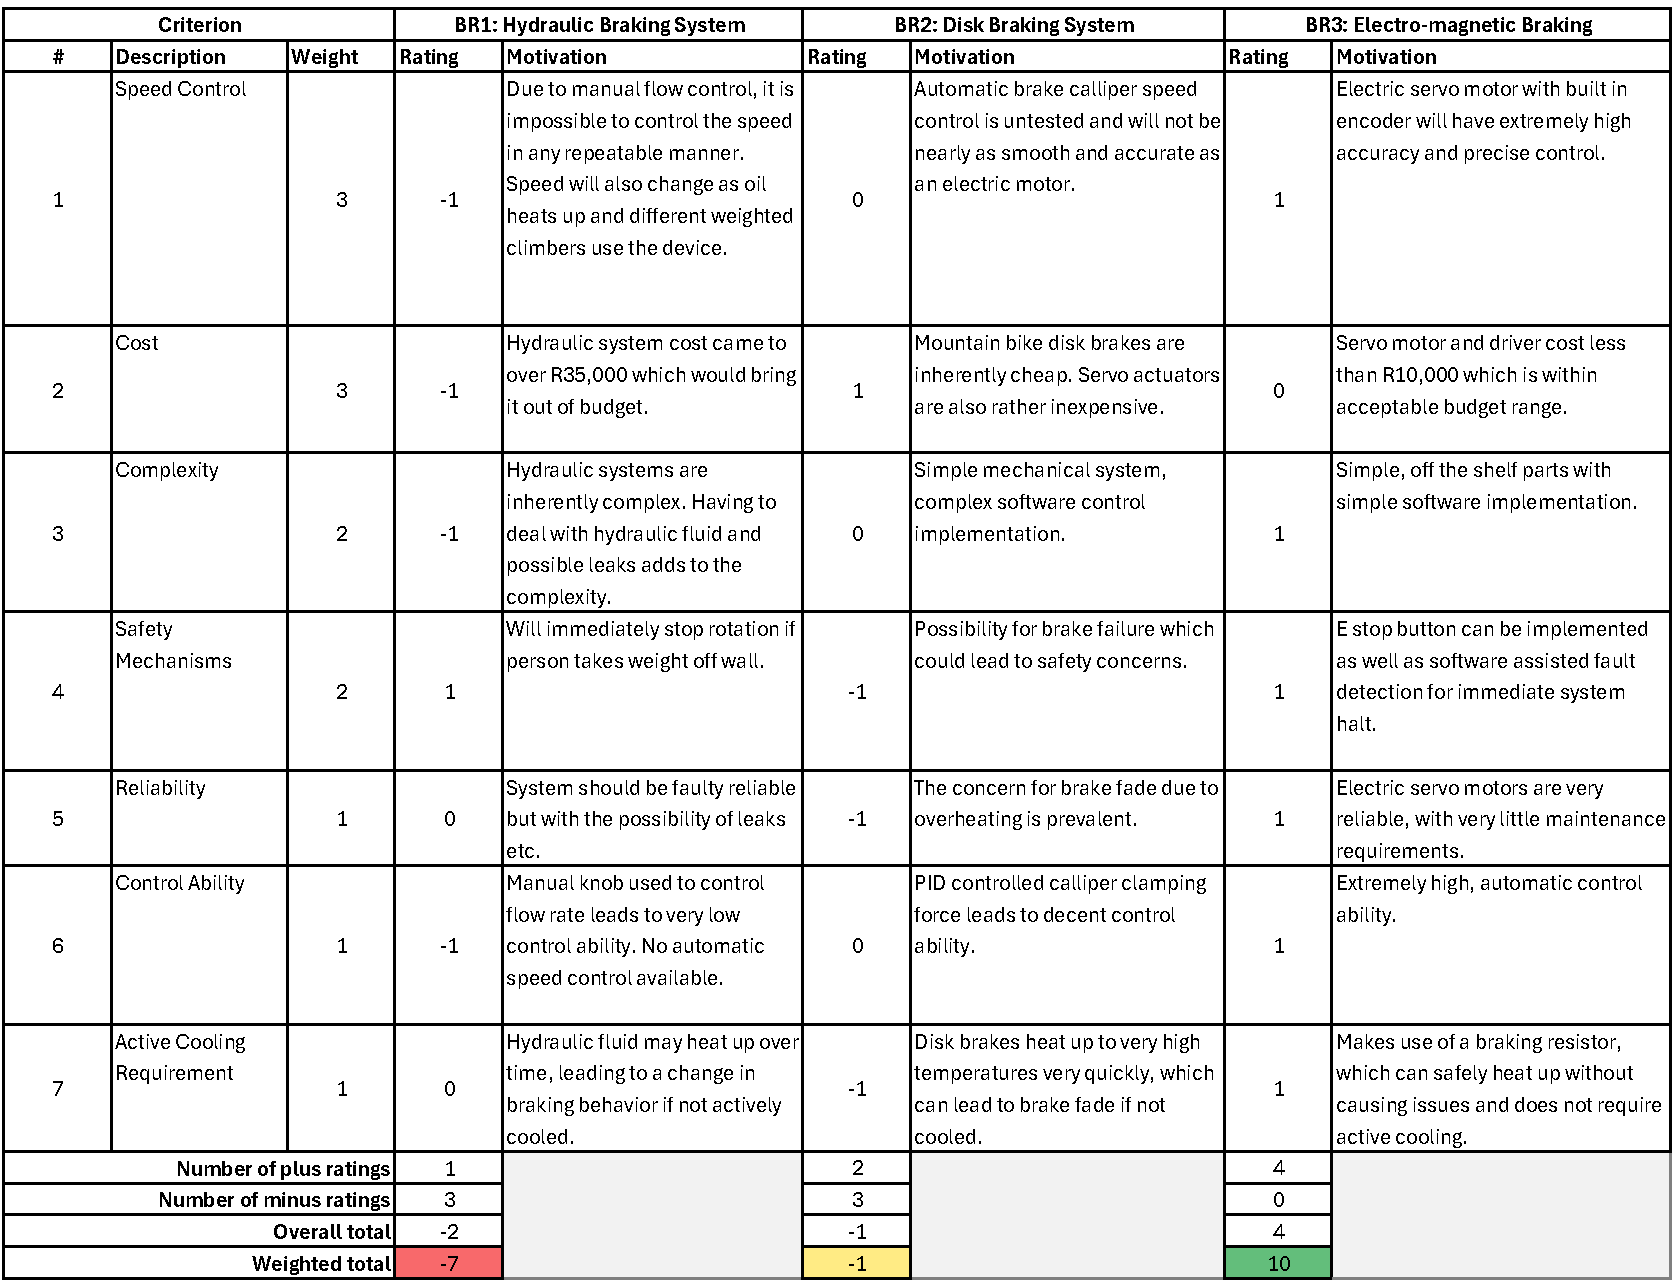
\includegraphics[width=1\linewidth]{tables/BR_dec_matrix.pdf}
    \caption{Braking System Decision Matrix}
    \label{tab:bs_decision_matrix}
\end{table}

\paragraph{Selection Justification}

BS3 (Electromagnetic Braking System) is the preferred concept based on the weighted total. It offers precise control, high safety, low maintenance, and reliability, which are critical factors for the braking system. The higher initial cost is justified by the long-term benefits and performance.

\subsection{Rotating Surface}

\subsubsection{Introduction}

The rotating surface is the central component of the system, providing the physical structure on which climbers ascend. It must securely hold climbing holds and rotate smoothly under load. This subsystem addresses FR5 (Size compliance) and FR6 (Load compliance), along with PR5, PR6, and PR7 from the performance requirements.

\subsubsection{Concept Generation}

\paragraph{RS1: Conveyor Chain Driven Panels}

This concept uses a series of interconnected panels attached to conveyor chains on either side. The chains are looped over sprockets at the top and bottom, driven by the main shafts. The panels form the climbing surface and are pulled along by the chains.

\textbf{Advantages:}
\begin{itemize}
    \item Strong and robust connection between panels and drive system.
    \item Capable of handling high loads from climbers.
    \item Reliable operation.
\end{itemize}

\textbf{Disadvantages:}
\begin{itemize}
    \item Higher cost due to chains and sprockets.
    \item Increased weight of the system.
    \item Requires precise alignment to prevent chain derailment.
\end{itemize}

\paragraph{RS2: Rubber Conveyor Belt Panels}

This concept employs a continuous rubber conveyor belt with climbing holds attached directly to the belt or to panels affixed to the belt. The belt wraps around drums or rollers at the top and bottom, driven by the main shafts.

\textbf{Advantages:}
\begin{itemize}
    \item Simpler construction with fewer moving parts.
    \item Potentially lower cost than chain systems.
    \item Smooth and continuous climbing surface.
\end{itemize}

\textbf{Disadvantages:}
\begin{itemize}
    \item Limited load capacity; may not handle high loads well.
    \item Difficulty in attaching and securing climbing holds.
    \item Potential for belt stretching and slippage over time.
\end{itemize}

\subsubsection{Concept Evaluation and Selection}

\paragraph{Decision Matrix}

\begin{table}[H]
    \centering
    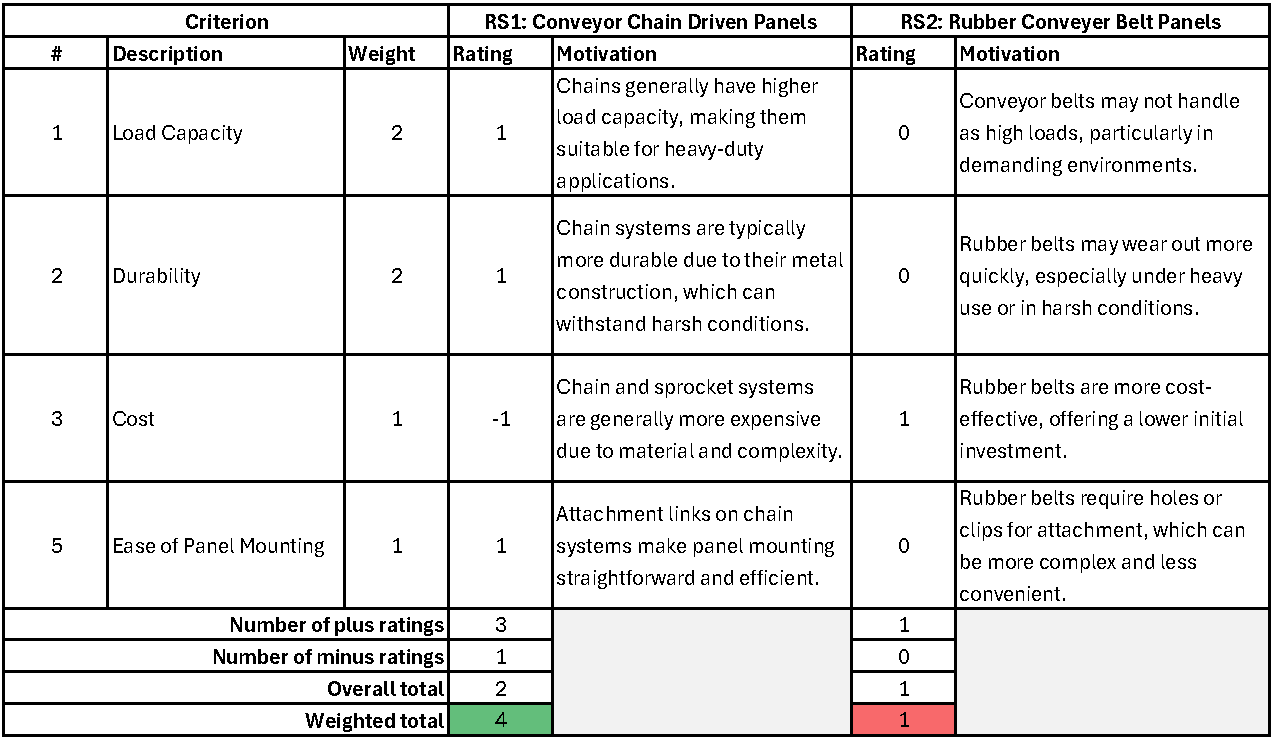
\includegraphics[width=1\linewidth]{tables/RS_dec_matrix.pdf}
    \caption{Rotating Surface Decision Matrix}
    \label{tab:rs_decision_matrix}
\end{table}

\paragraph{Selection Justification}

RS1 (Conveyor Chain-Driven Panels) is the preferred concept due to its superior load capacity and durability, which are essential for supporting climbers safely. While it has higher costs and complexity, these drawbacks are offset by the benefits in performance and safety.

\section{Conclusion}

Through a rigorous concept development and evaluation process, the preferred concepts for each of the main subsystems have been selected:

\begin{itemize}
    \item \textbf{Inclination Adjustment System:} IAS3 (Worm Gear Automatic Inclination)
    \item \textbf{Braking System:} BS3 (Electromagnetic Braking System)
    \item \textbf{Rotating Surface:} RS1 (Conveyor Chain-Driven Panels)
\end{itemize}

These selections are justified based on their performance against the defined criteria, alignment with stakeholder and engineering requirements, and their ability to integrate effectively within the overall system design.

Future work will focus on detailed design, including precise calculations, simulations, and integration of the control and safety systems.

\chapter{Final Design}
\label{chap:detailed_design}

This chapter presents the final design process for the rotating climbing wall, focusing on the key subsystems, as well as the integration of these systems. Each main component was selected and designed to meet the requirements set out in Chapter \ref{chap:concept_design}. Structural verification was carried out through both analytical and simulation-based approaches.

Due to the complex nature of verifying stress and displacement in many of the mechanical systems, the native Finite Element Method (FEM) package in Autodesk Fusion 360 was employed to perform static simulations. To ensure the correct usage of the package, a verification process was conducted (as detailed in Appendix~\ref{appx:FEM-verification}). A simulation was performed on a simple test case, where the FEM package overestimated stress by just over 5\% and displacement within 0.6\%. These results provided confidence to utilize the package for more complex simulations.

\section{Main Dimensions}

As discussed in the technology review (see Chapter~\ref{chap:technology_review}), typical market products for rotating climbing walls vary in size. The largest, the Treadwall Max6/12, features a climbing surface measuring 1.83\,m in width and 3.1\,m in height, while the smallest, the Treadwall Kore4/11, measures 1.22\,m in width and 2.75\,m in height.

For this design, a slightly smaller design was chosen, with dimensions of approximately 1.1\,m in width and 2.5\,m in height. This size ensures that the wall is not so small that it becomes ineffective for training or unsuitable for taller climbers, yet not so large that it significantly increases the development cost of the prototype.

All major components of the design—including shaft widths, upright beams, crossbeams, and other structural elements—were guided by these chosen dimensions.

\section{Inclination Adjustment System}

The inclination adjustment system employs a compound gear reduction mechanism to achieve precise control over the tilting angle of the climbing wall. The primary reduction stage consists of two large sector gears (curved racks) secured to the base frame and two small pinions mounted on the ends of the tilting shaft. This shaft is connected to the tilting frame via bearings and brackets to ensure smooth rotation. The torque required to drive the pinions along the sector gears is generated by a custom-designed worm gear assembly, actuated by a stepper motor. This worm gear assembly is affixed to the lower crossbeam of the tilting frame.

\subsection{Sector Gear and Pinion Design}

The sector gears have a pitch radius of 852\,mm, measured from the pivot point of the tilting mechanism. This dimension was selected based on the placement of the lower crossbeam and the worm gear assembly. The pinion gears have a pitch radius of 24\,mm, optimizing the gear ratio to enhance torque transmission while ensuring proper meshing with the sector gears.

Both the sector gears and pinions are fabricated via laser cutting from 6\,mm mild steel, chosen for its stiffness and manufacturability. Initially, the gear teeth were designed to oriented on the upper edge of the sector gears; however, they were repositioned to the lower edge to improve safety by reducing the risk of foreign objects becoming caught in the gear mesh.\\

The sector gears are securely mounted to the main frame, which has been designed for structural stability (wide legs to avoid tipping). This configuration permits a broader range of tilt angles, from $-46^\circ$ to $+30^\circ$, exceeding the requirements PR2 and PR3 specified in Section~\ref{tab:performance-requirements}. The extended range was achieved without incurring significant additional complexity or costs.\\

Given the critical role of the pinions in torque transmission, stress calculations were performed (see Appendix~\ref{calcs:pinion-SF}) to verify their structural integrity under load. Using the Lewis equation for gear tooth bending stress from \cite{budynas2015shigley}, the estimated bending stress was calculated to be 5.83\,MPa. This results in a safety factor of 42.88, based on the yield strength of the material. These results demonstrate that the pinions operate well within the acceptable stress limits, ensuring reliable performance under operational loads.

\subsection{Worm Gear Drive Assembly}
The worm gear drive assembly must be engineered to withstand substantial loads, as it maintains the entire system at the desired incline angle during operation. A mild steel shaft of 8mm thickness was chosen to transfer the torque from the stepper motor to the worm motor. The assembly comprises four critical components that must be robustly designed to prevent failure:

\begin{enumerate}
    \item \textbf{Worm Gear Set:} Converts rotational motion from the stepper motor into the torque required to drive the tilting mechanism.
    \item \textbf{Thrust Bearings:} Transfer axial force from worm gear to mounting brackets, taking axial force from pillow block bearings.
    \item \textbf{Mounting Brackets:} Secure the worm gear assembly to the tilting frame and ensure alignment of the components.
    \item \textbf{Stepper Motor:} Provides the necessary rotational input to the worm gear for inclination adjustment.
\end{enumerate}

\subsubsection{Worm Gear Set}

The worm gear set consists of a stainless steel worm (helical screw) and a brass worm wheel (helical gear). Ideally a more durable material would have been selected instead of brass, but the set was the only available worm set found that met the sizing specifications. The worm, coupled to a secondary shaft which is coupled to the stepper motor via flexible coupling, engages with the worm wheel, achieving a 28:1 reduction ratio and exhibiting self-locking properties. This design ensures that the system remains stationary when not being adjusted, providing safety and stability. The self-locking feature is critical, as it prevents back-driving, ensuring that the inclination angle remains fixed under load without the need for additional braking mechanisms. The brass worm wheel was identified as the critical component in this system and calculations were performed (see Appendix \ref{calcs:incline-system}) with a resulting gear tooth stress of 34.5MPa and safety factor of 1.3 which is slightly low, but acceptable for a prototype.

\subsubsection{Thrust Bearings}
8mm thrust bearings were selected to take the axial load of the worm gear and transfer it straight into the mounting brackets and not the shaft. The calculations performed in Appendix \ref{calcs:incline-system} yield maximum estimated force of 1.75KN with a safety factor of 1.7.


\subsubsection{Mounting Brackets}

The mounting brackets are laser-cut and bent mild steel for their relatively low price and high strength, as well as ease of manufacturing. These brackets ensure proper alignment of the worm and worm wheel and secure the assembly to the lower crossbeam of the tilting frame. Slots were designed instead of holes to allow for further alignment of the assembly. Figure \ref{fig:FEM-incline-brackets} shows the Finite Element Analysis (FEA) was performed to validate the structural integrity of the brackets under operational loads, safety factor of 1.2 (refer to Appendix~\ref{calcs:worm-bracket-fem}).

\begin{figure}[H]
    \centering
    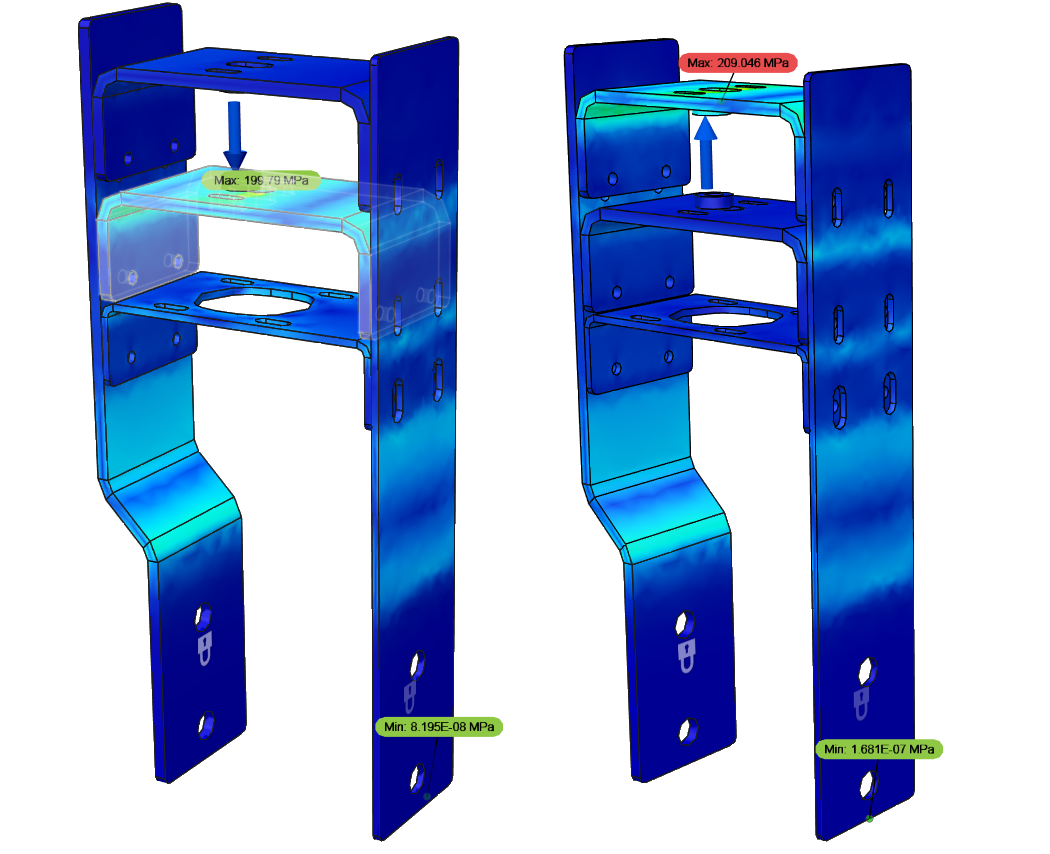
\includegraphics[width=0.6\linewidth]{figs/FEM/incline-braket.png}
    \caption{FEM Analysis Results on Worm Gear Bracket System}
    \label{fig:FEM-incline-brackets}
\end{figure}

\subsubsection{Stepper Motor Selection}
To determine the appropriate motor for driving the inclination adjustment system, calculations were performed (see Appendix~\ref{calcs:stepper-motor}) to establish the required torque and speed. The torque required was calculated to be 1.87\,Nm, while speed was not a critical factor since tilt speed was not specified as a requirement. 

A Nema 23 stepper motor, with an output torque of 2\,Nm, was selected as it met the torque requirements. Additionally, it was available in stock at the mechatronics store, and stepper motors are both cost-effective and offer precise control, making it an ideal choice for this application.

\subsection{Shaft Selection}
Following FEM simulations (see Appendix~\ref{calcs:incline-system}), which used the maximum expected torque on the shaft (see Section~\ref{calcs:incline-system}) as input, a 16\,mm mild steel shaft was selected. The analysis showed a safety factor of 1.54 and a displacement of 0.746\,mm under the given load, both of which were deemed acceptable for the prototype.

The shaft is supported by three UCFL203FKD/ISO flange bearings, selected for their compact size, affordability, and static load rating of 6.65\,kN found in \cite{ntn_bearings2024}. Given the non-critical nature of these components in this application, it is assumed that the selected bearings can adequately handle the expected load.

\begin{figure}[H]
    \centering
    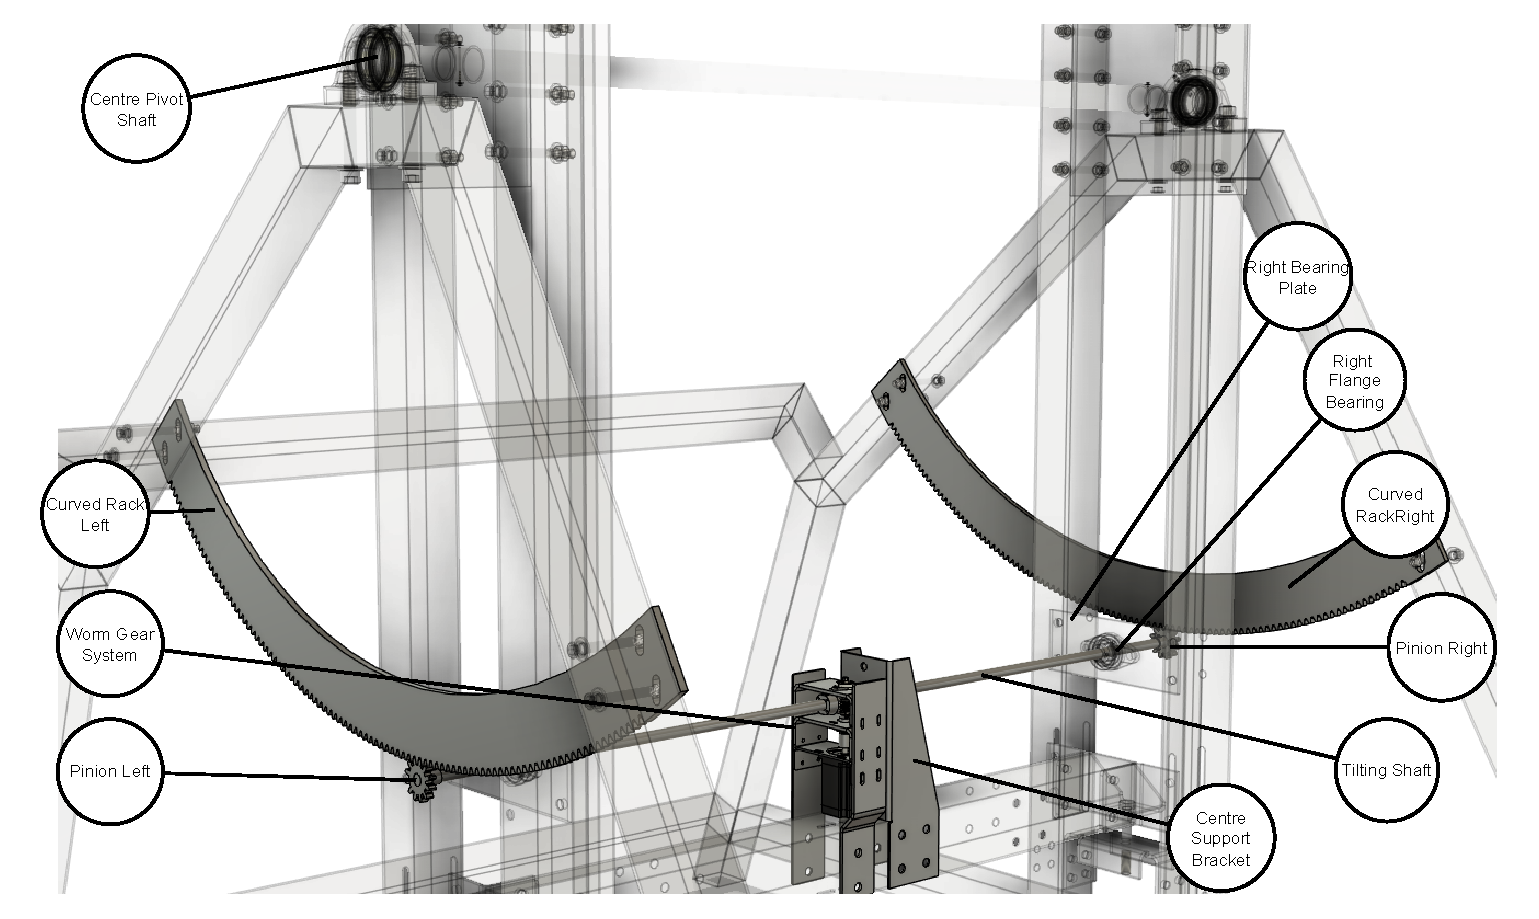
\includegraphics[width=1\linewidth]{figs/final_design/Incline_subsystem_CAD-1.pdf}
    \caption{Sector Gear and Pinion Final Design CAD Representation}
    \label{fig:sector-gear-pinion-cad}
\end{figure}

\begin{figure}[H]
    \centering
    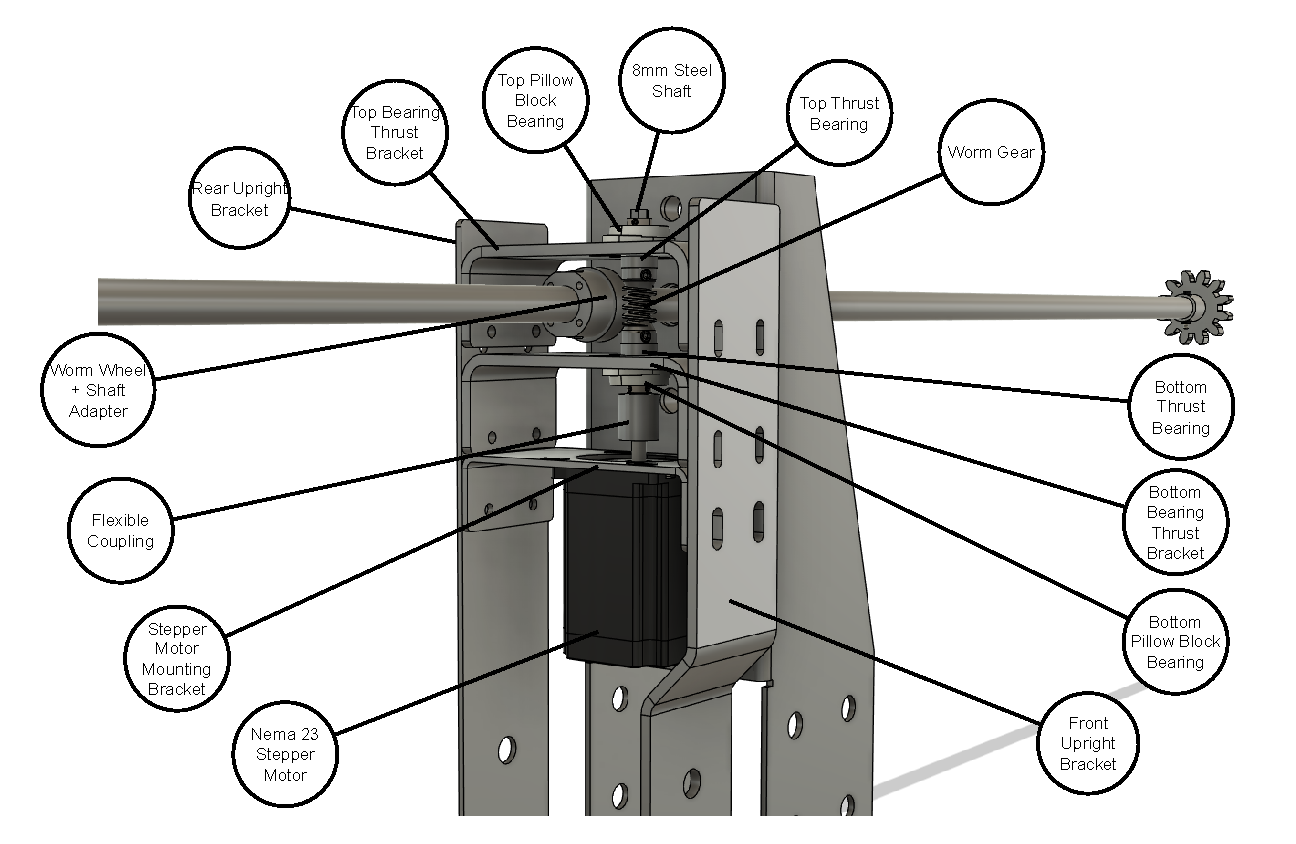
\includegraphics[width=1\linewidth]{figs/final_design/wormgear_assembly_CAD.pdf}
    \caption{Worm Gear Drive Assembly Final Design CAD Representation}
    \label{fig:worm-gear-drive-cad}
\end{figure}


\section{Braking System}

The braking system was designed to include an active braking component secured to the top crossbeam. Due to space limitations, the bottom crossbeam was reserved for the tilting system, necessitating the placement of the braking mechanism on the top crossbeam. This subsystem utilizes a pulley-driven AC servomotor for electromagnetic braking, with the main driven shaft mounted through a series of three deep groove flange ball bearings. These bearings are \textbf{Koyo UCF205 Flange unit bearings}, chosen for their ability to handle the calculated loads and ease of mounting. The bearings are mounted via laser-cut and bent sheet metal brackets to the top crossbeam. Figure~\ref{fig:brake-system-final-design} shows the final braking system CAD representation.

\subsection{Main Shafts}

To maintain a constant speed on the rotating surface, a braking torque of 210\,Nm was required on the top main shaft. This calculation was based on a climber’s weight estimate of 1400\,N, providing an added safety margin (excluding friction). The downward force on each sprocket of the shaft was calculated to be 1.11\,kN (calculations can be found in Appendix \ref{calcs:main_braking_shaft}).

Bright mild steel was selected as the shaft material due to its cost-effectiveness and strong mechanical properties. Finite Element Analysis (FEA) was performed in Autodesk Fusion 360 on both 30\,mm and 25\,mm diameter solid shafts, yielding safety factors of 3.47 and 2.24, respectively. Based on these results, a 25\,mm solid bright steel shaft was chosen for both the top and bottom main shafts.

Figure~\ref{fig:FEM-mainshaft} displays the FEA results for the shaft, revealing a stress concentration toward the middle. To address this, an extra Koyo UCF205 bearing was placed near the middle of the shaft to provide additional support.

\begin{figure}[h]
    \centering
    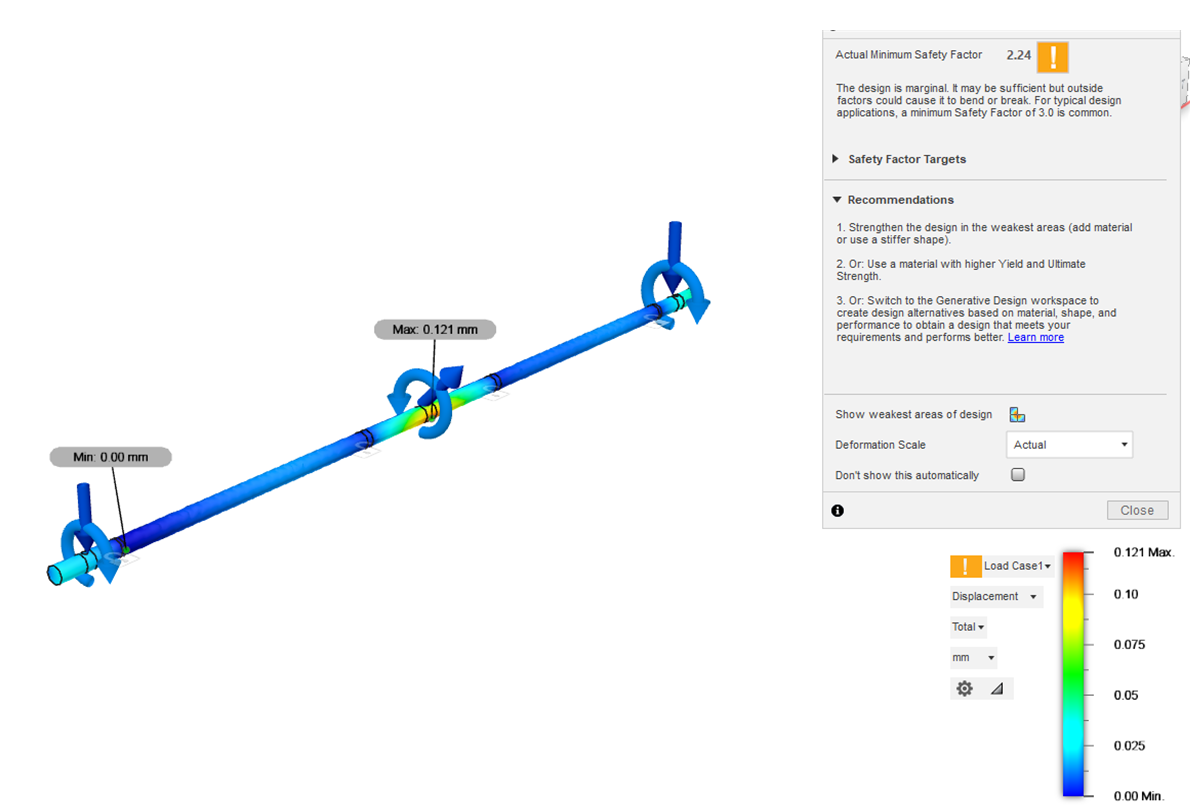
\includegraphics[width=0.8\linewidth]{figs/final_design/FEMShaft.png}
    \caption{FEA Results of 25\,mm Diameter Main Shaft}
    \label{fig:FEM-mainshaft}
\end{figure}

\subsection{Brackets and Bearings}

The brackets were designed to be laser-cut and bent from mild steel due to its favorable cost-to-strength ratio. Stainless steel was considered for its extra strength and corrosion resistance but was ruled out since the wall will be placed indoors, and mild steel can be painted to prevent rust. Due to the complexity of the bracket shapes, FEA was performed using 6\,mm thick mild steel, simulating the worst-case scenario of holding the entire weight of the climber, panels, and chain tension. The safety factor at a vertical wall inclination was 5.93, while at a $-45^\circ$ inclination, the safety factor was 1.33. Although slightly low, the high load estimate and prototype nature of the wall justify this. Figure~\ref{fig:FEM-bracket} shows the FEA results of the bracket at a $45^\circ$ incline. Further calculations can be found in Appendix \ref{calcs:brackets_bearings}.

\begin{figure}[ht]
    \centering
    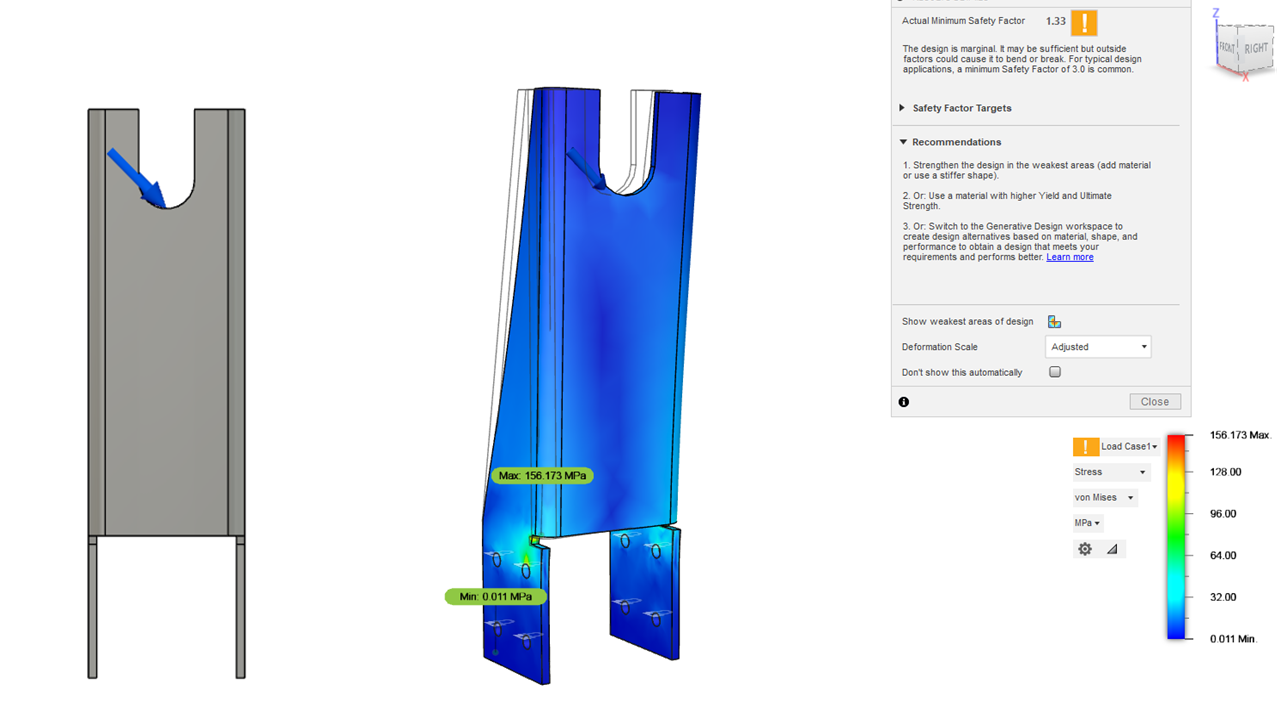
\includegraphics[width=0.8\linewidth]{figs/final_design/FEMBracket45.png}
    \caption{FEA Results of Bracket at $45^\circ$ Incline}
    \label{fig:FEM-bracket}
\end{figure}

\subsection{Motor and Belt Drive System}

The top shaft must resist approximately 50\,Nm of torque, factoring in friction losses of around 61\,Nm (for a lighter climber weight of 90\,kg). Calculations for this are found in Appendix \ref{calcs:motor_belt}. This system prioritizes cost control while maintaining sufficient safety.

An AC servomotor and driver system was selected; the \textbf{MiGE 130ST-M10010} motor was chosen for its suitable specifications (see Table~\ref{tab:motor_specs}). A basic calculation was performed to determine the necessary torque reduction ratio after accounting for mechanical losses.

\begin{table}[H]
    \centering
    \begin{tabular}{|l|c|}
        \hline
        \textbf{Motor Model} & 130ST-M10010 \\
        \hline
        Rated Power (kW) & 1.0 \\
        \hline
        Rated Voltage (V) & 220 \\
        \hline
        Rated Current (A) & 4.5 \\
        \hline
        Rated Speed (rpm) & 1000 \\
        \hline
        Holding Torque (Nm) & 10 \\
        \hline
        Peak Torque (Nm) & 20 \\
        \hline
        Voltage Constant (V/krpm) & 140 \\
        \hline
        Torque Coefficient (Nm/A) & 2.2 \\
        \hline
        Rotor Inertia (kg$\cdot$m$^2$) & $1.94 \times 10^{-3}$ \\
        \hline
        Line-Line Resistance ($\Omega$) & 2.7 \\
        \hline
        Line-Line Inductance (mH) & 8.8 \\
        \hline
        Mechanical Time Constant (ms) & 3.26 \\
        \hline
        Weight (kg) & 11.5 \\
        \hline
    \end{tabular}
    \caption{MiGE Motor Specifications}
    \label{tab:motor_specs}
\end{table}

With a peak holding torque of 20\,Nm, a continuous torque of 10\,Nm, and a power rating of 1\,kW, this motor is well-suited for the application when paired with the appropriate gear reduction system.

\subsubsection*{Torque Reduction Ratio Calculation}

The required torque at the shaft is:

\[
T_{\text{shaft}} = 45.44\ \text{Nm}
\]

The motor's continuous torque is:

\[
T_{\text{motor}} = 10\ \text{Nm}
\]

Therefore, the necessary gear reduction ratio (\( R \)) is:

\[
R = \frac{T_{\text{shaft}}}{T_{\text{motor}}} = \frac{45.44\ \text{Nm}}{10\ \text{Nm}} = 4.544
\]

A gear reduction ratio of approximately 5:1 is required to meet the torque demands. The SKF Power Transmission Belt Software \cite{SKF_BeltDriveTool} was used to select an M5 timing belt and a 90-tooth to 18-tooth pulley system, providing the needed 5:1 gear ratio. This results in a continuous torque of 50\,Nm and a maximum torque of 100\,Nm on the main shaft, meeting the main shaft torque and speed criteria. Belt calculations are found in Appendix \ref{calcs:motor_belt}.

\subsection{Braking Resistor}

To dissipate the energy generated by the motor due to the climber's weight and resulting rotation, a braking resistor is employed. The resistor is connected to the designated output pins on the motor driver, with the required values calculated in Appendix \ref{calcs:braking_resistor}. Finding a braking resistor with exactly these specifications is challenging, so the braking resistor that was purchased was overspecified. Table~\ref{tab:braking-resistor-specs} shows the calculated values and the specifications of the selected resistor.

\begin{table}[H]
    \centering
    \begin{tabular}{|l|c|c|}
        \hline
        \textbf{Specification} & \textbf{Calculated Value} & \textbf{Selected Resistor Value} \\
        \hline
        Power (W) & 227.2 & 1000 \\
        \hline
        Resistance ($\Omega$) & 2.19 & 16 \\
        \hline
    \end{tabular}
    \caption{Braking Resistor Specifications}
    \label{tab:braking-resistor-specs}
\end{table}

Figure~\ref{fig:brake-system-final-design} illustrates the final CAD design of the braking system.

\begin{figure}[H]
    \centering
    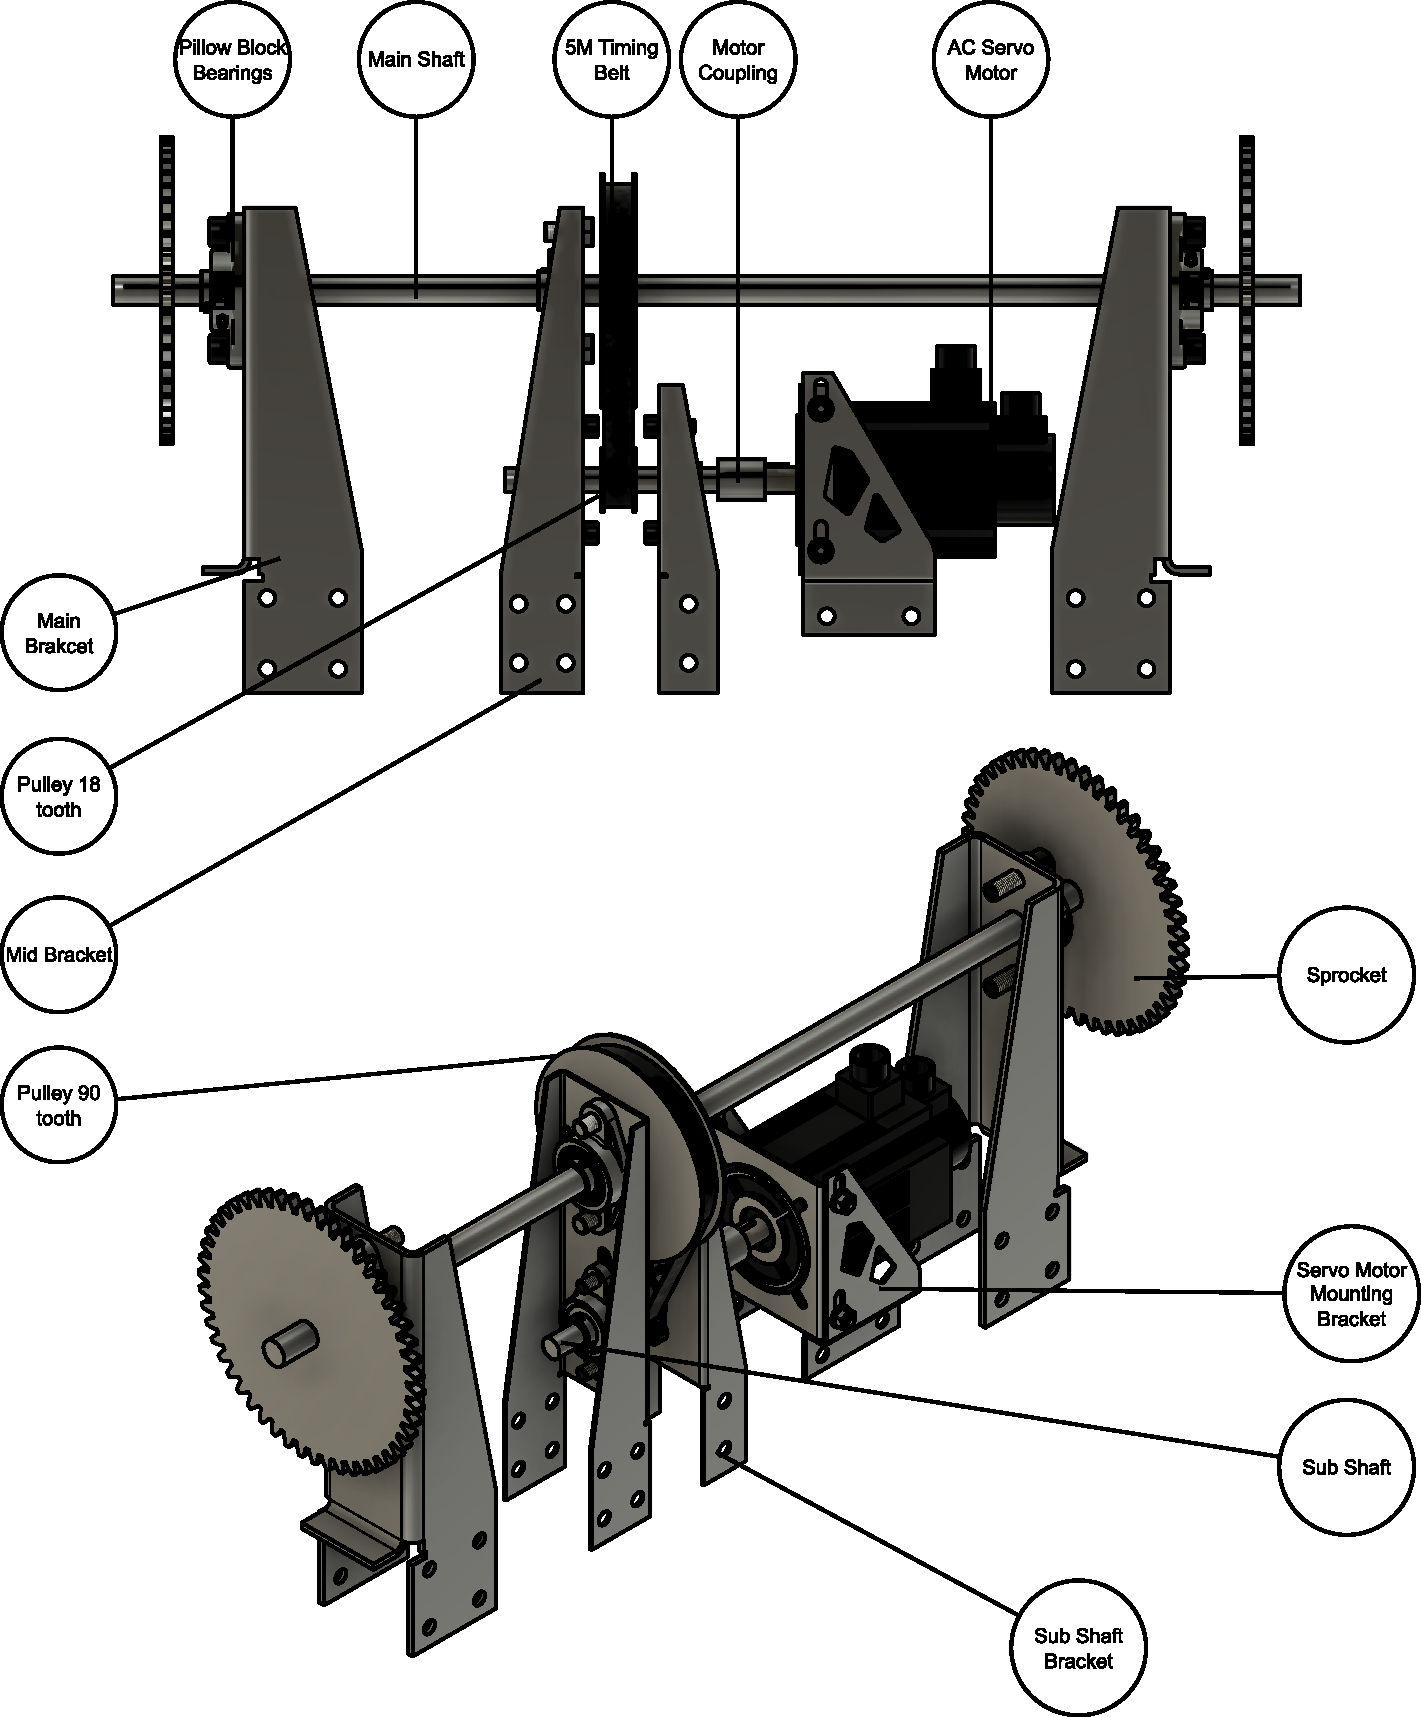
\includegraphics[width=0.8\linewidth]{figs/final_design/BrakingSyst.pdf}
    \caption{Braking System Final CAD Design}
    \label{fig:brake-system-final-design}
\end{figure}

\section{Rotating Surface Final Design}
The rotating surface consists of a pair of conveyor chains wrapped around the sprockets. The top sprockets are connected to the braking system, while the bottom sprockets rotate freely. Forty-one wooden panels are attached to the chain to form the climbing surface.

\subsection{Conveyor Chain Selection}
To determine the appropriate chain, calculations were performed (see Appendix~\ref{calcs:chain}) to find the required length and maximum tension. A pair of standard roller chains were sourced from West Cape Bearings, modified by replacing every sixth link with an attachment link. This modification resulted in a spacing of 153\,mm between the attachment links.

\subsection{Panel Design}
To minimize costs, 21\,mm shutterply (the most affordable grade of plywood) from Timbuild City Stellenbosch was chosen as the primary panel material. Forty-one panels, each measuring 140\,mm x 1664\,mm, were cut from the plywood sheets. For added rigidity, a 32\,mm x 44\,mm pine brace was fastened to the back of each panel.

FEM analysis was performed to ensure the strength of this design under worst-case conditions, with the assumption of a 100\,kg person hanging with their entire weight concentrated in the middle of a single panel at a 45-degree incline. As shown in Figure~\ref{fig:FEM-panel}, the maximum stress is compressive on the pine support. Pine has a compressive strength along the grain of approximately 6.20\,MPa \cite{matweb2024pine}. Using this value, the safety factor is calculated as follows:

\[
\text{SF} = \frac{\sigma_{\text{yield}}}{\sigma_{\text{max}}} = \frac{6.20 \, \text{MPa}}{2.10 \, \text{MPa}} \approx 2.95
\]

This provides a safety factor of approximately 2.95, which confirms the strength of the design. The panel deflection, which was calculated to be nearly 20\,mm, will be further verified in the load testing described in Section~\ref{sec:incline-load-test}.

\begin{figure}[H]
    \centering
    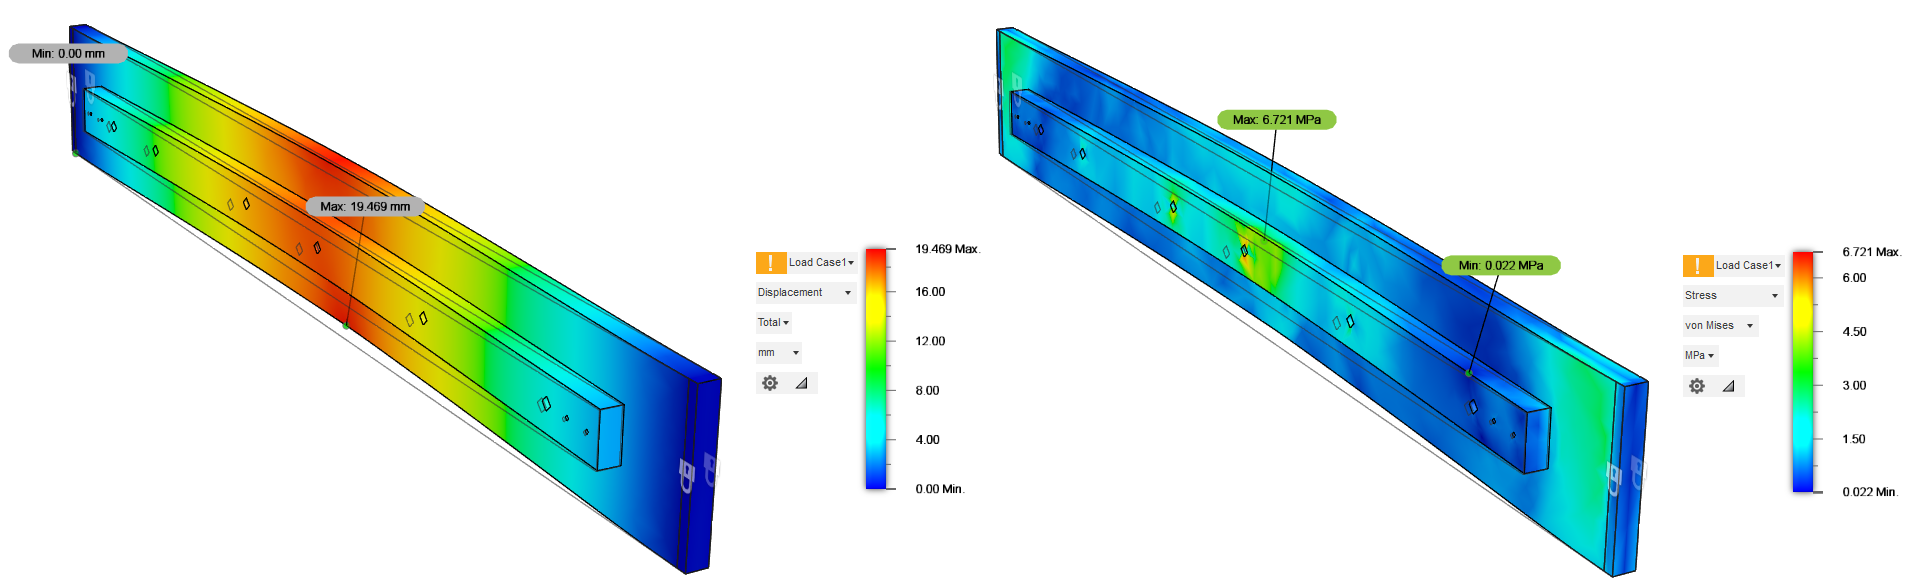
\includegraphics[width=1\linewidth]{figs/FEM/FEM-panel.png}
    \caption{FEM Analysis of Panel Assembly showing displacement (left) and stress (right)}
    \label{fig:FEM-panel}
\end{figure}





\section{Integration, Frame and Final Assembly}

To integrate the various sub-systems into a cohesive working system, two frames were designed. The base frame serves as a stable platform, around which the rest of the system is mounted, centered on a pivot point. This pivot point utilizes a 40\,mm mild steel solid shaft, which passes through two UCP208 KOYO pillow block bearings. These bearings were chosen for their straightforward mounting capabilities, allowing them to be affixed directly to the base frame.

The base frame was fabricated from 76x76x2\,mm mild steel square tubing, selected for its cost-effectiveness. The upright frame, providing structural support for the rotating system, was assembled using 6\,mm laser-cut and bent mild steel brackets. Each side of the upright frame features two 76x76x2\,mm vertical supports, while the crossbeams were made from 100x100x2\,mm mild steel square tubes to enhance rigidity.

FEM analysis was conducted on the frame to verify its structural integrity under the expected loads. This analysis is detailed in Appendix \ref{calcs:FEM-frame}.

A chain tensioning mechanism was designed to simplify the process of adjusting chain tension by tightening a single bolt on each chain. This mechanism is illustrated in Figure \ref{fig:chain-tensioning-CAD}, while Figure \ref{fig:chain-tensioning-photo} provides a side view into the inner workings of the wall. This view reveals the chain tensioning system, the worm gear inclination system, and the mounting of brackets to the chain.

\begin{figure}[H]
    \centering
    \begin{minipage}[b]{0.55\linewidth}
        \centering
        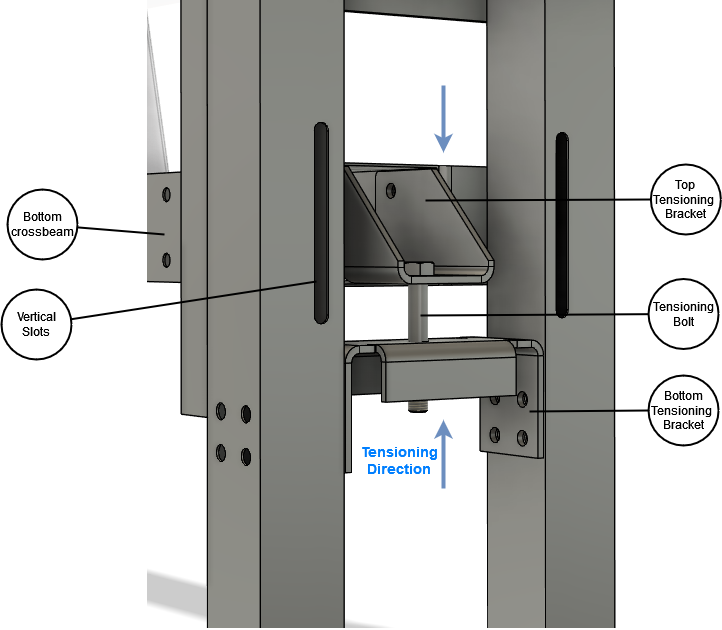
\includegraphics[width=\linewidth]{figs/final_design/chain-tension-CAD.png}
        \caption{CAD model of the chain tensioning mechanism.}
        \label{fig:chain-tensioning-CAD}
    \end{minipage}
    \hspace{0.05\linewidth}
    \begin{minipage}[b]{0.35\linewidth}
        \centering
        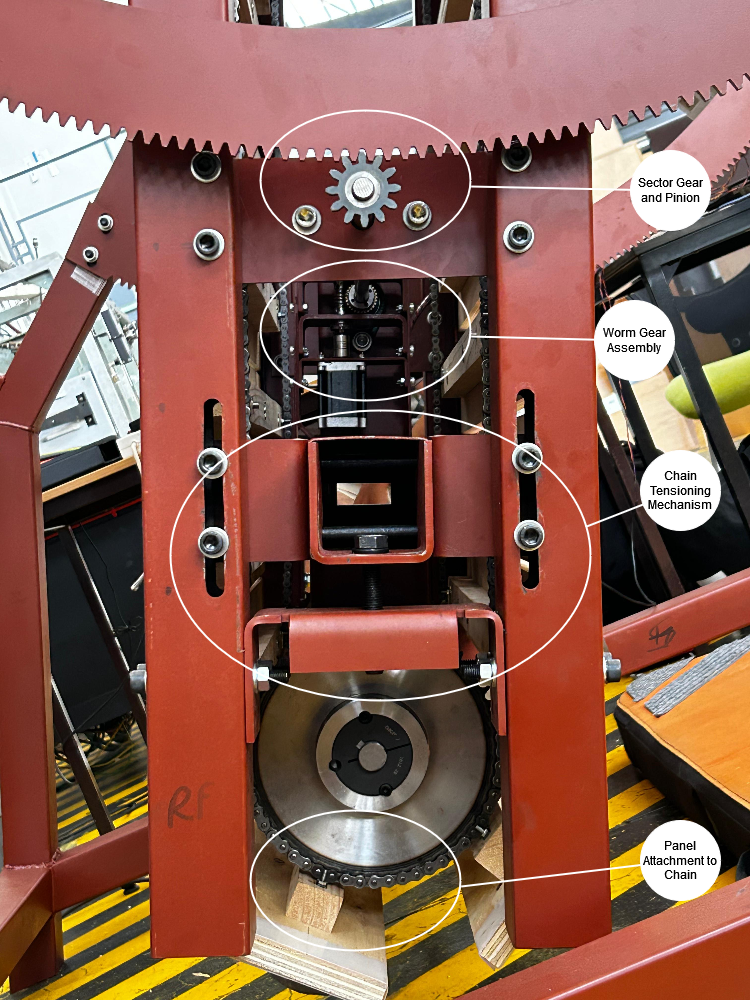
\includegraphics[width=\linewidth]{figs/final_design/side-mechanisms-photo.png}
        \caption{Side view showing inner workings.}
        \label{fig:chain-tensioning-photo}
    \end{minipage}
\end{figure}



Based on CAD simulations, the estimated weight of the upright section is approximately 320\,kg, with the lower frame contributing an additional 79\,kg. Thus, the total system weight is estimated at:

\[
\text{Total Weight} = 320\,\text{kg} + 79\,\text{kg} = 399\,\text{kg}
\]

The final assembly ensures that all components are securely mounted and supported, with structural integrity confirmed through both FEM analysis and physical design validation.

The final CAD assembly, shown in Figure \ref{fig:full-assembly-final-design}, illustrates the system with one panel removed for clarity, providing visibility into the internal components. A photograph of the completed system in operation is displayed in Figure \ref{fig:final-image}.

For a more detailed view of the system in action, a video demonstration is available via the following link: \href{https://youtube.com/shorts/J7KnqL9NdjM}{Final System Video}.


\begin{figure}[ht]
    \centering
    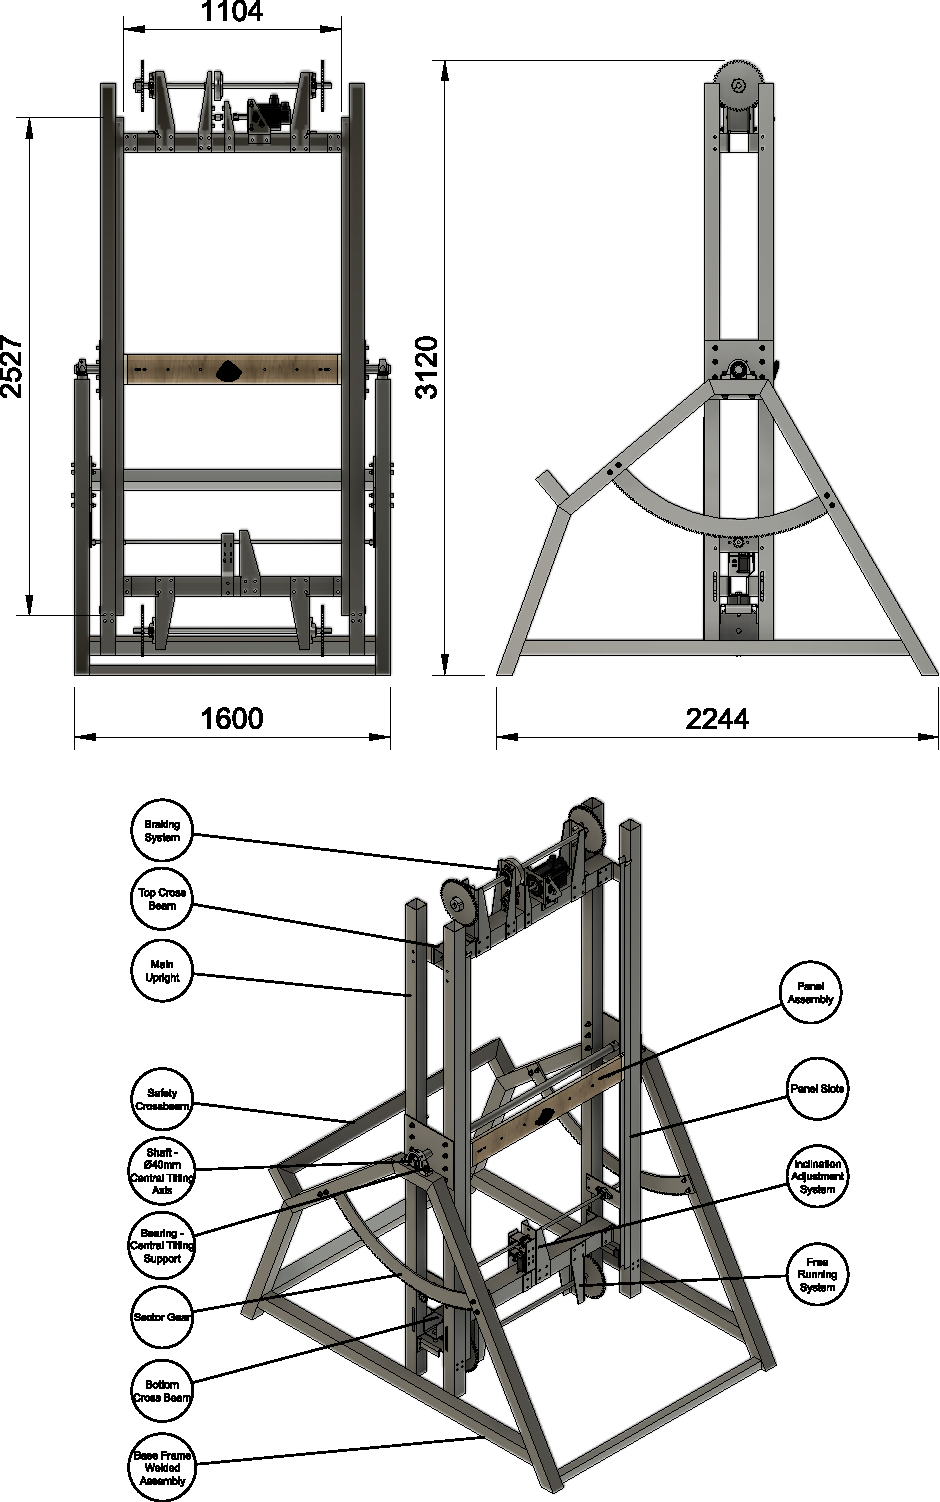
\includegraphics[width=0.9\linewidth]{figs/final_design/Main_Assembly_CAD.pdf}
    \caption{Full Assembly Final CAD Design}
    \label{fig:full-assembly-final-design}
\end{figure}

\begin{figure}[ht]
    \centering
    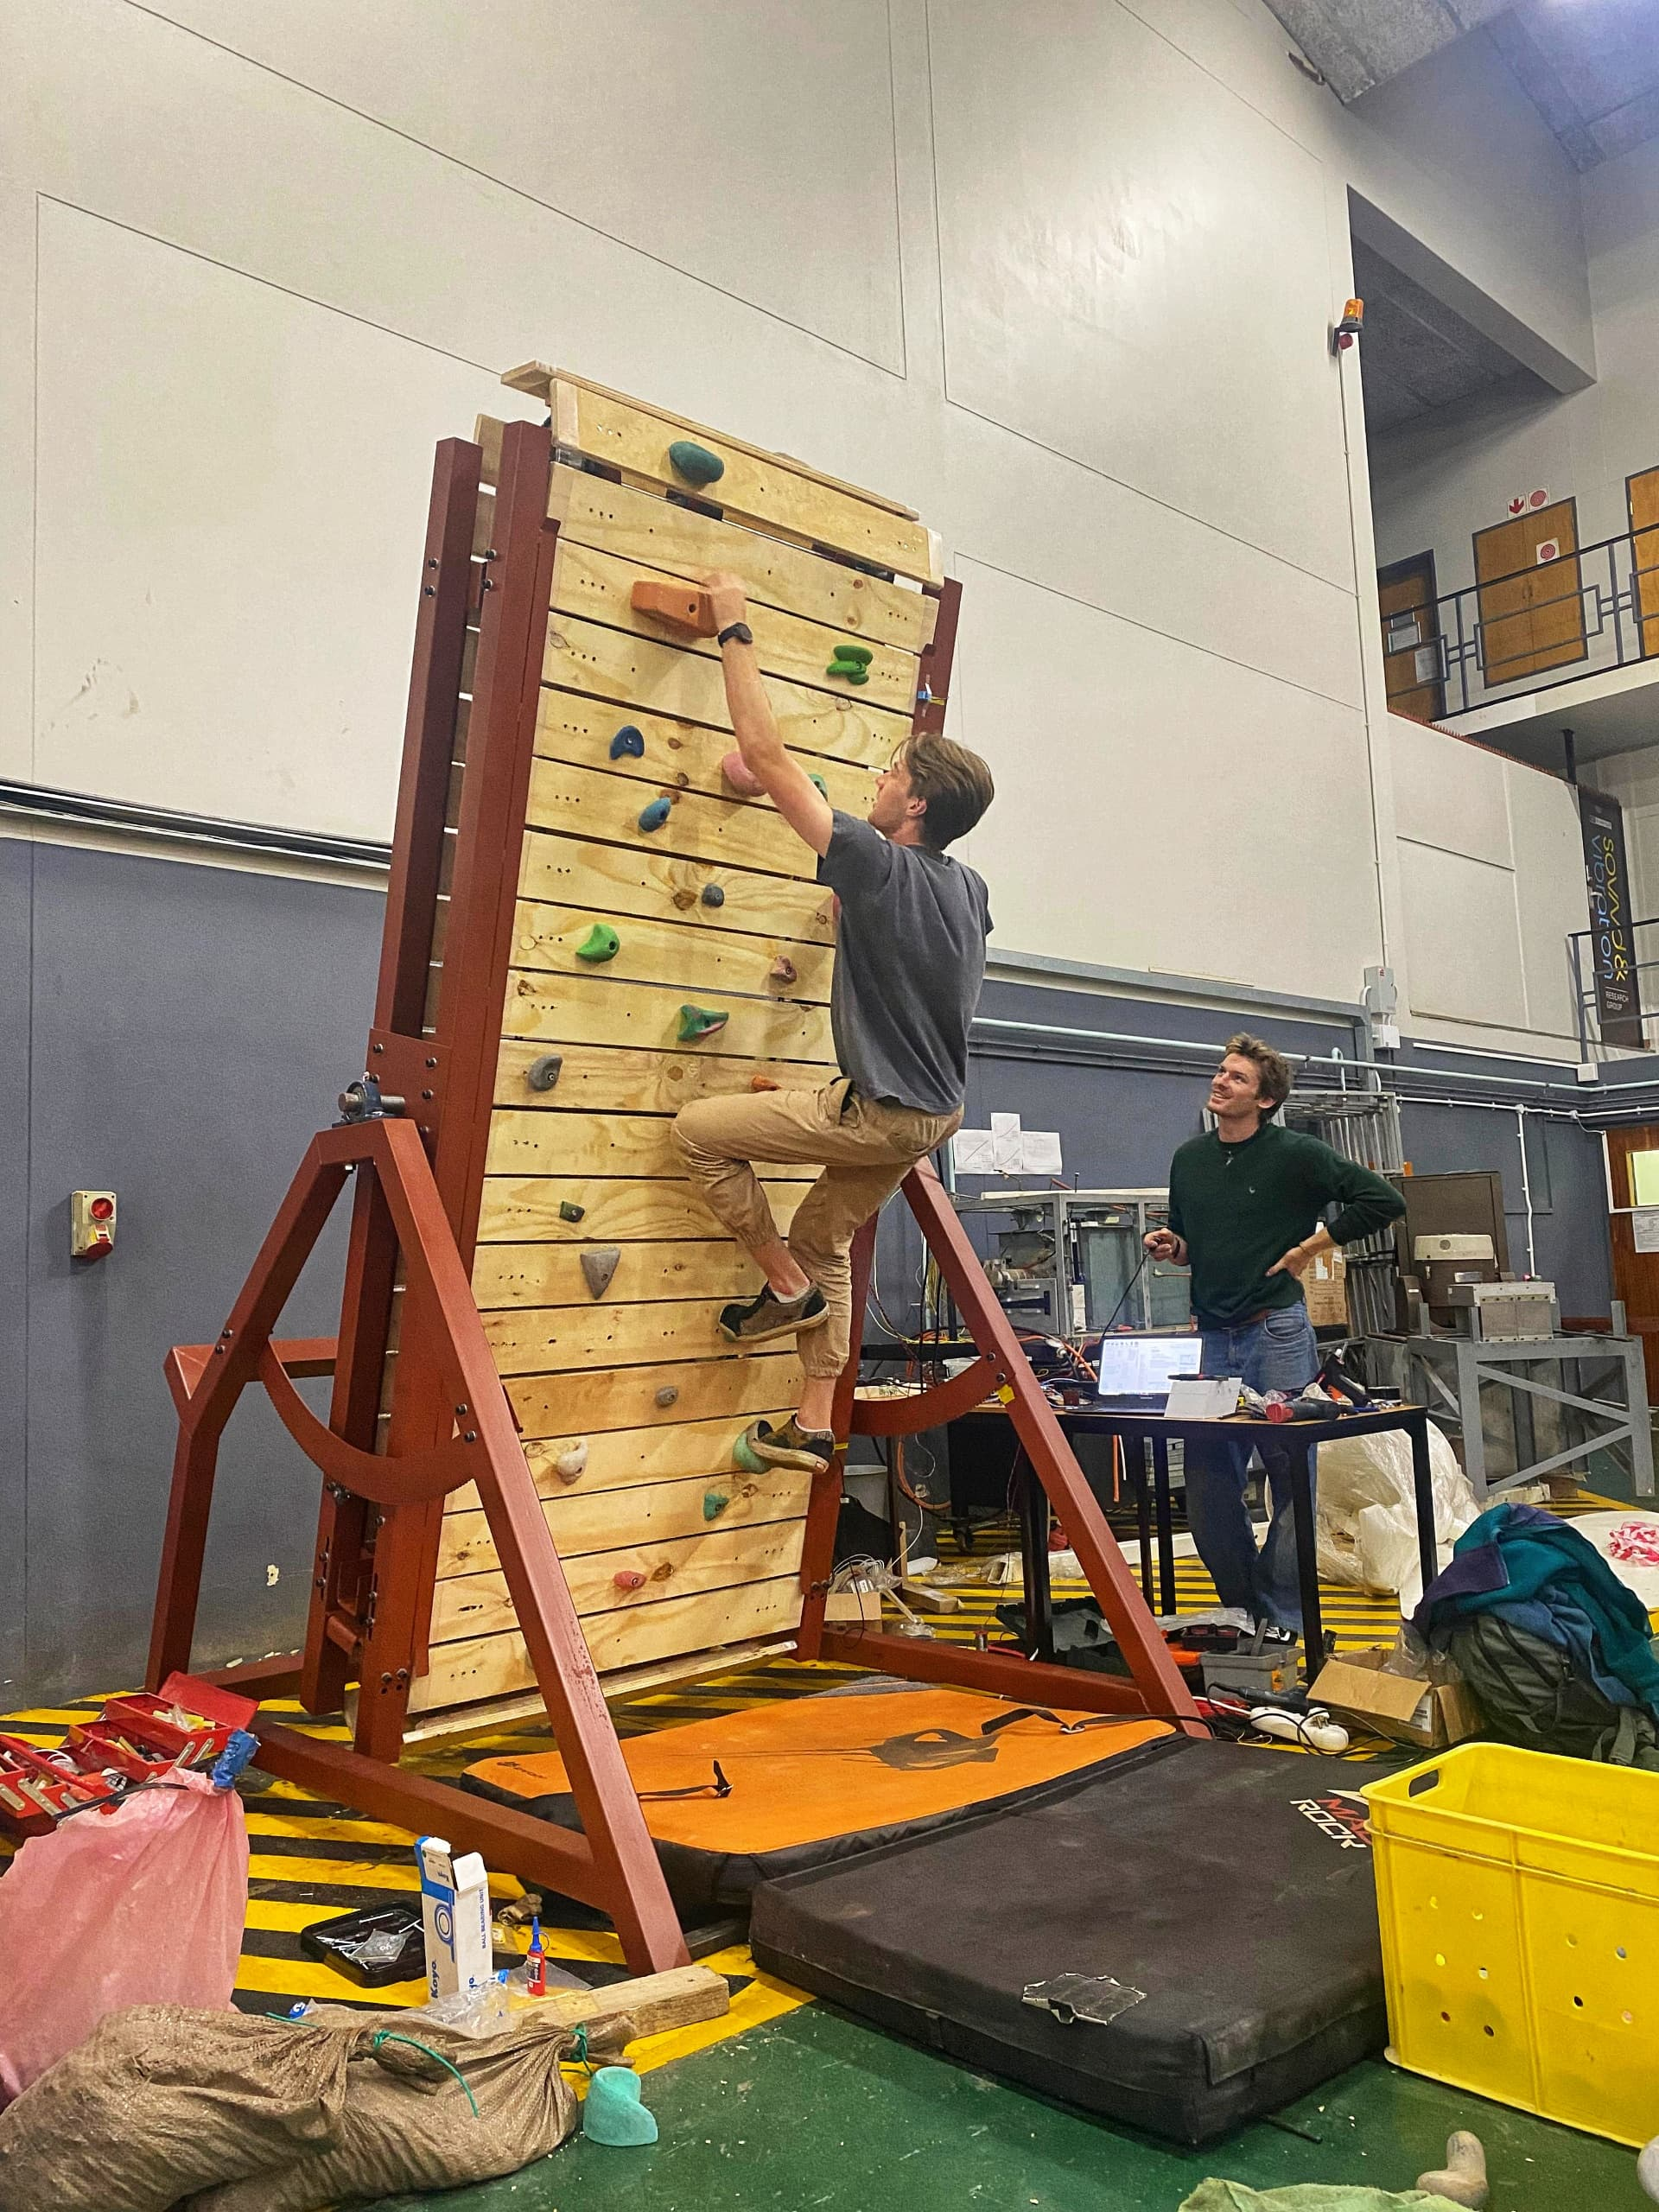
\includegraphics[width=0.9\linewidth]{figs/final_design/zazuwall.jpeg}
    \caption{Completed Rotating Climbing Wall in Use. A video demonstration can be viewed at \url{https://www.youtube.com/shorts/J7KnqL9NdjM}.}
    \label{fig:final-image}
\end{figure}


\section{Electronic Design}

The electronic design of the rotating climbing wall was intentionally kept straightforward to ensure ease of implementation and reliability. The system's electronics are responsible for controlling the inclination adjustment mechanism and providing user feedback through a simple interface.

\subsection{Power Supply and Distribution}

An adjustable DC power supply set to 42\,V powers both the IONI servo motor driver and the NEMA 23 stepper motor driver, simplifying the power infrastructure. A DC-DC buck converter steps down the 42\,V to 12\,V to operate the inductive proximity sensors used as limit switches in the tilting system.

\subsection{Control System}

An Arduino Uno microcontroller serves as the central control unit due to its simplicity and the availability of extensive libraries. The Arduino manages:

\begin{itemize}
    \item Controlling the NEMA 23 stepper motor for precise inclination adjustments.
    \item Reading inputs from inductive proximity sensors acting as limit switches.
    \item Providing a user interface via buttons and an LCD screen.
\end{itemize}


The Arduino pin connections for the control system are summarized in Table \ref{tab:pinout}.

\begin{table}[h!]
\centering
\begin{tabular}{|c|c|c|}
\hline
\textbf{Pin} & \textbf{Function}          & \textbf{Description}                \\
\hline
A0           & Button Input               & Reads analog voltage for buttons    \\
2            & LIMIT\_SENSOR\_MINUS       & Sensor for -46° limit               \\
3            & LIMIT\_SENSOR\_PLUS        & Sensor for +30° limit               \\
4            & LIMIT\_SENSOR\_0           & Sensor for 0° position              \\
5            & \texttt{dirPin}            & Stepper motor direction control     \\
6            & \texttt{stepPin}           & Stepper motor step control          \\
A4 (SDA)     & LCD I2C Data               & I2C data line for LCD               \\
A5 (SCL)     & LCD I2C Clock              & I2C clock line for LCD              \\
\hline
\end{tabular}
\caption{Arduino Pinout Diagram for Rotating Climbing Wall Control System}
\label{tab:pinout}
\end{table}

\subsubsection{Inclination Adjustment and Calibration}

The stepper motor drives the worm gear mechanism to adjust the wall's inclination accurately. Inductive proximity sensors at the limits of motion allow the system to auto-calibrate upon startup, establishing reference points for precise angle positioning. The current inclination angle is displayed on the LCD for user feedback. The Arduino's EEPROM stores the last known position, ensuring retention of calibration after power loss.

\subsection{Braking System Control}

Due to limitations of the available IONI servo motor driver—which could not interface with the Arduino for automated speed control—the braking system was operated manually during testing. Speed setpoints were input via a laptop connected to the driver using testing software. The braking resistor was connected to the driver's designated terminals to safely dissipate regenerative energy during braking.

\subsection{Future Improvements}

To achieve full automation of the wall's rotational speed control, a servo motor driver capable of interfacing with a microcontroller is necessary. This would enable:

\begin{itemize}
    \item Programmatic control of rotation speed based on user input.
    \item Integration of speed adjustments into the existing user interface.
    \item Enhanced safety features, such as automatic shutdown or speed reduction in response to sensor inputs.
\end{itemize}

\subsection{Safety Considerations}

Safety features incorporated into the electronic design include:

\begin{itemize}
    \item Limit switches to prevent the wall from exceeding mechanical limits.
    \item Overcurrent and thermal protection in motor drivers to prevent damage from electrical faults.
    \item A braking resistor to handle regenerative energy safely.
    \item An emergency stop button that cuts power to electronics when pushed.
\end{itemize}

\chapter{Safety, Testing, and Commissioning}
\label{chap:safety_testing_commissioning}

\section{Introduction}
This chapter outlines the safety measures, test protocols, and commissioning procedures to ensure that the rotary climbing wall operates as designed. The testing phase will verify that the mechanical and electrical subsystems meet performance, safety, and durability requirements. For each test, a specific procedure will be followed, and pass/fail criteria will determine the system's readiness for use. All personnel involved in the testing phase will be required to wear the necessary safety gear, including hard boots to protect toes from heavy objects during load testing. Furthermore, two people will always be present during load testing, ensuring that one person can handle the weights while the other observes for potential tips or system failures, ready to intervene if necessary.

\section{Test Protocols}

\subsection{Static Load Testing}
Static load testing verifies the structural integrity of the climbing wall under various loading conditions. Two main tests will be conducted: the static vertical load test and the static inclined load test. 4 20kg rock bags will be used as static weight and will be placed one by one into a bucket attached to an attachment point on the middle of the panels.

\subsubsection{Static Vertical Load Test}
\textbf{Objective:} To ensure that the climbing wall can withstand the maximum expected vertical load without failure.

\textbf{Procedure:}
\begin{enumerate}
    \item Secure the climbing wall in the vertical position.
    \item Apply the maximum designed load (80kg) in the centre of the wooden panels.
    \item Measure deflections and check for any structural deformations.
\end{enumerate}

\textbf{Pass/Fail Criteria:}
\begin{itemize}
    \item \textbf{Pass:} The wall exhibits no permanent deformations. In this test, since the incline angle is 0 degrees, the panels will experience bending in their strongest orientation—along their longitudinal direction. Minimal or no deflection is anticipated because the load is aligned with the structural grain of the panels, which is designed to withstand vertical forces.
    \item \textbf{Fail:} Any visible structural damage or deflections exceeding the calculated safety margin.
\end{itemize}
\noindent
\textbf{Results:} There were no observable failures or deflections in the frame structure or panels after full loading. This test was passed.


\begin{figure}[htbp]
    \centering
    \fbox{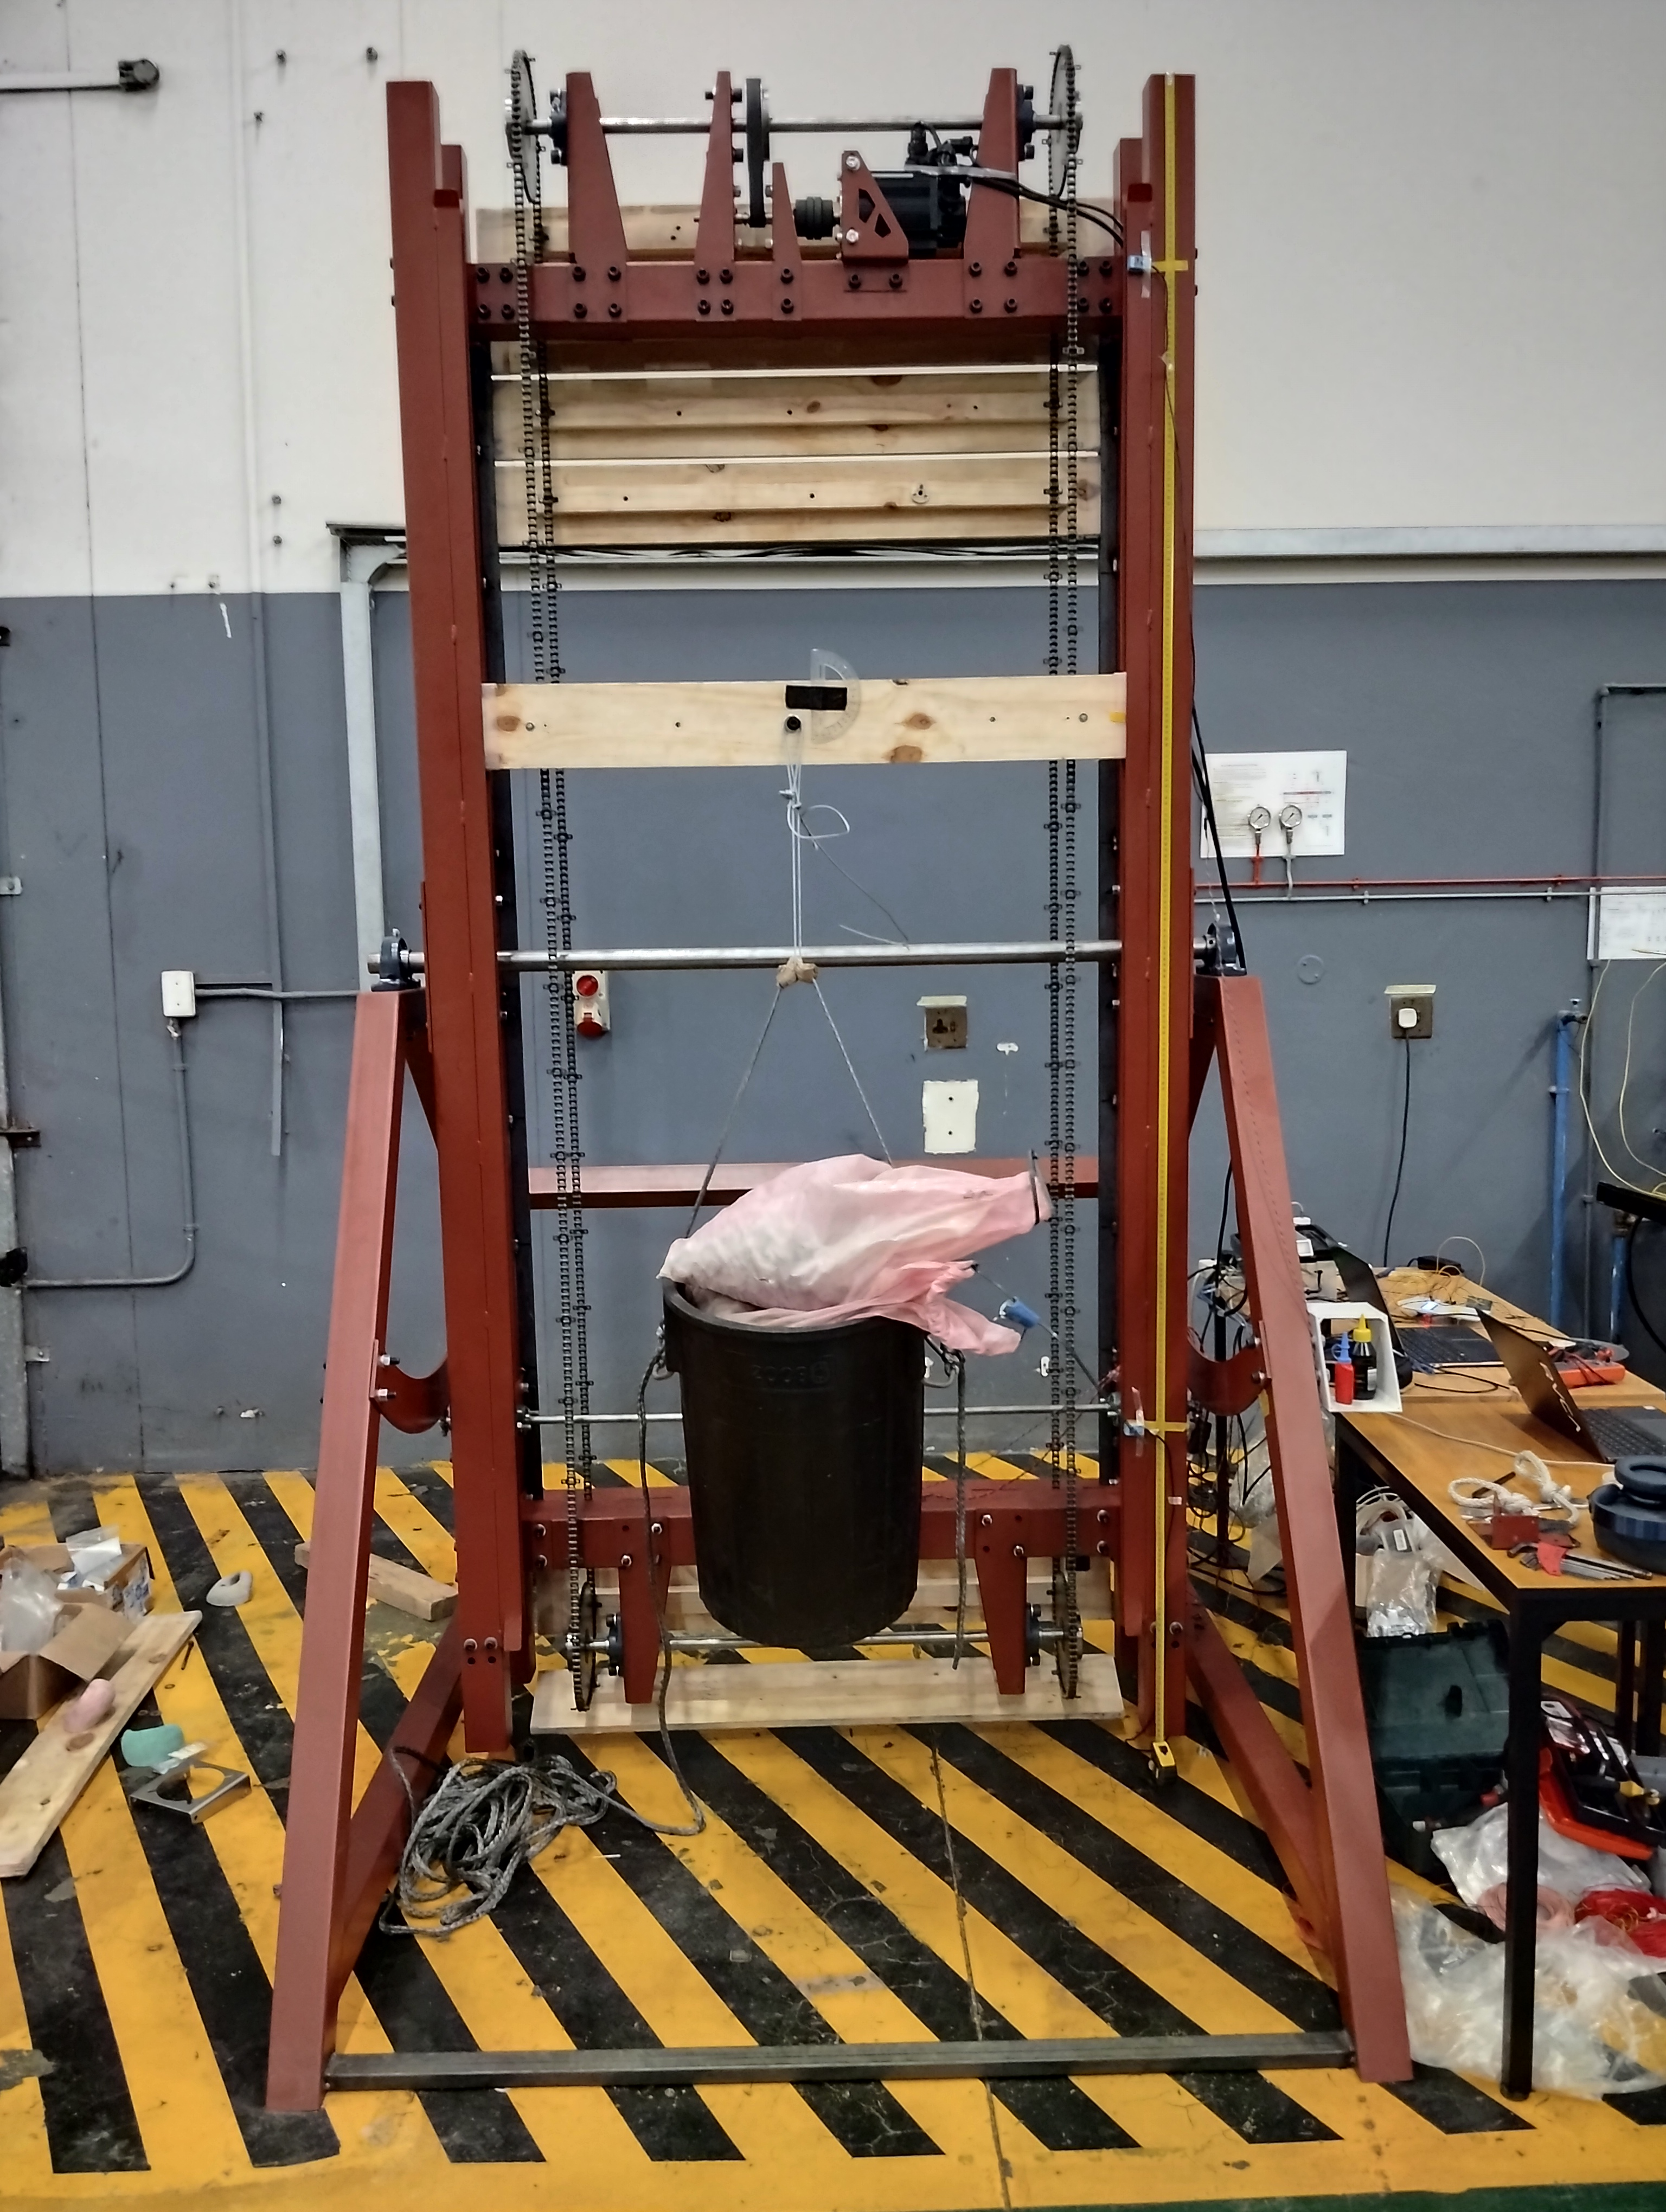
\includegraphics[width=0.8\textwidth]{figs/testing/static_vertical_load_test.jpg}}
    \caption{Static Vertical Load Test}
    \label{fig:static_vertical_load_test}
\end{figure}

\subsubsection{Static Inclined Load Test}
\textbf{Objective:} To verify that the climbing wall can support loads while inclined at various angles.

\textbf{Procedure:}
\begin{enumerate}
    \item Set the climbing wall to its maximum inclined position (45 degrees).
    \item Apply the designed load to simulate a climber at the point of maximum moment arm in order to test for tipping. This point is at the top-most panel with the attachment point in the center of the panel.
    \item Observe the structure for tipping, deflection, and stress concentrations.
\end{enumerate}

\textbf{Pass/Fail Criteria:}
\begin{itemize}
    \item \textbf{Pass:} The wall supports the load without excessive deflection or structural damage.
    \item \textbf{Fail:} Tipping, deformation, or material failure occurs at any point during the test.
\end{itemize}
\noindent
\textbf{Results:}
During the test, an unexpected issue occurred when the shaft holding the worm gear flexed away from the engaged worm wheel, causing a slight slip. This allowed the wall to incline further than intended until it was stopped by the safety beam at the back of the base frame. To proceed with the test, a wooden spacer was placed between the base frame and the tilting frame to remove any force from the worm gear system.\\\\
After the adjustment, the full 80kg load was applied to the center of the panel, resulting in an observed panel deflection of 13.5mm, which was within acceptable limits. The test was repeated after adjusting the worm gear system to ensure better meshing between the gear and worm wheel. In this second attempt, the test was successfully completed with no slippage or failures.


\begin{figure}[htbp]
    \centering
    \fbox{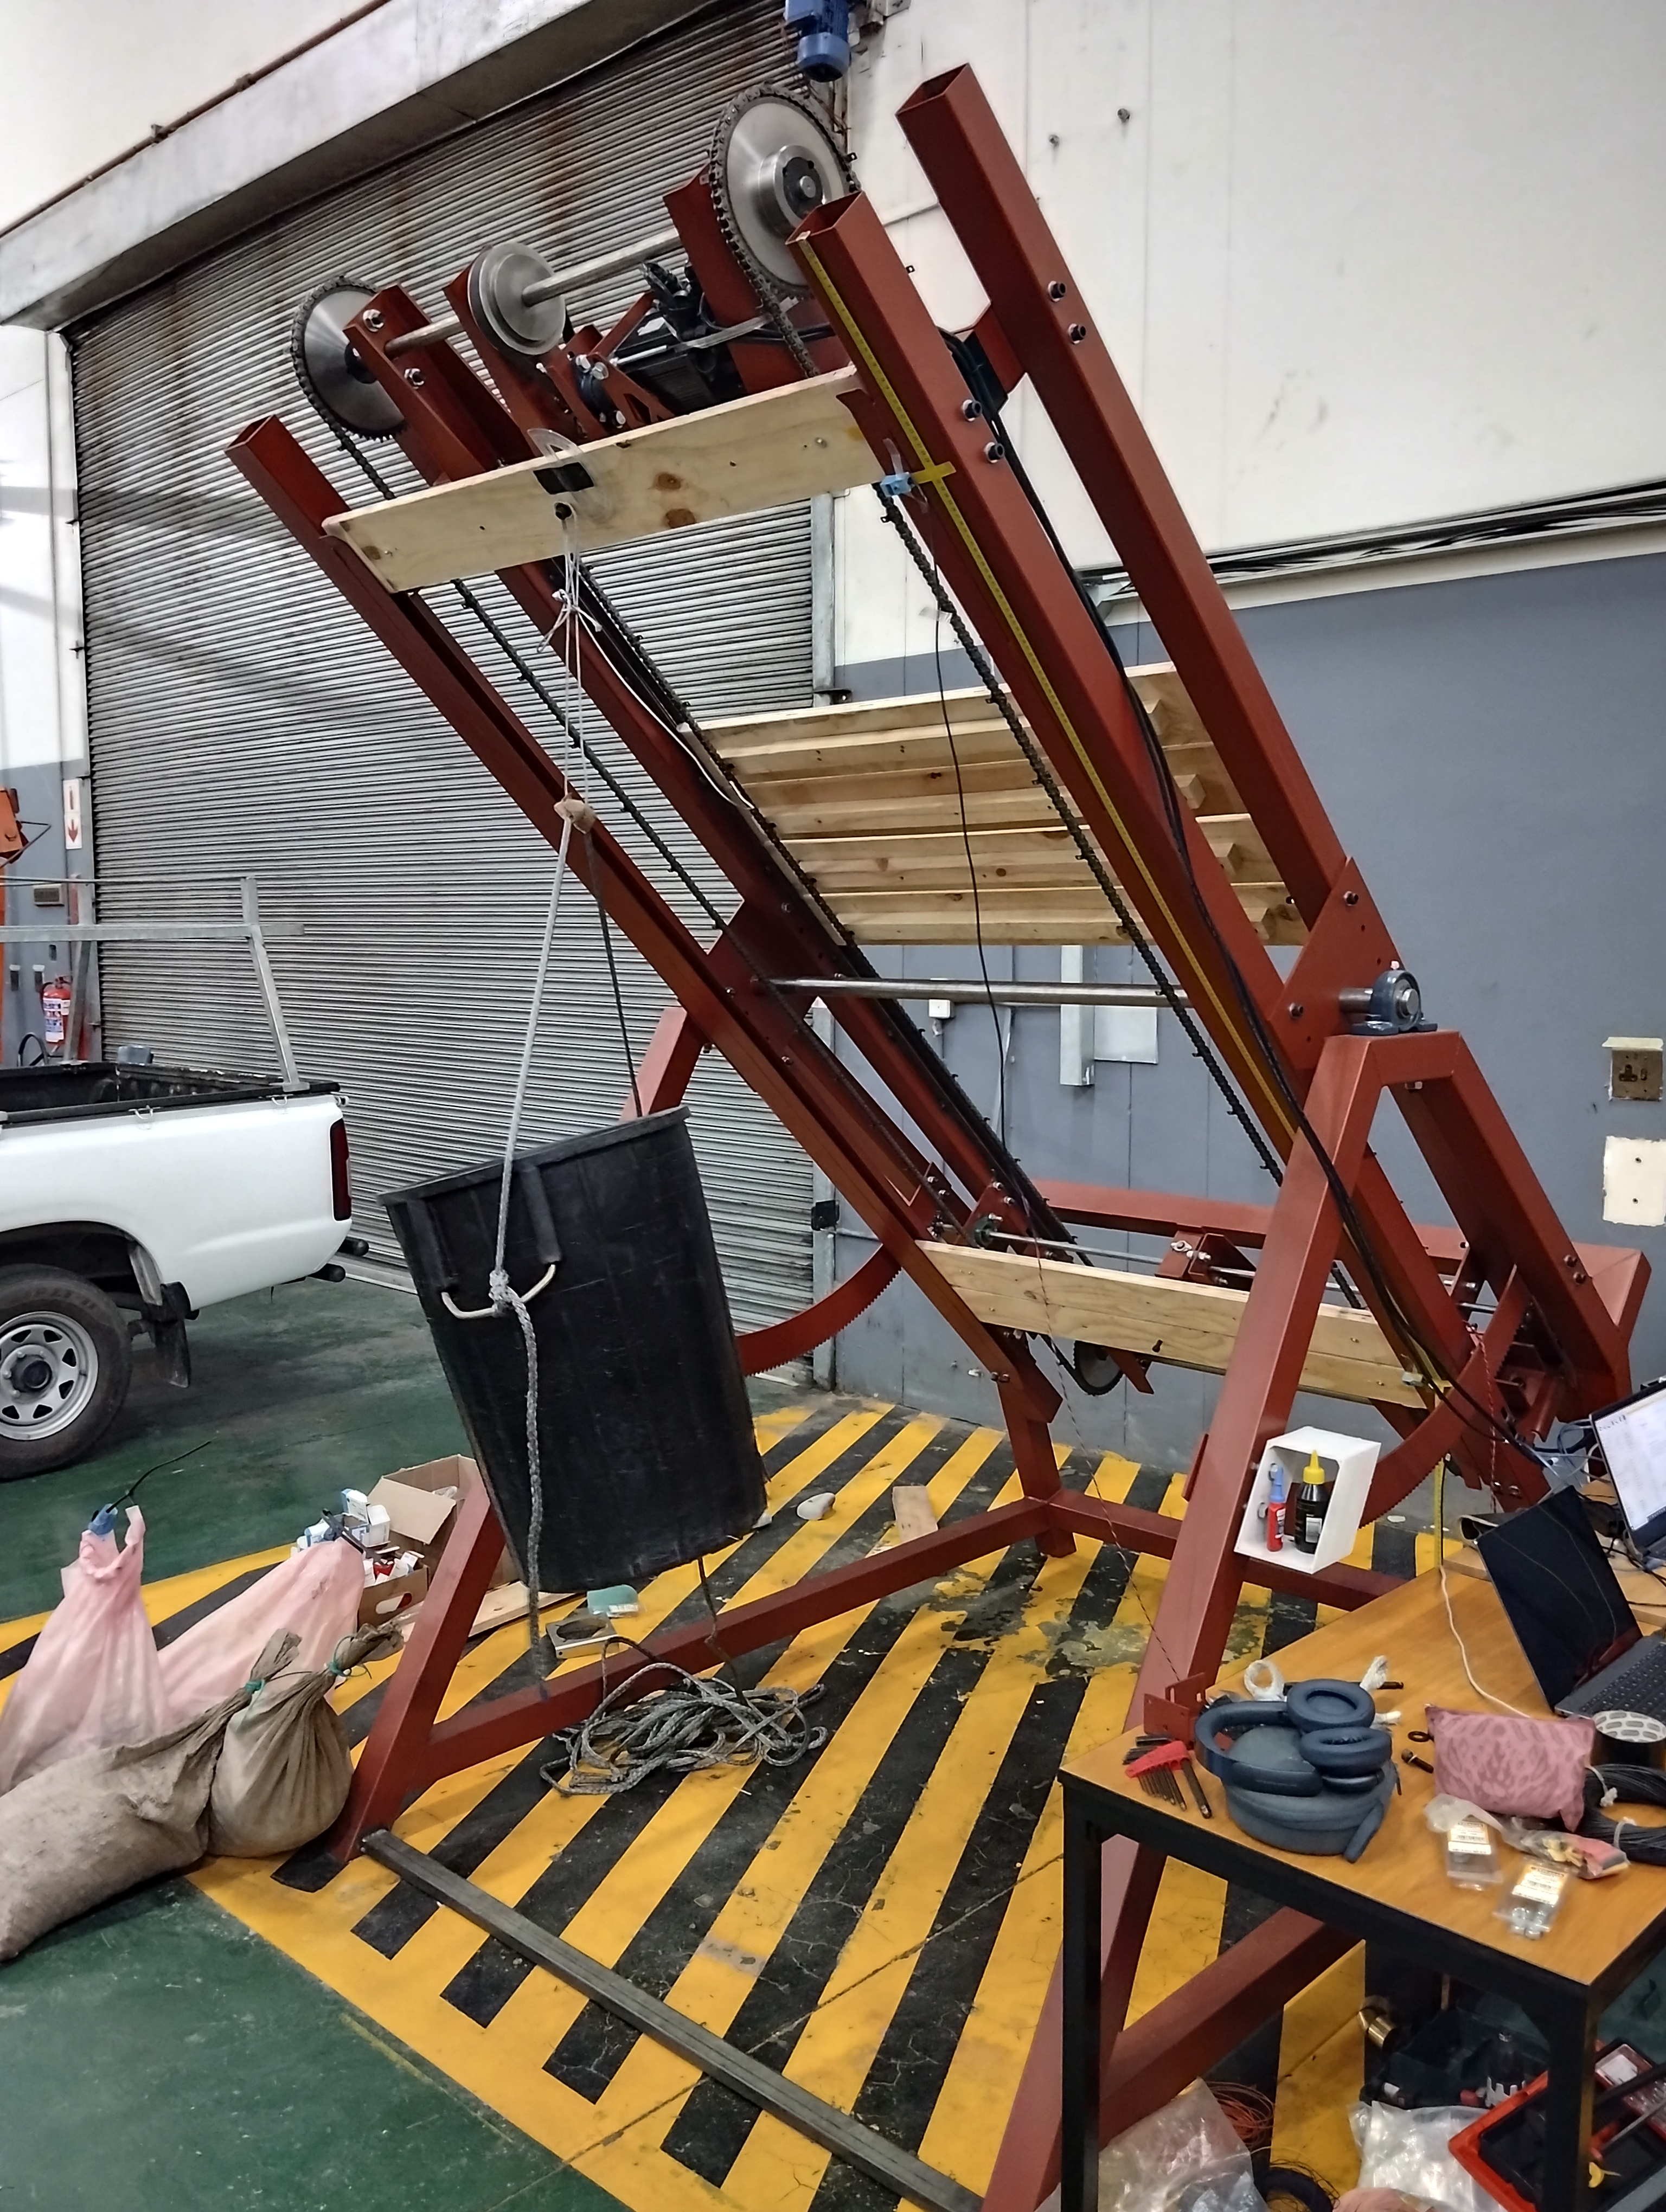
\includegraphics[width=0.8\textwidth]{figs/testing/static_inclined_load_test.jpg}}
    \caption{Static Inclined Load Test}
    \label{fig:static_inclined_load_test}
\end{figure}

\subsection{Operational Testing}
Operational testing ensures that the system functions as intended during dynamic operation, particularly with regard to inclination and speed control.

\subsubsection{Incline Set Test}
\textbf{Objective:} To verify the precision and reliability of the wall's inclination adjustment mechanism.

\textbf{Procedure:}
\begin{enumerate}
    \item Adjust the climbing wall to various preset inclination angles.
    \item Measure the actual angle using a digital angle meter to ensure it matches the setpoint.
    \item Repeat the process multiple times to ensure repeatability.
\end{enumerate}

\textbf{Pass/Fail Criteria:}
\begin{itemize}
    \item \textbf{Pass:} The measured inclination is within ±1° of the setpoint and results are consistent across multiple trials.
    \item \textbf{Fail:} The measured angle deviates significantly from the setpoint or results are inconsistent across trials.
\end{itemize}

\textbf{Results:}
The results of the incline tests are presented in Table \ref{tab:incline_test}. Each test was repeated several times, yielding consistent results.

\begin{table}[H]
\centering
\caption{Incline Set Test Results}
\label{tab:incline_test}
\begin{tabular}{|c|c|c|}
\hline
\textbf{Setpoint (°)} & \textbf{Measured Angle (°)} & \textbf{Error (°)} \\ \hline
+30                  & 30.1                       & +0.1               \\ \hline
+15                  & 15.1                       & +0.1               \\ \hline
0                    & 0.0                        & 0.0                \\ \hline
-10                  & -10.1                      & -0.1               \\ \hline
-20                  & -20.1                      & -0.1               \\ \hline
-45                  & -45.3                      & -0.3               \\ \hline
\end{tabular}
\end{table}

\begin{figure}[H]
    \centering
    \fbox{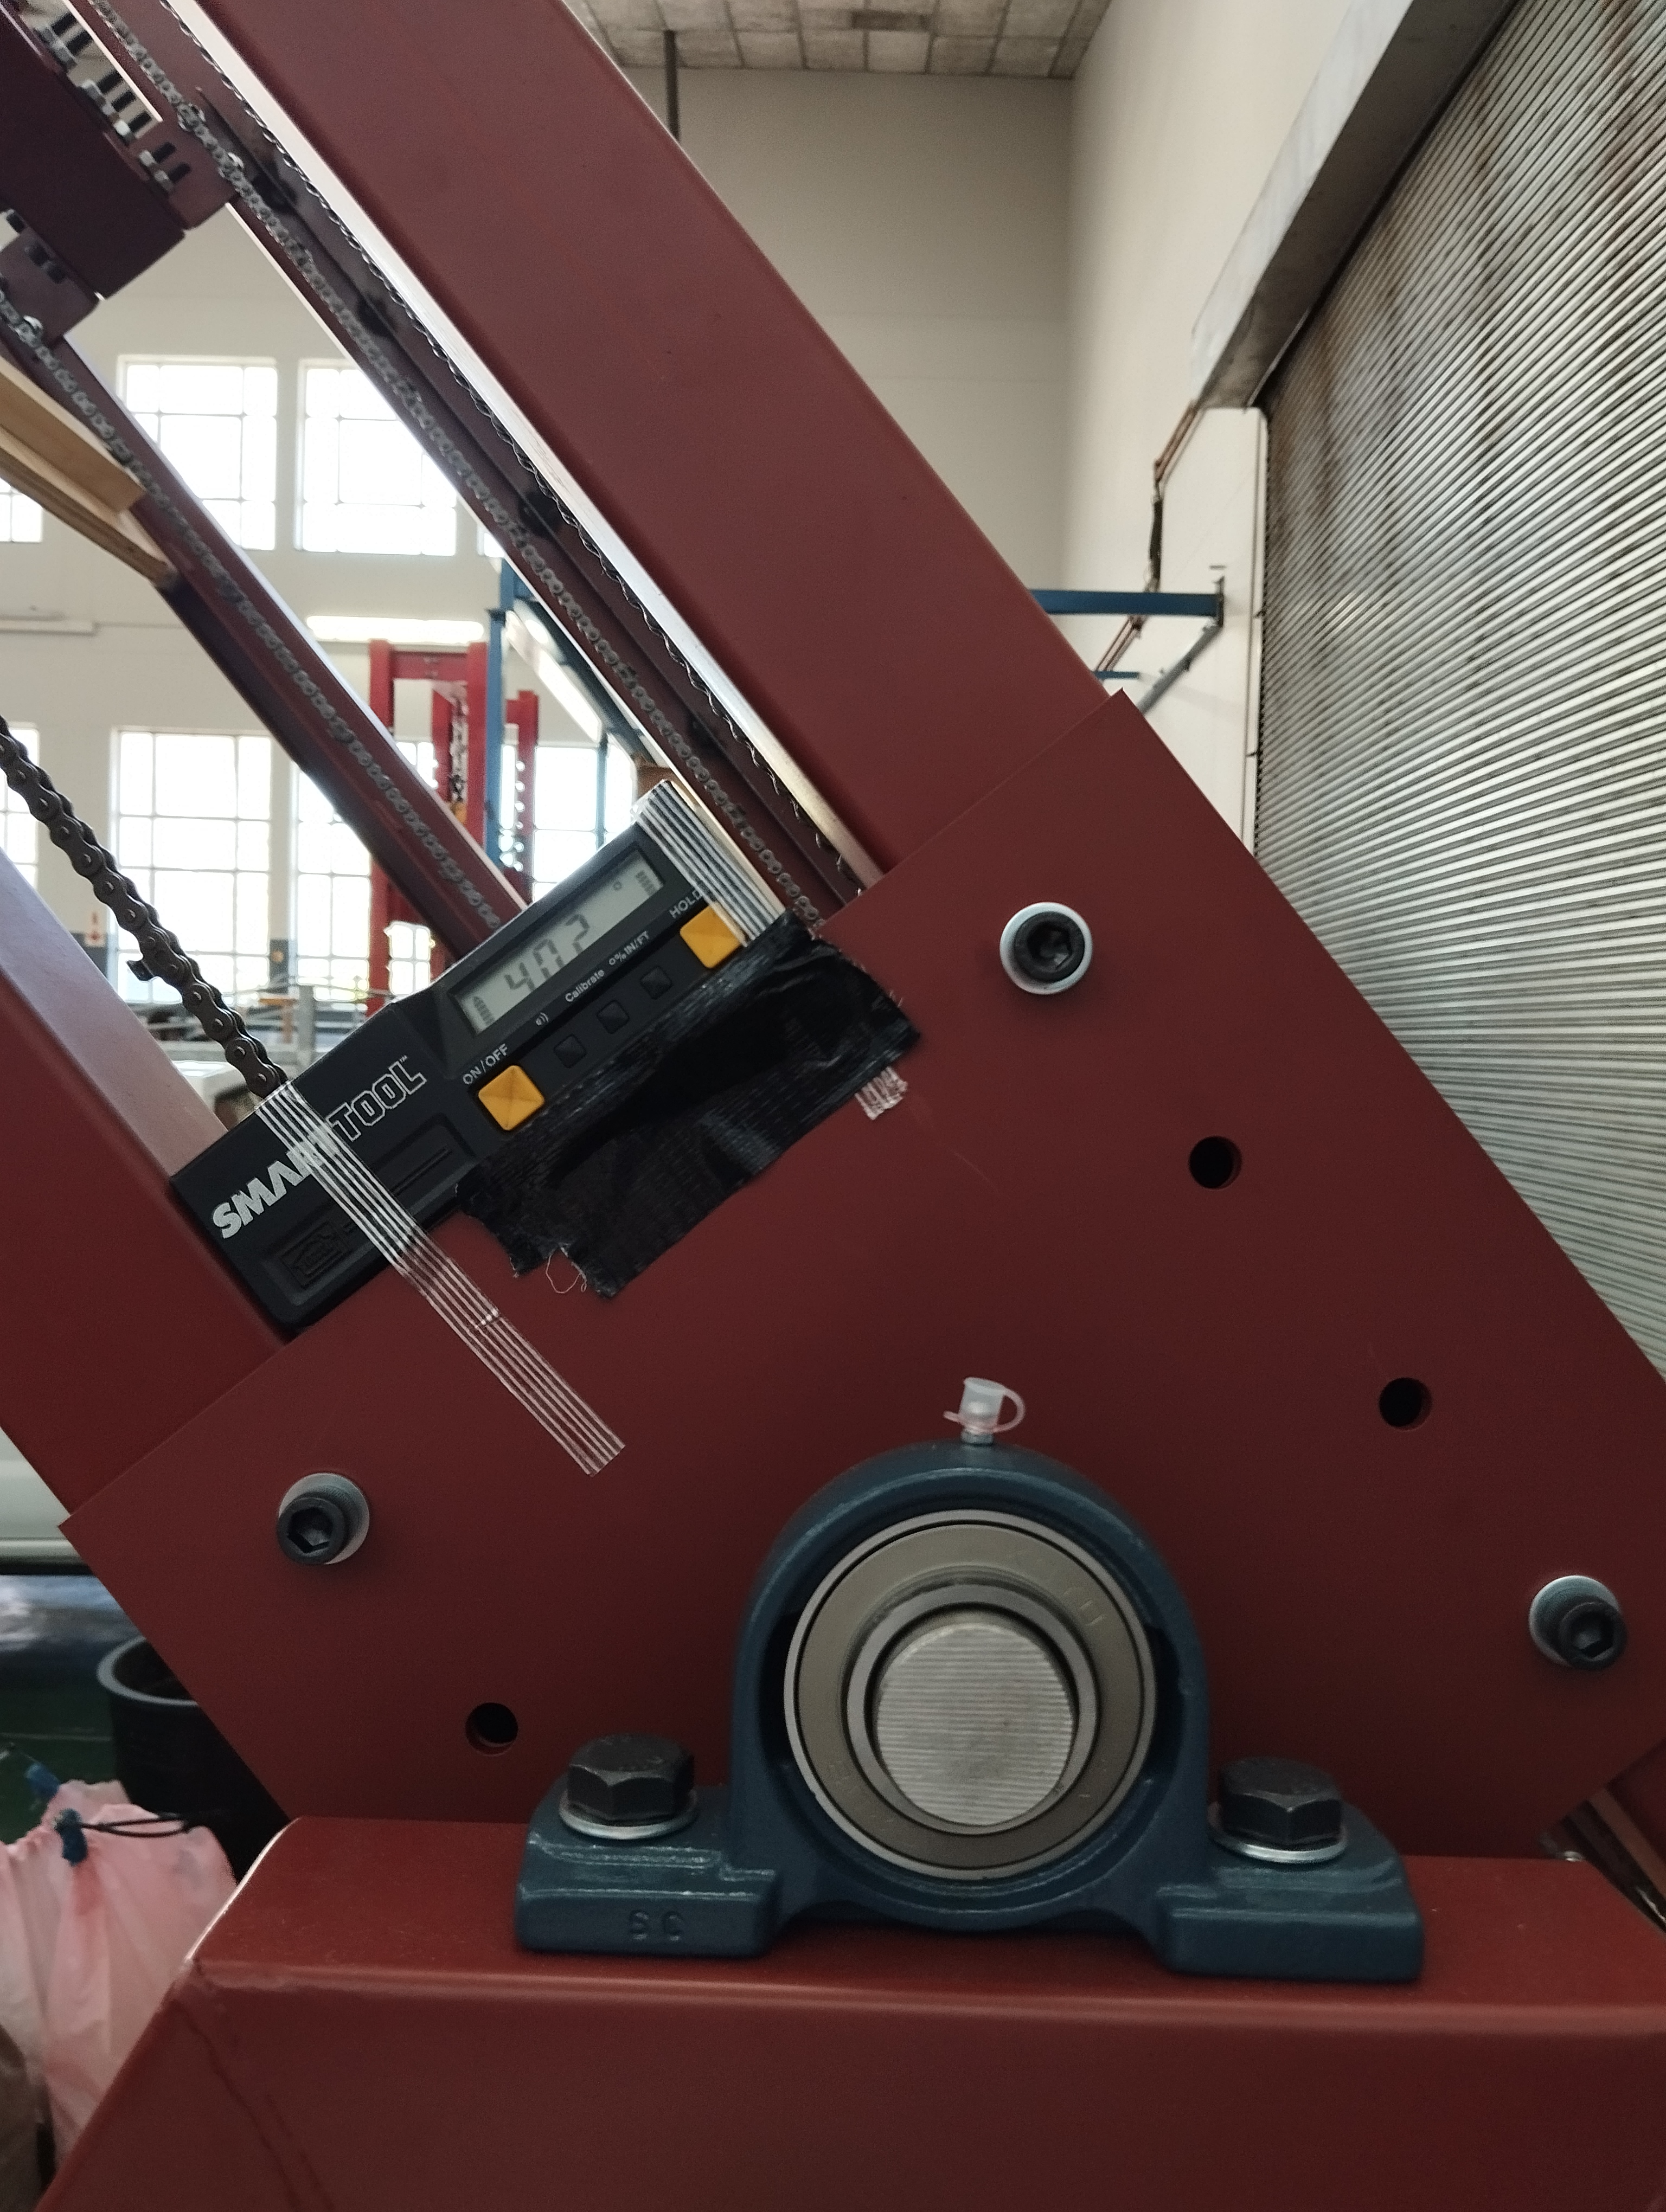
\includegraphics[width=0.8\textwidth]{figs/testing/incline_wall_-40.jpg}}
    \caption{-40 degree Incline Set Test}
    \label{fig:incline_set_test}
\end{figure}

\subsubsection{Speed Test}
\textbf{Objective:} To verify that the climbing wall maintains a consistent speed across different load conditions.

\textbf{Procedure:}
\begin{enumerate}
    \item Set the wall to operate at various speeds (e.g., 15 m/min, 20 m/min, and 25 m/min).
    \item Use two metal proximity sensor switches, along with a metal bracket attached to a panel, to automatically collect speed data.
    \item Measure the time it takes for the panel to pass two points 2 meters apart.
    \item Repeat the process 30 times for each speed.
    \item Calculate the speed for each trial and average the results.
\end{enumerate}

\textbf{Pass/Fail Criteria:}
\begin{itemize}
    \item \textbf{Pass:} The wall operates at the set speed within a tolerance of ±5\%.
    \item \textbf{Fail:} Speed deviations exceed the tolerance, or the system cannot maintain speed under load.
\end{itemize}

\textbf{Results:}
The results of the speed test for 15 m/min, 20 m/min, and 25 m/min are presented in the following tables. Each test was repeated 30 times, and the average speed and standard deviation were calculated for each case.

\begin{table}[H]
\centering
\caption{Speed Test Results for 15 m/min}
\label{tab:speed_test_15}
\begin{tabular}{|c|c|}
\hline
\textbf{Test Number} & \textbf{Speed (m/min)} \\ \hline
1  & 15.00 \\ \hline
2  & 15.00 \\ \hline
3  & 15.00 \\ \hline
4  & 14.90 \\ \hline
5  & 15.09 \\ \hline
...  & ...  \\ \hline
30 & 15.00 \\ \hline
\end{tabular}
\end{table}

The average speed for the 15 m/min setting was \textbf{15.00 m/min}, with a standard deviation of \textbf{0.05 m/min} and a percentage error of \textbf{0\%}.

\begin{table}[H]
\centering
\caption{Speed Test Results for 20 m/min}
\label{tab:speed_test_20}
\begin{tabular}{|c|c|}
\hline
\textbf{Test Number} & \textbf{Speed (m/min)} \\ \hline
1  & 19.99 \\ \hline
2  & 19.99 \\ \hline
3  & 20.00 \\ \hline
4  & 19.99 \\ \hline
5  & 19.99 \\ \hline
...  & ...  \\ \hline
30 & 19.99 \\ \hline
\end{tabular}
\end{table}

The average speed for the 20 m/min setting was \textbf{19.99 m/min}, with a standard deviation of \textbf{0.01 m/min} and a percentage error of \textbf{0.05\%}.

\begin{table}[H]
\centering
\caption{Speed Test Results for 25 m/min}
\label{tab:speed_test_25}
\begin{tabular}{|c|c|}
\hline
\textbf{Test Number} & \textbf{Speed (m/min)} \\ \hline
1  & 23.52 \\ \hline
2  & 24.00 \\ \hline
3  & 23.52 \\ \hline
4  & 23.75 \\ \hline
5  & 23.76 \\ \hline
...  & ...  \\ \hline
30 & 24.00 \\ \hline
\end{tabular}
\end{table}
The average speed for the 25 m/min setting was \textbf{23.74 m/min}, with a standard deviation of \textbf{0.16 m/min} and a percentage error of \textbf{5.04\%}, slightly exceeding the ±5\% tolerance.

\begin{figure}[H]
    \centering
    \fbox{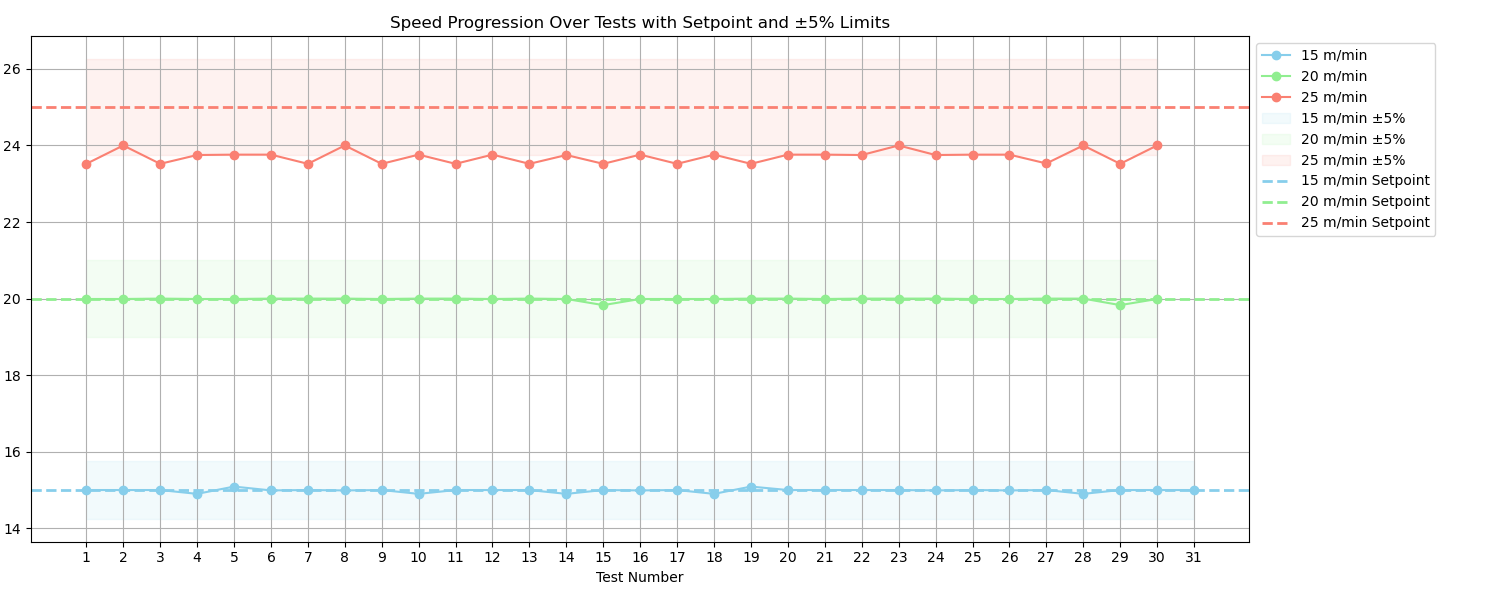
\includegraphics[width=0.8\textwidth]{figs/testing/speed_progression_setpoints_limits.png}}
    \caption{Speed Progression at Various Speeds with Setpoints and ±5\% Limits}
    \label{fig:speed_progression}
\end{figure}

The results show that the climbing wall maintained consistent speeds for the 15 m/min and 20 m/min tests, with deviations well within the ±5\% tolerance. However, the 25 m/min test slightly exceeded the -5\% tolerance below, indicating that adjustments may be needed for higher speeds. It should be noted that this test was performed without the weight of a climber causing the rotation of the wall, so the motor was acting as a motor and not a generator and had to overcome the friction of all the panels in the slots.

\begin{figure}[H]
    \centering
    \fbox{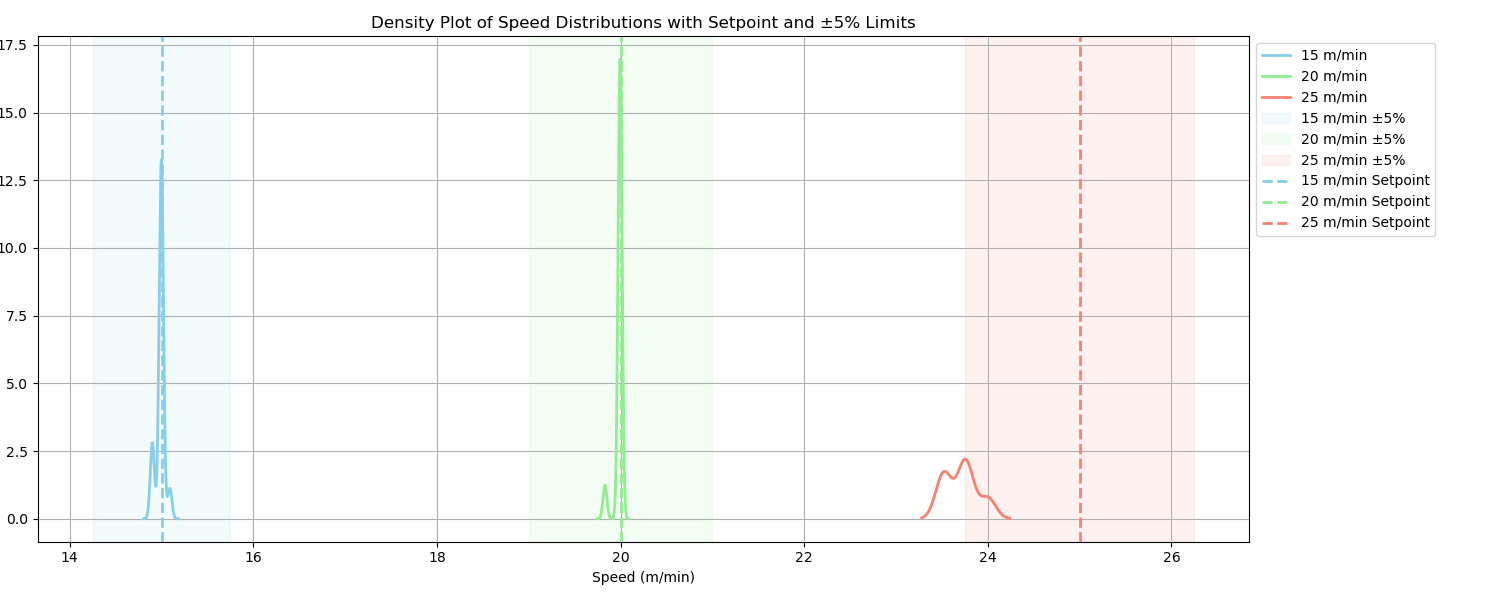
\includegraphics[width=0.8\textwidth]{figs/testing/speed_density_setpoints_limits.png}}
    \caption{Density Plot of Speeds with Setpoints and ±5\% Limits}
    \label{fig:speed_density}
\end{figure}
The density plot shows that the majority of speed measurements for 15 m/min and 20 m/min are centered around their respective setpoints, but exhibit bimodal or even sawtooth-like distributions, as opposed to the expected normal distribution of a perfectly tuned system. This deviation is likely due to over- and undershoot of the speed setpoint caused by oscillations in the system. For the 25 m/min speed, the data was not centered around its setpoint, displaying multiple secondary peaks.

The observed bimodal and multimodal distributions suggest cyclic behavior or oscillations within the control system. Several factors may contribute to this behavior, including:

\begin{itemize}
    \item \textbf{Poorly Tuned PI Controller Gains:} Excessive proportional or integral gains can lead to significant overshoot and undershoot of the speed setpoint, resulting in the cyclical oscillations seen in the data.
    \item \textbf{Mechanical Issues:} Factors such as friction, backlash, or system delays can cause periodic fluctuations around the setpoint, preventing the system from stabilizing at the desired speed.
\end{itemize}

\subsection*{Mitigation Steps}

To address the oscillatory behavior and bring the system closer to the desired performance, the following mitigation steps are recommended:

\begin{itemize}
    \item \textbf{Re-tune the PI Controller:} Adjust the proportional and integral gains to reduce overshoot and improve stability. This could involve reducing the integral gain to prevent windup or fine-tuning the proportional gain to minimize oscillations.
    \item \textbf{Implement Derivative Control:} Adding a derivative term (resulting in a PID controller) may help dampen oscillations and improve the system's ability to reach and maintain the setpoint more consistently.
    \item \textbf{Introduce Damping Mechanisms:} Mechanical damping or filters can reduce the effects of friction or backlash, allowing the system to settle more smoothly around the setpoint.
\end{itemize}

By implementing these mitigation steps, the system should exhibit improved control characteristics, with speed measurements more closely following a normal distribution around the setpoints, and less deviation due to oscillations.




\section{Conclusion}
The testing and commissioning phase is essential to validate the safety and functionality of the rotary climbing wall. All personnel involved in the testing phase adhered to strict safety protocols, including wearing protective gear such as hard boots. During load testing, two people were always present, with one person handling the weights while the other observed for tipping or potential failures. Successful completion of the outlined tests ensures the system meets its design specifications and is ready for operational use.

\chapter{Techno-economic Analysis}
\label{chap:techno_economic_analysis}

This chapter assesses the economic potential of introducing the rotating climbing wall to the South African market, with a brief look at international prospects.

\section{Market Overview}

\subsection{Global and South African Markets}

Rotating climbing walls are a niche within the fitness equipment industry, offering continuous climbing without tall structures. Key global competitors include Treadwall, XClimb Pro, and ClimbStation, which offer models with varying sizes, features, and pricing. In South Africa, the market is largely untapped, with a growing number of climbing gyms but limited access to advanced equipment like rotating walls.

\section{Product Comparison}

The proposed rotating wall features automatic incline and speed adjustments, a customizable control panel, and comprehensive safety features. Its compact design makes it cost-effective to scale, unlike larger and more expensive competitors.

\subsection{Comparison Table}

\begin{table}[H]
\centering
\caption{Comparison of Rotating Climbing Walls}
\label{tab:climbing_wall_comparison_economic}
\resizebox{\textwidth}{!}{%
\begin{tabular}{|p{0.15\linewidth}|c|c|c|c|c|p{0.15\linewidth}|c|c|}
\hline
\textbf{System} & \textbf{Width (m)} & \textbf{Height (m)} & \textbf{Incline Adjustment} & \textbf{Speed Control} & \textbf{Monitoring} & \textbf{Extra Functions} & \textbf{Material} & \textbf{Price (R)} \\
\hline
\textbf{Proposed Product} & 1.1 & 2.53 & Automatic & Automatic & Yes & Advanced Control Panel & Steel/Wood & \textbf{100,000} \\
\hline
XClimb Pro S & 1.5 & 2.82 & No & Yes & No & No & Steel/Wood & 230,000 \\
\hline
XClimb Pro XL & 2.0 & 3.48 & Automatic & Yes & No & No & Steel/Wood & 278,000 \\
\hline
ClimbStation & 1.9 & 3.3 & Automatic & Automatic & Yes & Advanced Control Panel & Aluminium & N/A \\
\hline
Treadwall V4 & 1.22 & 2.97 & No & Manual & Yes & Auto-stop & Steel/Wood & 202,000 \\
\hline
Treadwall Kore4/11 & 1.22 & 2.75 & Manual & Manual & Yes & Auto-stop & Steel/Wood & 140,600 \\
\hline
\end{tabular}
}
\end{table}

\section{Cost and Pricing Strategy}

The prototype costs approximately R52,400, with competitors priced between R140,600 and R278,000. The proposed price is R100,000, which undercuts competitors by nearly 50\%.

\textbf{Production Costs:}
\begin{itemize}
    \item \textbf{Materials}: R52,400
    \item \textbf{Labor}: R15,000
    \item \textbf{Overheads}: R5,000
\end{itemize}

Total production cost is R72,400. With a selling price of R100,000, the profit per unit is R27,600. The breakeven point is 8 units.

\section{Competitive Advantages}

The proposed rotating wall's key advantages are:
\begin{itemize}
    \item Full automation for incline and speed adjustments.
    \item Affordability, making it accessible to a wider market.
    \item Advanced safety features and customization options.
\end{itemize}

\section{Economic Feasibility}

Assuming a target market of 20 potential customers, capturing 50\% of the market within the first year (10 units) is achievable. The profit per unit sold provides a positive return on investment after the breakeven point.

\section{Challenges and Mitigation}

Key challenges include scaling production and creating market awareness. These can be mitigated by partnering with local manufacturers and running targeted marketing campaigns.

\section{Conclusion}

The analysis suggests that the rotating climbing wall is a viable and profitable product in the South African market. Its affordability, automation, and safety features provide a competitive edge, and initial investment can be recovered quickly with minimal sales.

%\chapter{Project Risk Assessment}

This section identifies and outlines potential risks that may negatively impact the project and its ability to be completed.

\begin{itemize}    
    \item \textbf{System Complexity:} The system is quite complex with many moving part that all need to work simultaneously. This creates a risk that if a single part of the system fails or is unable to be completed, the whole system may never work. This can be mitigated via a rigours design and testing process.
    
    \item \textbf{Project Timeline Overrun:} Again, due to the complexity of the project it is possible that the amount of work that needs to be done in order to build a functioning, full-sized prototype will be greater that the time available. If it is clear that this is the case, a scale model could be built as a prototype instead.
    
    \item \textbf{Budget Overrun:} Unexpected costs such as components being more expensive than anticipated, or duplicates of components needing to be bought to replace faulty is a possible risk. Mitigation may include applying for additional budget or self-funding the overshoot.
    
    \item \textbf{User Safety:} Due to the system being quite large with motor that has the potential to provide enough torque to lift a fully grown human. There is risk that the system may perform erratically, injuring the people around it. A safety system and a power cutoff switch must be implemented into the design.
    

\end{itemize}




\chapter{Conclusions}

The sport of rock climbing is growing quickly, and with the increase in professional athletes and competitions (especially the Olympic Games), there is a greater demand for more effective ways to train. This project looks at the feasibility of developing a rotating climbing wall that can be used by rock climbers wanting to train harder and  longer routes with limited vertical space. Investigation into current designs will take place, leading to the development of a final design and manufacture of a functional prototype. \\\\
All the expertise required to successfully complete this project is available to the team involved. The expected total costs are R330,600 over the 8 month expected period. Risks that may hinder the project's ability to be completed are outlined below and mitigation measures have been discussed.

% Start the appendices
\appendix % Switch to appendix mode

% Change chapter numbering style to letters
\renewcommand{\thechapter}{\Alph{chapter}}

% Redefine \chaptertitlename to "Appendix"
\renewcommand{\chaptertitlename}{Appendix}

% Ensure section numbering is \thechapter.\arabic{section}
\renewcommand{\thesection}{\thechapter.\arabic{section}}

% Redefine \titleformat for chapters in the appendix
\titleformat{\chapter}[display]
{\normalfont\huge\bfseries}{\chaptertitlename\ \thechapter}{20pt}{\Huge}
\titlespacing*{\chapter}{0pt}{-50pt}{20pt}
\titlespacing*{\section}{0pt}{15pt}{10pt}

% Adjust figure and table numbering if necessary
\numberwithin{figure}{chapter}
\numberwithin{table}{chapter}
\renewcommand{\thefigure}{\thechapter.\arabic{figure}}
\renewcommand{\thetable}{\thechapter.\arabic{table}}

% Include each appendix as separate chapters
\chapter{FEM Verification}
\label{appx:FEM-verification}

This appendix provides the detailed process of verifying the structural analysis of the rotating climbing wall using both analytical calculations and Fusion 360 simulations for a cantilever beam setup.

\section{Introduction}
To ensure the structural integrity of the rotating climbing wall, a verification process was conducted by comparing the results from Fusion 360's static simulation with analytical calculations for a cantilever beam setup.

\section{Test Case Setup}
\subsection{Geometry}
A 76\,mm $\times$ 76\,mm $\times$ 2\,mm mild steel square tube, with a length of 2\,m, was used as the cantilever beam geometry for this verification.

\subsection{Material Properties}
The material properties applied for both the analytical calculations and the Fusion 360 simulations were as follows:
\begin{itemize}
    \item \textbf{Material:} Steel
    \item \textbf{Density:} $7.850 \times 10^{-6}$\,kg/mm\textsuperscript{3}
    \item \textbf{Young's Modulus:} 210\,GPa
    \item \textbf{Poisson's Ratio:} 0.30
    \item \textbf{Yield Strength:} 207\,MPa
    \item \textbf{Ultimate Tensile Strength:} 345\,MPa
\end{itemize}

\subsection{Boundary Conditions and Loading}
The cantilever beam was analyzed under the following conditions:
\begin{itemize}
    \item One end of the beam was fully fixed.
    \item A point load of 1000\,N was applied at the free end of the beam.
\end{itemize}

\section{Analytical Calculations}
The maximum bending stress and maximum deflection of the cantilever beam are calculated using the following formulas:

\begin{itemize}
    \item \textbf{Maximum Bending Stress:}
    \[
    \sigma_{\text{max}} = \frac{M \cdot c}{I} = \frac{P \cdot L \cdot c}{I} = \frac{1000\,\text{N} \times 2\,\text{m} \times 0.038\,\text{m}}{7.14 \times 10^{-6}\,\text{m}^4} = 140.56\,\text{MPa}
    \]
    \item \textbf{Maximum Deflection:}
    \[
    \delta_{\text{max}} = \frac{P \cdot L^3}{3 E I} = \frac{1000\,\text{N} \times 2^3\,\text{m}^3}{3 \times 210 \times 10^9\,\text{Pa} \times 7.14 \times 10^{-6}\,\text{m}^4} = 23.49\,\text{mm}
    \]
\end{itemize}

Where:

\begin{itemize}
    \item \( P = 1000\,\text{N} \) (applied load)
    \item \( L = 2\,\text{m} \) (length of the beam)
    \item \( c = \dfrac{76\,\text{mm}}{2} = 38\,\text{mm} = 0.038\,\text{m} \) (distance from the neutral axis to the outer fiber)
    \item \( I = \dfrac{(76\,\text{mm})^4 - (72\,\text{mm})^4}{12} = 7.14 \times 10^{-6}\,\text{m}^4 \) (second moment of area)
    \item \( E = 210 \times 10^9\,\text{Pa} \) (Young's modulus)
\end{itemize}

\section{Fusion 360 Simulation Setup}
The same material properties, boundary conditions, and load were applied in the Fusion 360 simulation as depicted in figures \ref{fig:max_stress} and \ref{fig:max_deflection}. A mesh sensitivity analysis was performed to ensure accurate capture of stress concentrations, particularly near the fixed end and the point load application.

\section{Results Comparison}
The results from the analytical calculations and Fusion 360 simulation were compared for maximum bending stress and deflection:

\begin{table}[H]
    \centering
    \begin{tabular}{|>{\centering\arraybackslash}p{0.35\linewidth}|>{\centering\arraybackslash}p{0.2\linewidth}|>{\centering\arraybackslash}p{0.2\linewidth}|>{\centering\arraybackslash}p{0.15\linewidth}|}
        \hline
        \textbf{Parameter} & \textbf{Analytical Result} & \textbf{Fusion 360 Result} & \textbf{Percentage Error (\%)} \\
        \hline
        Maximum Bending Stress (MPa) & 140.56 & 148.34 & 5.53 \\
        \hline
        Maximum Deflection (mm) & 23.49 & 23.62 & 0.57 \\
        \hline
    \end{tabular}
    \caption{Comparison of Analytical and Fusion 360 Simulation Results for Cantilever Beam}
    \label{tab:comparison_results}
\end{table}

\section{Conclusion}
The comparison demonstrates that the Fusion 360 simulation results align closely with the analytical calculations, with small percentage errors. This suggests that the simulation results are reliable for this application. Further refinement of simulation parameters, such as mesh density, could further improve the accuracy.

\begin{figure}[H]
    \centering
    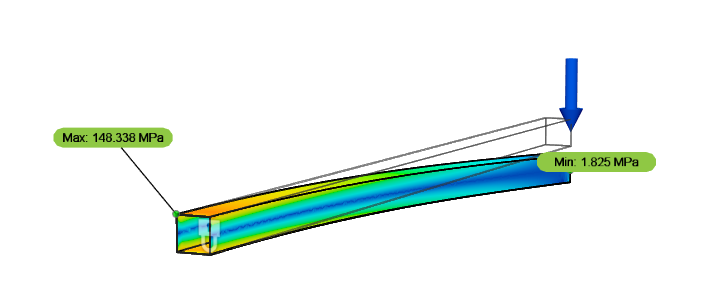
\includegraphics[width=1\textwidth]{figs/FEM/cantilever_beam_stress.png} 
    \caption{Fusion 360 Simulation Result: Maximum Bending Stress for Cantilever Beam}
    \label{fig:max_stress}
\end{figure}

\begin{figure}[H]
    \centering
    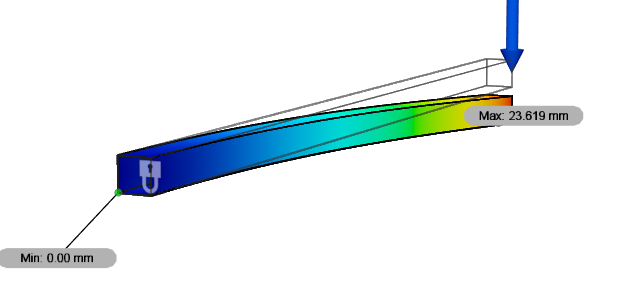
\includegraphics[width=1\textwidth]{figs/FEM/cantilever_beam_disp.png} 
    \caption{Fusion 360 Simulation Result: Maximum Deflection for Cantilever Beam}
    \label{fig:max_deflection}
\end{figure}

\include{chaps-append/chap-Calculations}
\chapter{Techno-Economic Analysis}

\section{Budget}
\label{appx:skripsie-budget}

\begin{table}[ht]
    \centering
    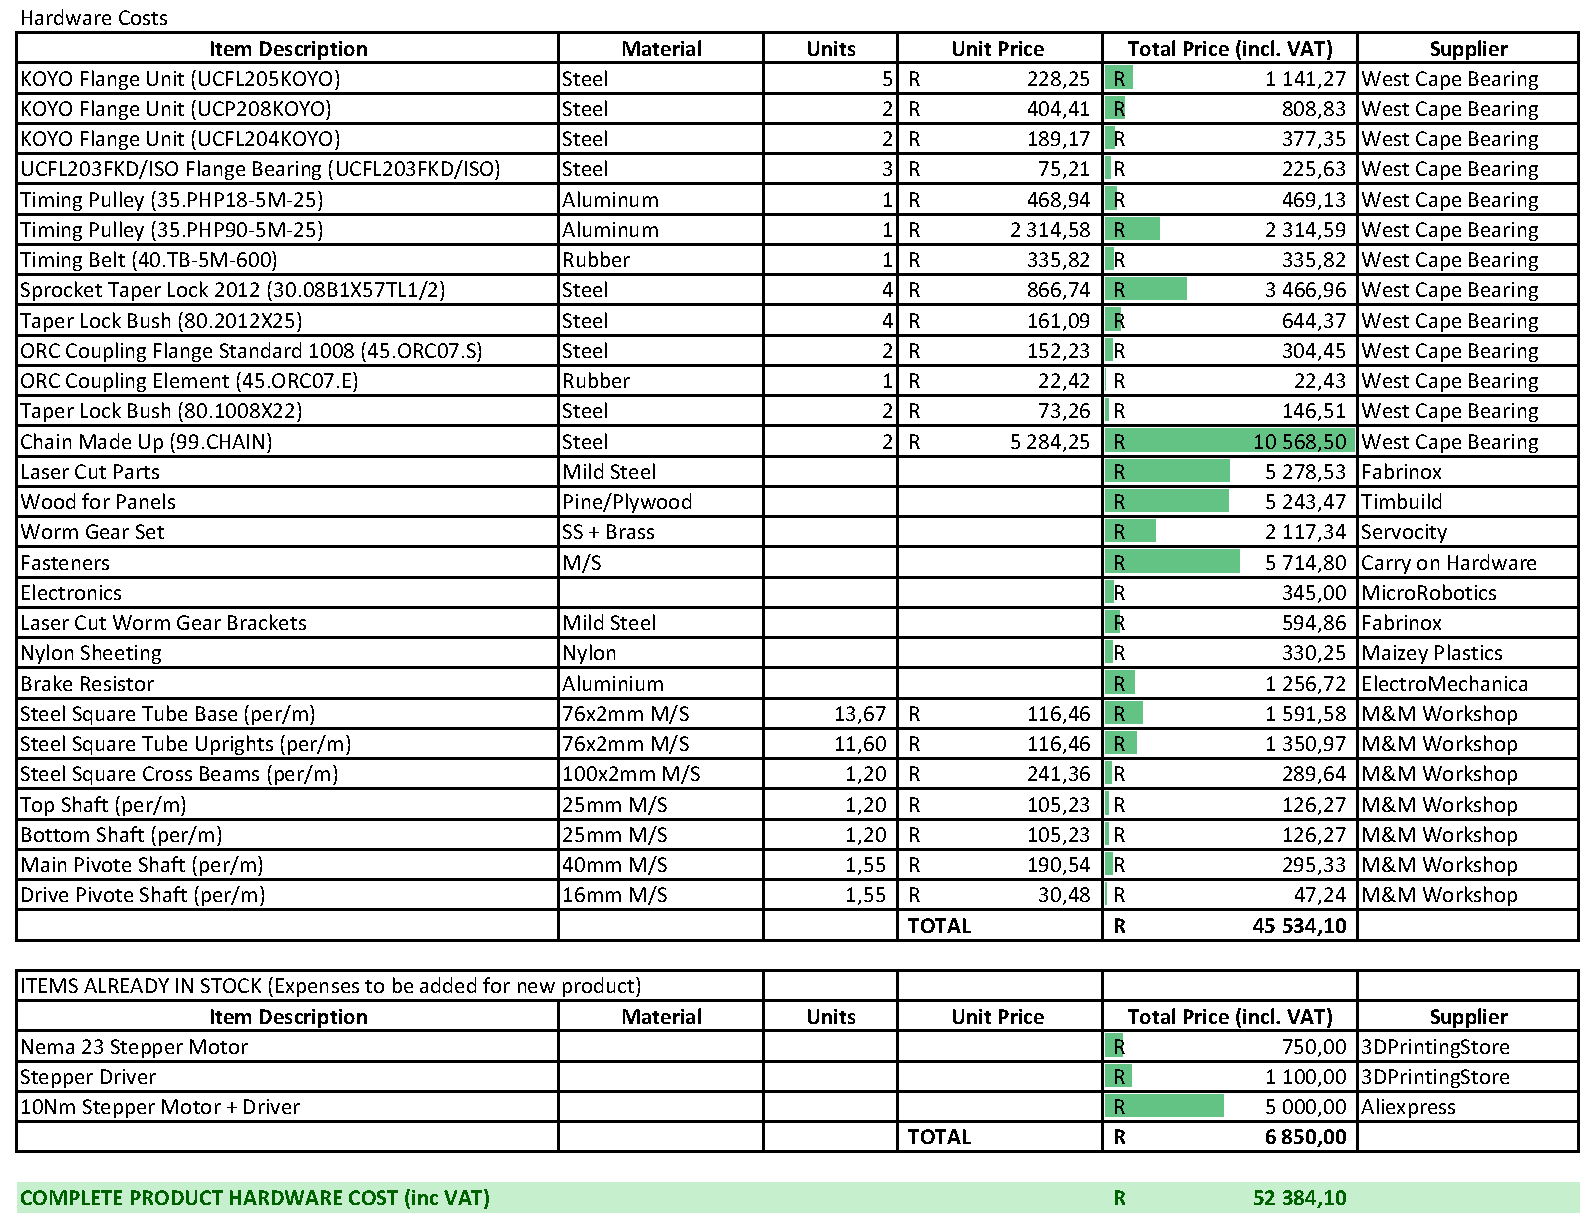
\includegraphics[width=1\linewidth]{tables/hardware_BOM.pdf}
    \caption{Hardware Bill of Materials}
    \label{tab:hardware-BOM}
\end{table}


\begin{table}[ht]
    \centering
    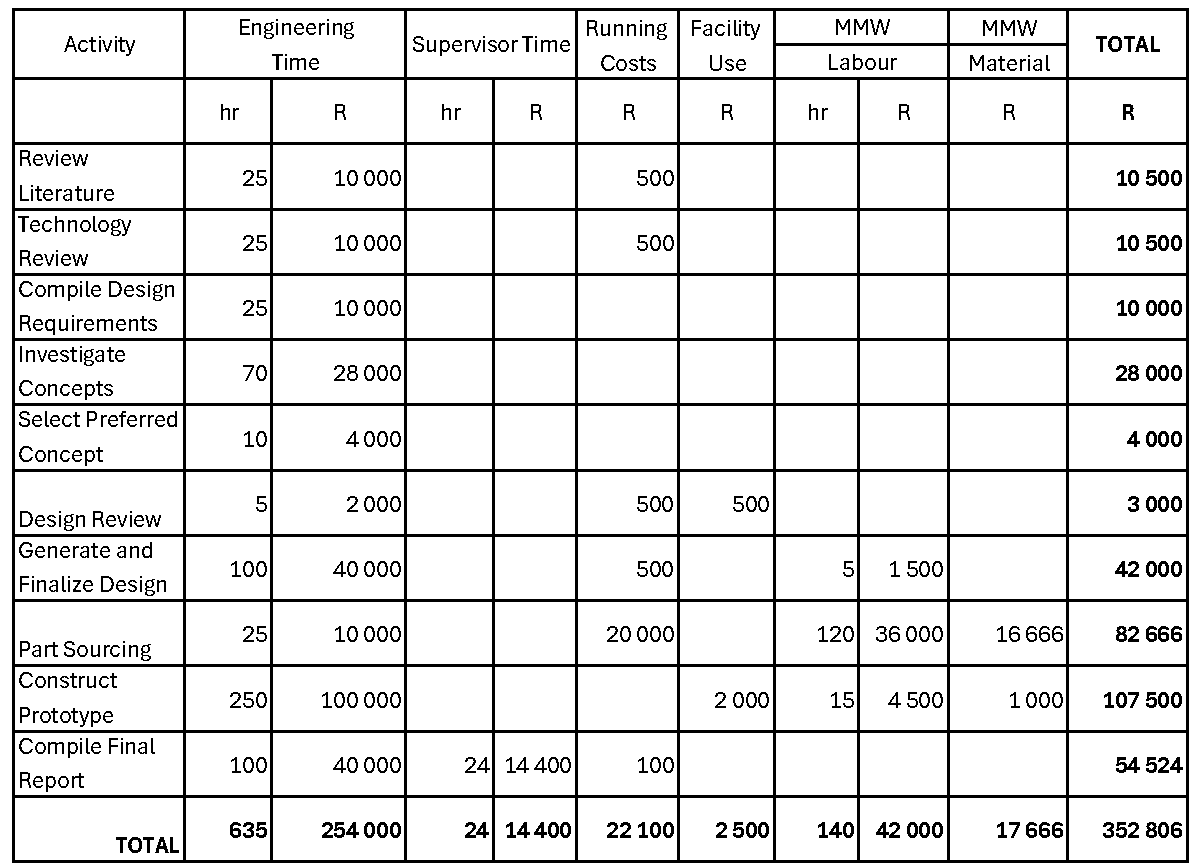
\includegraphics[width=1\linewidth]{tables/skripsie_budget_1.pdf}
    \caption{Proposed Skripsie Budget}
\end{table}

\begin{table}[ht]
    \centering
    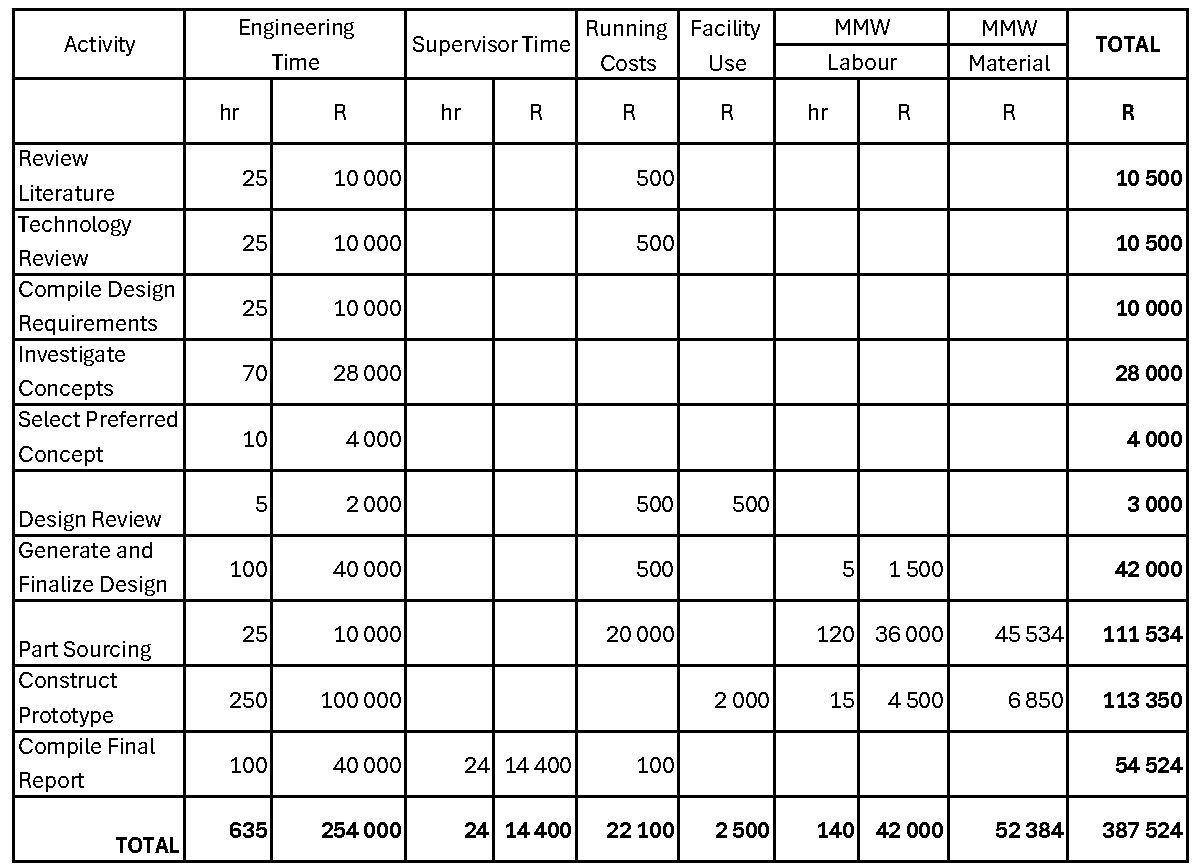
\includegraphics[width=1\linewidth]{tables/skripsie_budget_2.pdf}
    \caption{Realized Skripsie Budget}
\end{table}

\section{Time Management}

The project was completed on time, largely due to significant progress made during the June/July recess, focusing on research and finalizing the CAD design. This allowed the final drawing pack to be submitted to the workshop in the first week of the second semester, enabling fabrication to begin promptly. Some minor delays occurred during the manufacturing phase, mainly due to material sourcing and small design adjustments, which caused a slight postponement in the construction timeline. The Gantt chart depicting the project's progress is shown in Figure \ref{fig:gantt_final}.

\begin{figure}[ht]
    \centering
    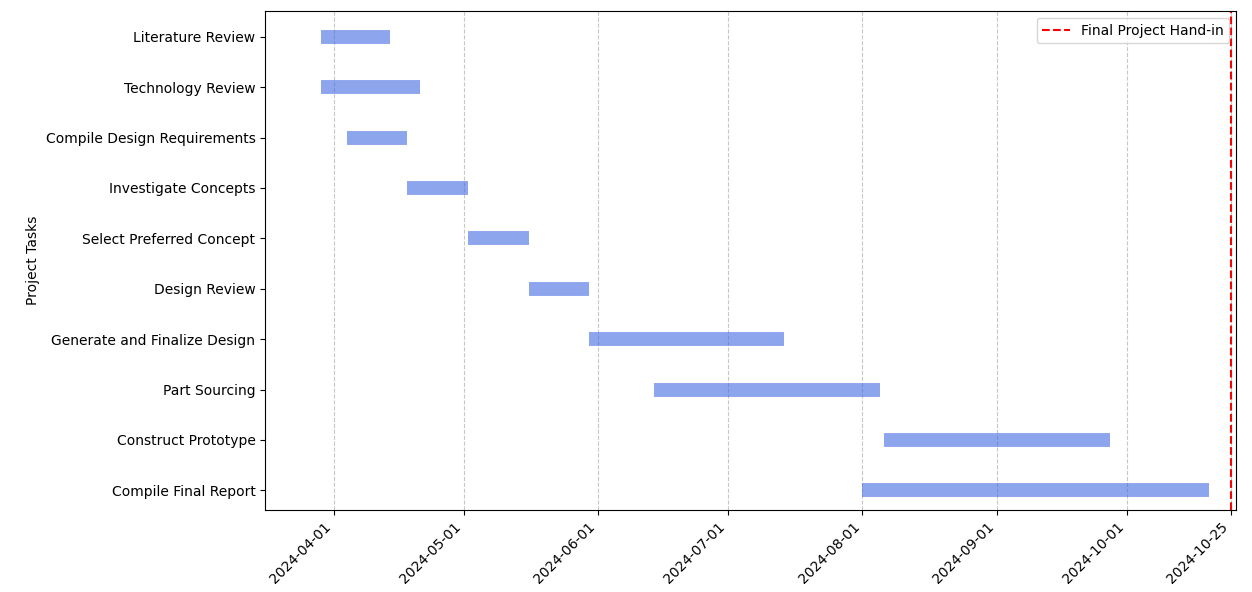
\includegraphics[width=1\linewidth]{figs/gantt_final.png}
    \caption{Gantt chart showing project timeline}
    \label{fig:gantt_final}
\end{figure}

\chapter{Responsible Use of Resources and End-of-Life Strategy}

Responsible resource use was a key consideration from the outset of the design process. Designs and drawings were thoroughly checked for accuracy to minimize waste from iterations, redesigns, or remanufacturing. Appropriate calculations and simulations were conducted to reduce the need for redesign. Where possible, low-impact materials were selected. For instance, standard, readily available, and low-cost steel tubing and shafts were used for the frame, while wood was chosen for the panels, which can be reused if needed, rather than opting for specialized materials.

In an effort to avoid waste, the system will be commissioned for long-term use, as it will be sold to a private buyer for personal use, ensuring its continued functionality. If the system is decommissioned in the future, most of the steel components can be disassembled and returned to the workshop for reuse in future projects, as very few parts were machined in a way that would prevent them from being repurposed. The wooden components can also be reused, and any parts that cannot be reused will be recycled where possible.

\include{chaps-append/chap-Planning-Details}
\include{chaps-append/chap-Self-ECSA}
\include{chaps-append/chap-End-of-Life}
\chapter{Safety Reports}

\section{Structures Lab Safety Report}

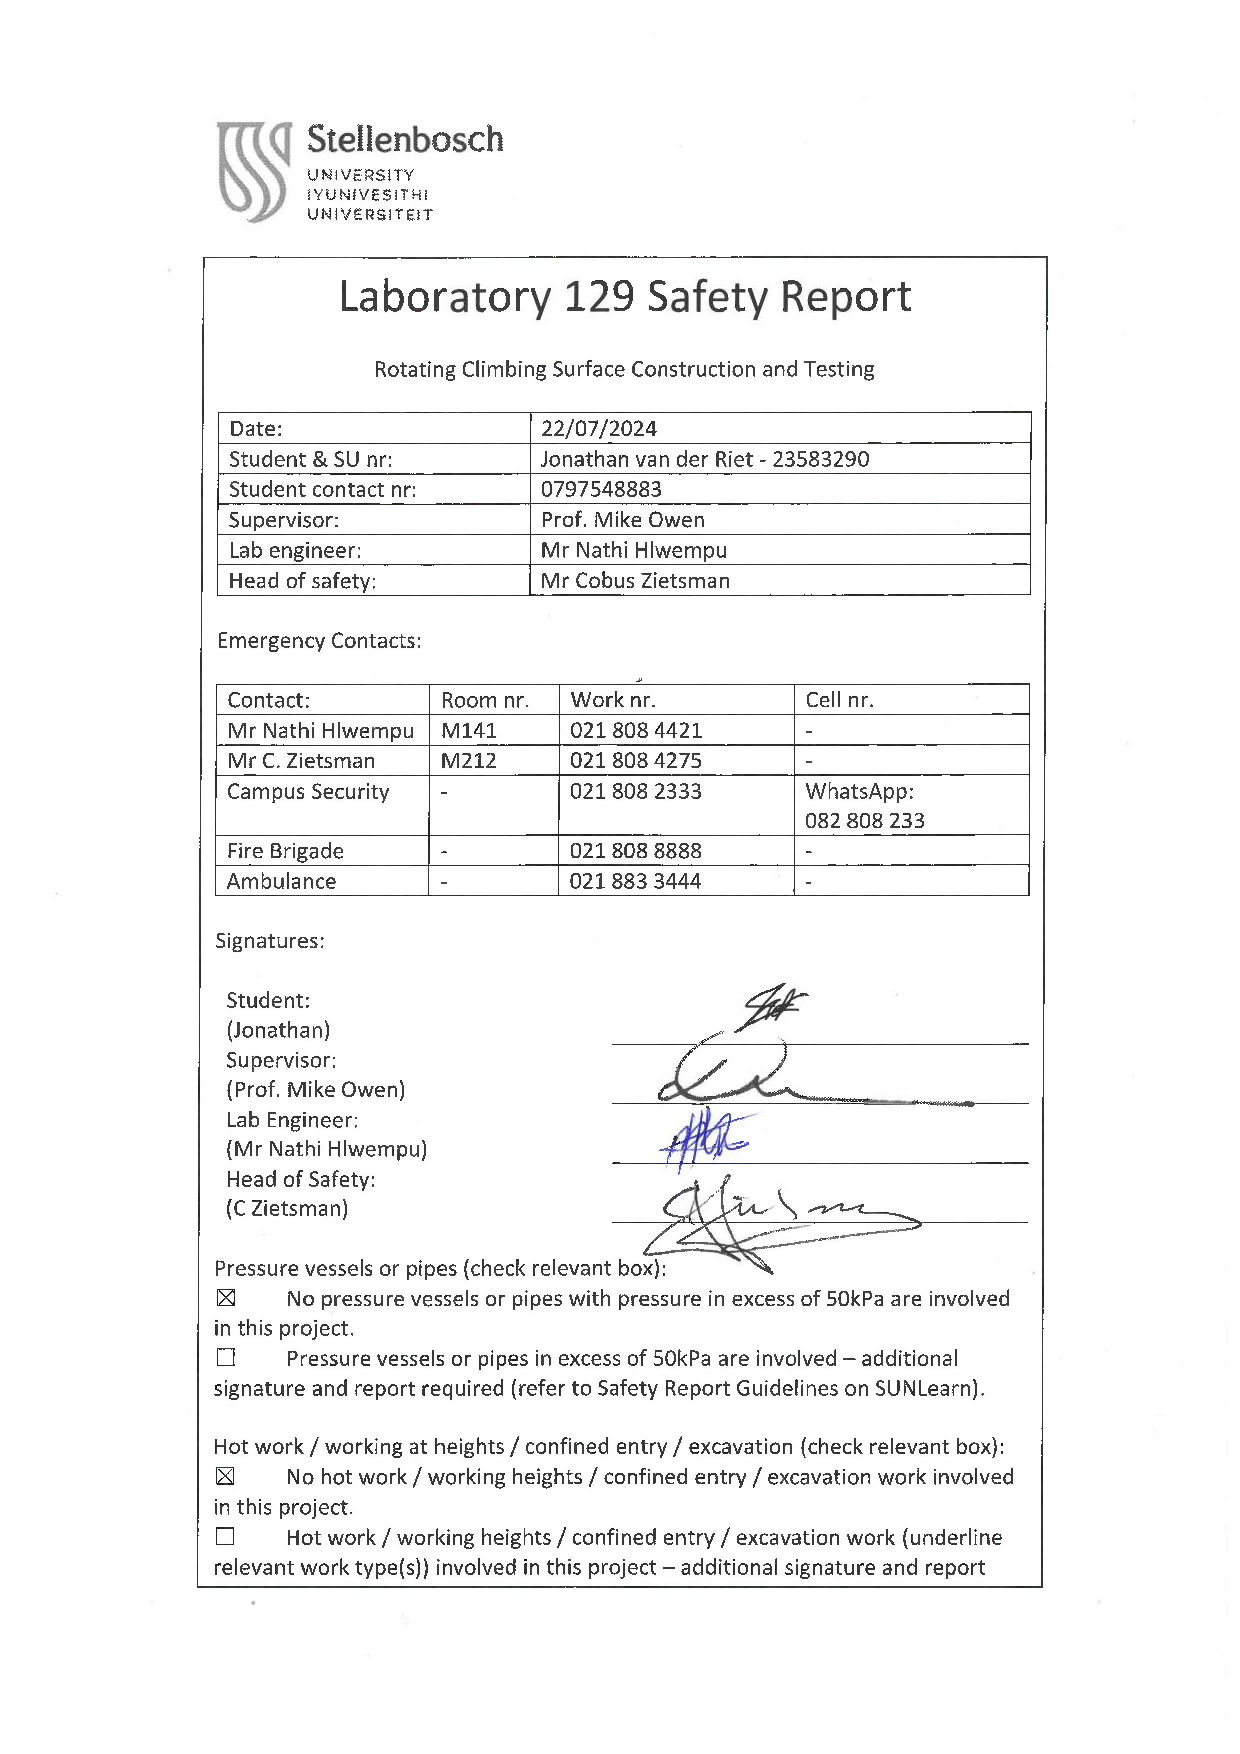
\includepdf[pages=-,scale=0.9]{chaps-append/23583290_Structures_Safety_Report.pdf}

\section{Mechatronics Lab Safety Report}

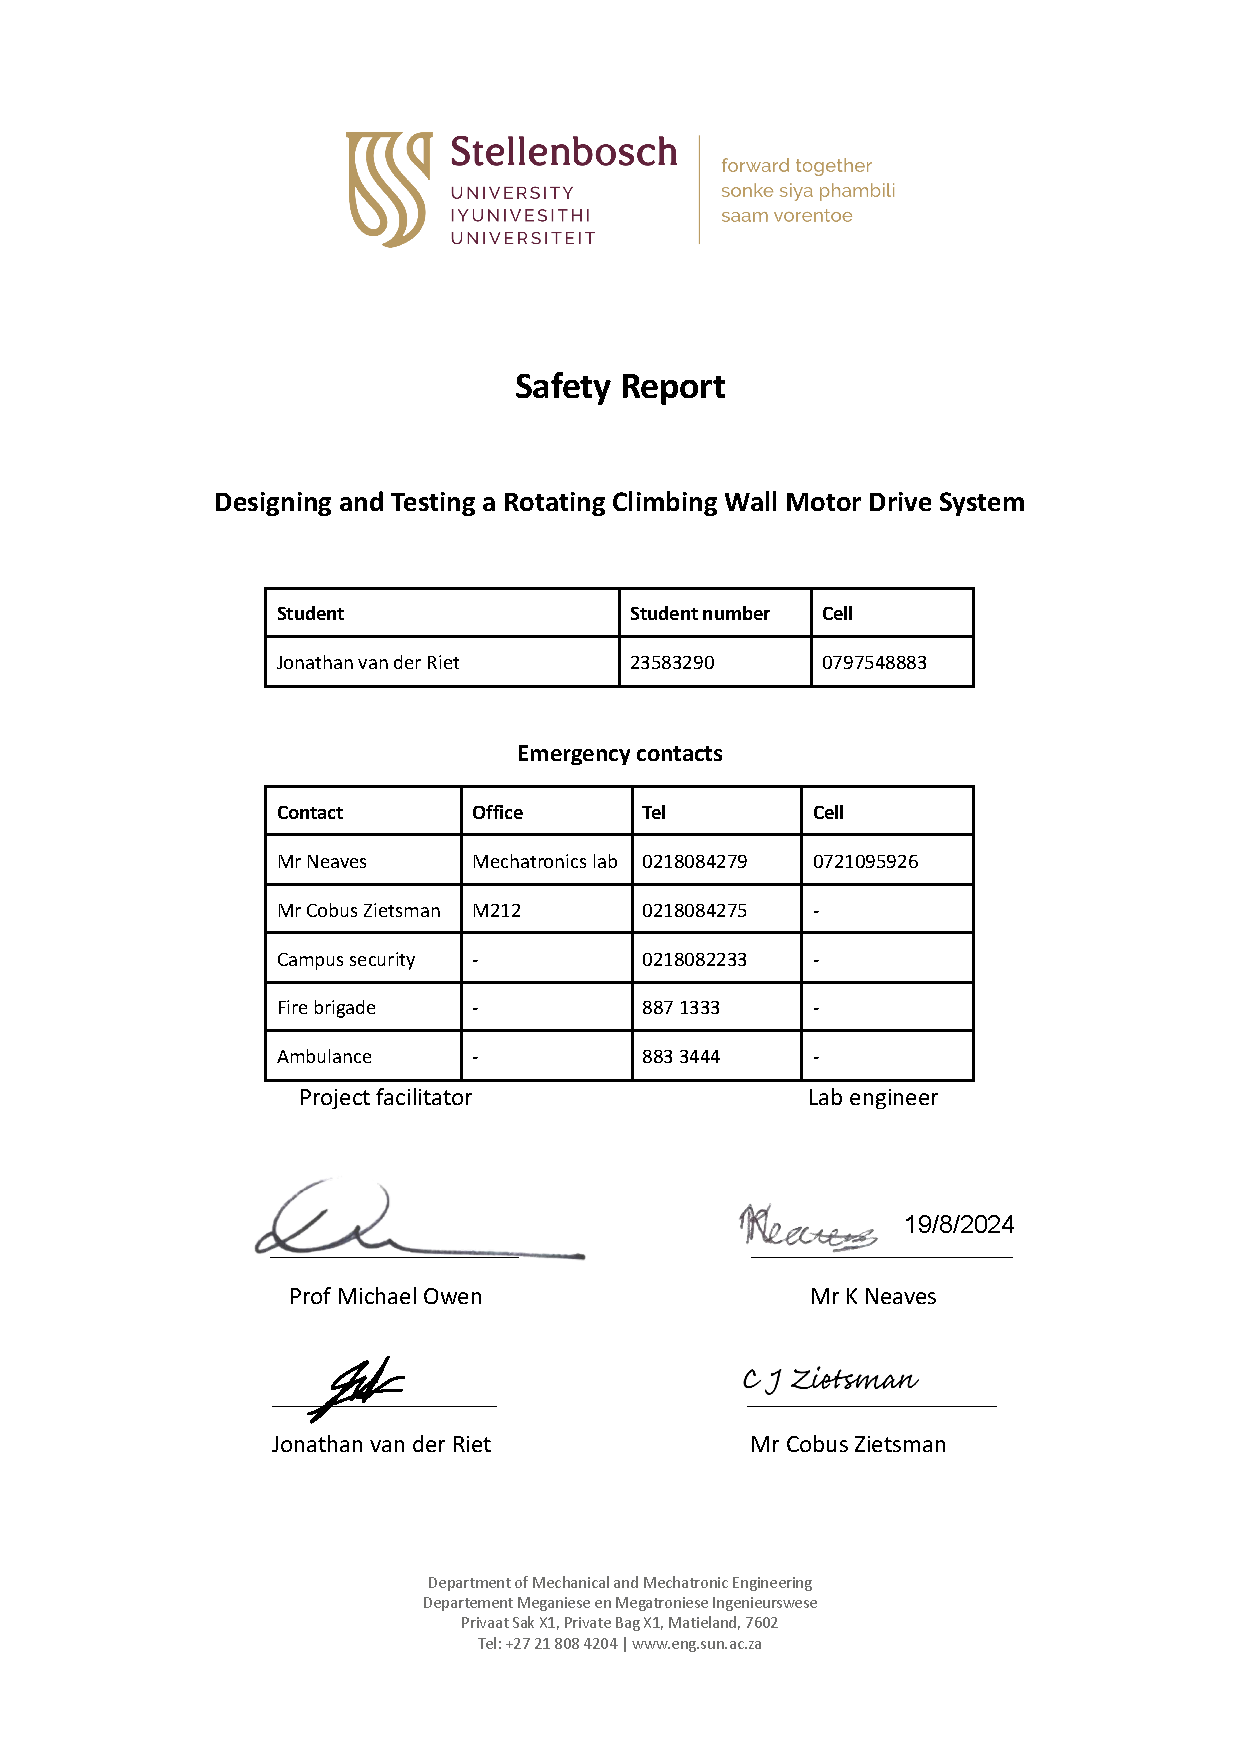
\includepdf[pages=-,scale=0.9]{chaps-append/Mech_Labs_Safety_Report_MO-2.pdf}




% Now include the back matter (bibliography, index, etc.)
\backmatter%----------------------------------------------------------
\bibliography{bib/bib-sample}

\end{document}
